% generated from JIRA project LVV
% using template at /opt/hostedtoolcache/Python/3.11.14/x64/lib/python3.11/site-packages/docsteady/templates/tpr.latex.jinja2.
% using docsteady version 3.1.0
% Please do not edit -- update information in Jira instead
\documentclass[DM,lsstdraft,STR,toc]{lsstdoc}
\usepackage{geometry}
\usepackage{longtable,booktabs}
\usepackage{enumitem}
\usepackage{arydshln}
\usepackage{attachfile}
\usepackage{array}
\usepackage{dashrule}
\usepackage{pdfpages}

\newcolumntype{L}[1]{>{\raggedright\let\newline\\\arraybackslash\hspace{0pt}}p{#1}}

\input{meta.tex}

\newcommand{\attachmentsUrl}{https://github.com/\gitorg/\lsstDocType-\lsstDocNum/blob/\gitref/attachments}
\providecommand{\tightlist}{
  \setlength{\itemsep}{0pt}\setlength{\parskip}{0pt}}

\setcounter{tocdepth}{4}

\providecommand{\ul}[1]{\textbf{#1}}


% Pandoc >= 3.2.1 introduces \pandocbounded; fallback for older/custom templates
\providecommand{\pandocbounded}[1]{#1}

\begin{document}

\def\milestoneName{LDM-503-19 (All P1a and 1b DM requirements verified)}
\def\milestoneId{}
\def\product{Acceptance}

\setDocCompact{true}

\title{LVV-P128: LDM-503-19 (All P1a and 1b DM requirements verified) Test Plan and Report}
\setDocRef{\lsstDocType-\lsstDocNum}
\date{ 2025-10-20 }
\author{ Jeffrey Carlin }

% Most recent last
\setDocChangeRecord{
\addtohist{}{2024-11-08}{First draft}{Jeffrey Carlin}
}

\setDocCurator{Jeffrey Carlin}
\setDocUpstreamLocation{\url{https://github.com/lsst-dm/\lsstDocType-\lsstDocNum}}
\setDocUpstreamVersion{\vcsRevision}



\setDocAbstract{
This is the test plan and report for
\textbf{ LDM-503-19 (All P1a and 1b DM requirements verified)},
an LSST milestone pertaining to the Data Management Subsystem.\\
This document is based on content automatically extracted from the Jira test database on \docDate.
The most recent change to the document repository was on \vcsDate.
}


\maketitle

\section{Introduction}
\label{sect:intro}


\subsection{Objectives}
\label{sect:objectives}

 This DM acceptance test campaign will verify all DM priority 1a and 1b
requirements that have not been verified as part of prior testing and
milestones.



\subsection{System Overview}
\label{sect:systemoverview}

 This test campaign is intended to verify that the DM system satisfies
all of the priority 1a and 1b requirements outlined in the Data
Management System Requirements (DMSR;~
\protect\phantomsection\label{isPasted}\href{https://lse-61.lsst.io/}{LSE-61}
), ensuring that we are progressing toward readiness for LSSTCam on-sky
observing. Additional DMSR requirements (priorities 2 and 3) will be
verified in later Acceptance Test Campaigns.\\
\strut \\
\textbf{Applicable Documents:}\\
\citeds{LSE-61}: Data Management System (DMS) Requirements\\
\citeds{LDM-503} Data Management Test Plan\\
\citeds{LDM-639}: Data Management Acceptance Test Specification\\
\strut \\
Tests in this campaign will use data products and artifacts from Data
Preview 0.2, which consists of DESC Data Challenge 2 (DC2) simulated
data reprocessed using the LSST Science Pipelines, on-sky data from
auxTel and LSSTComCam imaging campaigns, precursor data from
Subaru+HyperSuprime-Cam (HSC), and camera test-stand data, when
appropriate.


\subsection{Document Overview}
\label{sect:docoverview}

This document was generated from Jira, obtaining the relevant information from the
\href{https://rubinobs.atlassian.net/projects/LVV?selectedItem=com.atlassian.plugins.atlassian-connect-plugin:com.kanoah.test-manager__main-project-page\#\!/v2/testPlan/LVV-P128}{LVV-P128}
~Jira Test Plan and related Test Cycles (
\href{https://rubinobs.atlassian.net/projects/LVV?selectedItem=com.atlassian.plugins.atlassian-connect-plugin:com.kanoah.test-manager__main-project-page\#\!/testPlayer/LVV-R293}{LVV-R293}
).

Section \ref{sect:intro} provides an overview of the test campaign, the system under test (\product{}),
the applicable documentation, and explains how this document is organized.
Section \ref{sect:testplan} provides additional information about the test plan, like for example the configuration
used for this test or related documentation.
Section \ref{sect:personnel} describes the necessary roles and lists the individuals assigned to them.

Section \ref{sect:overview} provides a summary of the test results, including an overview in Table \ref{table:summary},
an overall assessment statement and suggestions for possible improvements.
Section \ref{sect:detailedtestresults} provides detailed results for each step in each test case.

The current status of test plan \href{https://rubinobs.atlassian.net/projects/LVV?selectedItem=com.atlassian.plugins.atlassian-connect-plugin:com.kanoah.test-manager__main-project-page\#\!/v2/testPlan/LVV-P128}{LVV-P128} in Jira is \textbf{ Approved }.

\subsection{References}
\label{sect:references}
\renewcommand{\refname}{}
\bibliography{lsst,refs,books,refs_ads,local}


\newpage
\section{Test Plan Details}
\label{sect:testplan}


\subsection{Data Collection}

  Observing is not required for this test campaign.

\subsection{Verification Environment}
\label{sect:hwconf}
  Most testing will be performed using the Rubin Science Platform (RSP)
and the development cluster at the USDF. All tests will use the most
recent available version of the Pipelines.

  \subsection{Entry Criteria}
  None

  \subsection{Exit Criteria}
  None


\subsection{Related Documentation}

Docushare collection where additional relevant documentation can be found:

\begin{itemize}
\item None
\end{itemize}


\subsection{PMCS Activity}

Primavera milestones related to the test campaign:
None


\newpage
\section{Personnel}
\label{sect:personnel}

The personnel involved in the test campaign is shown in the following table.

{\small
\begin{longtable}{p{3cm}p{3cm}p{3cm}p{6cm}}
\hline
\multicolumn{2}{r}{T. Plan \href{https://rubinobs.atlassian.net/projects/LVV?selectedItem=com.atlassian.plugins.atlassian-connect-plugin:com.kanoah.test-manager__main-project-page\#\!/v2/testPlan/LVV-P128}{LVV-P128} owner:} &
\multicolumn{2}{l}{\textbf{ Jeffrey Carlin } }\\\hline
\multicolumn{2}{r}{T. Cycle \href{https://rubinobs.atlassian.net/projects/LVV?selectedItem=com.atlassian.plugins.atlassian-connect-plugin:com.kanoah.test-manager__main-project-page\#\!/testPlayer/LVV-R293}{LVV-R293} owner:} &
\multicolumn{2}{l}{\textbf{
Jeffrey Carlin }
} \\\hline
\textbf{Test Cases} & \textbf{Assigned to} & \textbf{Executed by} & \textbf{Additional Test Personnel} \\ \hline

\href{https://rubinobs.atlassian.net/projects/LVV?selectedItem=com.atlassian.plugins.atlassian-connect-plugin:com.kanoah.test-manager__main-project-page\#\!/v2/testCase/LVV-T2328}{LVV-T2328}
& {\small Leanne Guy } & {\small Undefined } &
\begin{minipage}[]{6cm}
\smallskip
{\small  }
\medskip
\end{minipage}
\\ \hline

\href{https://rubinobs.atlassian.net/projects/LVV?selectedItem=com.atlassian.plugins.atlassian-connect-plugin:com.kanoah.test-manager__main-project-page\#\!/v2/testCase/LVV-T2329}{LVV-T2329}
& {\small Leanne Guy } & {\small Undefined } &
\begin{minipage}[]{6cm}
\smallskip
{\small  }
\medskip
\end{minipage}
\\ \hline

\href{https://rubinobs.atlassian.net/projects/LVV?selectedItem=com.atlassian.plugins.atlassian-connect-plugin:com.kanoah.test-manager__main-project-page\#\!/v2/testCase/LVV-T1563}{LVV-T1563}
& {\small Jeffrey Carlin } & {\small Undefined } &
\begin{minipage}[]{6cm}
\smallskip
{\small  }
\medskip
\end{minipage}
\\ \hline

\href{https://rubinobs.atlassian.net/projects/LVV?selectedItem=com.atlassian.plugins.atlassian-connect-plugin:com.kanoah.test-manager__main-project-page\#\!/v2/testCase/LVV-T1564}{LVV-T1564}
& {\small Jeffrey Carlin } & {\small Undefined } &
\begin{minipage}[]{6cm}
\smallskip
{\small  }
\medskip
\end{minipage}
\\ \hline

\href{https://rubinobs.atlassian.net/projects/LVV?selectedItem=com.atlassian.plugins.atlassian-connect-plugin:com.kanoah.test-manager__main-project-page\#\!/v2/testCase/LVV-T1562}{LVV-T1562}
& {\small Jeffrey Carlin } & {\small Undefined } &
\begin{minipage}[]{6cm}
\smallskip
{\small  }
\medskip
\end{minipage}
\\ \hline

\href{https://rubinobs.atlassian.net/projects/LVV?selectedItem=com.atlassian.plugins.atlassian-connect-plugin:com.kanoah.test-manager__main-project-page\#\!/v2/testCase/LVV-T1561}{LVV-T1561}
& {\small Jeffrey Carlin } & {\small Undefined } &
\begin{minipage}[]{6cm}
\smallskip
{\small  }
\medskip
\end{minipage}
\\ \hline

\href{https://rubinobs.atlassian.net/projects/LVV?selectedItem=com.atlassian.plugins.atlassian-connect-plugin:com.kanoah.test-manager__main-project-page\#\!/v2/testCase/LVV-T1560}{LVV-T1560}
& {\small Jeffrey Carlin } & {\small Undefined } &
\begin{minipage}[]{6cm}
\smallskip
{\small  }
\medskip
\end{minipage}
\\ \hline

\href{https://rubinobs.atlassian.net/projects/LVV?selectedItem=com.atlassian.plugins.atlassian-connect-plugin:com.kanoah.test-manager__main-project-page\#\!/v2/testCase/LVV-T1528}{LVV-T1528}
& {\small Jeffrey Carlin } & {\small Undefined } &
\begin{minipage}[]{6cm}
\smallskip
{\small  }
\medskip
\end{minipage}
\\ \hline

\href{https://rubinobs.atlassian.net/projects/LVV?selectedItem=com.atlassian.plugins.atlassian-connect-plugin:com.kanoah.test-manager__main-project-page\#\!/v2/testCase/LVV-T1524}{LVV-T1524}
& {\small Jeffrey Carlin } & {\small Undefined } &
\begin{minipage}[]{6cm}
\smallskip
{\small  }
\medskip
\end{minipage}
\\ \hline

\href{https://rubinobs.atlassian.net/projects/LVV?selectedItem=com.atlassian.plugins.atlassian-connect-plugin:com.kanoah.test-manager__main-project-page\#\!/v2/testCase/LVV-T1530}{LVV-T1530}
& {\small Jeffrey Carlin } & {\small Undefined } &
\begin{minipage}[]{6cm}
\smallskip
{\small  }
\medskip
\end{minipage}
\\ \hline

\href{https://rubinobs.atlassian.net/projects/LVV?selectedItem=com.atlassian.plugins.atlassian-connect-plugin:com.kanoah.test-manager__main-project-page\#\!/v2/testCase/LVV-T2905}{LVV-T2905}
& {\small Leanne Guy } & {\small Undefined } &
\begin{minipage}[]{6cm}
\smallskip
{\small  }
\medskip
\end{minipage}
\\ \hline

\href{https://rubinobs.atlassian.net/projects/LVV?selectedItem=com.atlassian.plugins.atlassian-connect-plugin:com.kanoah.test-manager__main-project-page\#\!/v2/testCase/LVV-T1332}{LVV-T1332}
& {\small Leanne Guy } & {\small Undefined } &
\begin{minipage}[]{6cm}
\smallskip
{\small  }
\medskip
\end{minipage}
\\ \hline

\href{https://rubinobs.atlassian.net/projects/LVV?selectedItem=com.atlassian.plugins.atlassian-connect-plugin:com.kanoah.test-manager__main-project-page\#\!/v2/testCase/LVV-T385}{LVV-T385}
& {\small Leanne Guy } & {\small Undefined } &
\begin{minipage}[]{6cm}
\smallskip
{\small  }
\medskip
\end{minipage}
\\ \hline

\href{https://rubinobs.atlassian.net/projects/LVV?selectedItem=com.atlassian.plugins.atlassian-connect-plugin:com.kanoah.test-manager__main-project-page\#\!/v2/testCase/LVV-T2901}{LVV-T2901}
& {\small Leanne Guy } & {\small Undefined } &
\begin{minipage}[]{6cm}
\smallskip
{\small  }
\medskip
\end{minipage}
\\ \hline

\href{https://rubinobs.atlassian.net/projects/LVV?selectedItem=com.atlassian.plugins.atlassian-connect-plugin:com.kanoah.test-manager__main-project-page\#\!/v2/testCase/LVV-T2900}{LVV-T2900}
& {\small Leanne Guy } & {\small Undefined } &
\begin{minipage}[]{6cm}
\smallskip
{\small  }
\medskip
\end{minipage}
\\ \hline

\href{https://rubinobs.atlassian.net/projects/LVV?selectedItem=com.atlassian.plugins.atlassian-connect-plugin:com.kanoah.test-manager__main-project-page\#\!/v2/testCase/LVV-T168}{LVV-T168}
& {\small Jeffrey Carlin } & {\small Undefined } &
\begin{minipage}[]{6cm}
\smallskip
{\small  }
\medskip
\end{minipage}
\\ \hline

\href{https://rubinobs.atlassian.net/projects/LVV?selectedItem=com.atlassian.plugins.atlassian-connect-plugin:com.kanoah.test-manager__main-project-page\#\!/v2/testCase/LVV-T2177}{LVV-T2177}
& {\small Jeffrey Carlin } & {\small Undefined } &
\begin{minipage}[]{6cm}
\smallskip
{\small  }
\medskip
\end{minipage}
\\ \hline

\href{https://rubinobs.atlassian.net/projects/LVV?selectedItem=com.atlassian.plugins.atlassian-connect-plugin:com.kanoah.test-manager__main-project-page\#\!/v2/testCase/LVV-T1755}{LVV-T1755}
& {\small Jeffrey Carlin } & {\small Undefined } &
\begin{minipage}[]{6cm}
\smallskip
{\small  }
\medskip
\end{minipage}
\\ \hline

\href{https://rubinobs.atlassian.net/projects/LVV?selectedItem=com.atlassian.plugins.atlassian-connect-plugin:com.kanoah.test-manager__main-project-page\#\!/v2/testCase/LVV-T2176}{LVV-T2176}
& {\small Jeffrey Carlin } & {\small Undefined } &
\begin{minipage}[]{6cm}
\smallskip
{\small  }
\medskip
\end{minipage}
\\ \hline

\href{https://rubinobs.atlassian.net/projects/LVV?selectedItem=com.atlassian.plugins.atlassian-connect-plugin:com.kanoah.test-manager__main-project-page\#\!/v2/testCase/LVV-T1754}{LVV-T1754}
& {\small Jeffrey Carlin } & {\small Undefined } &
\begin{minipage}[]{6cm}
\smallskip
{\small  }
\medskip
\end{minipage}
\\ \hline

\href{https://rubinobs.atlassian.net/projects/LVV?selectedItem=com.atlassian.plugins.atlassian-connect-plugin:com.kanoah.test-manager__main-project-page\#\!/v2/testCase/LVV-T376}{LVV-T376}
& {\small Leanne Guy } & {\small Undefined } &
\begin{minipage}[]{6cm}
\smallskip
{\small  }
\medskip
\end{minipage}
\\ \hline

\href{https://rubinobs.atlassian.net/projects/LVV?selectedItem=com.atlassian.plugins.atlassian-connect-plugin:com.kanoah.test-manager__main-project-page\#\!/v2/testCase/LVV-T2724}{LVV-T2724}
& {\small Leanne Guy } & {\small Undefined } &
\begin{minipage}[]{6cm}
\smallskip
{\small  }
\medskip
\end{minipage}
\\ \hline

\href{https://rubinobs.atlassian.net/projects/LVV?selectedItem=com.atlassian.plugins.atlassian-connect-plugin:com.kanoah.test-manager__main-project-page\#\!/v2/testCase/LVV-T2899}{LVV-T2899}
& {\small Leanne Guy } & {\small Undefined } &
\begin{minipage}[]{6cm}
\smallskip
{\small  }
\medskip
\end{minipage}
\\ \hline

\href{https://rubinobs.atlassian.net/projects/LVV?selectedItem=com.atlassian.plugins.atlassian-connect-plugin:com.kanoah.test-manager__main-project-page\#\!/v2/testCase/LVV-T2333}{LVV-T2333}
& {\small Leanne Guy } & {\small Undefined } &
\begin{minipage}[]{6cm}
\smallskip
{\small  }
\medskip
\end{minipage}
\\ \hline

\href{https://rubinobs.atlassian.net/projects/LVV?selectedItem=com.atlassian.plugins.atlassian-connect-plugin:com.kanoah.test-manager__main-project-page\#\!/v2/testCase/LVV-T2332}{LVV-T2332}
& {\small Leanne Guy } & {\small Undefined } &
\begin{minipage}[]{6cm}
\smallskip
{\small  }
\medskip
\end{minipage}
\\ \hline

\href{https://rubinobs.atlassian.net/projects/LVV?selectedItem=com.atlassian.plugins.atlassian-connect-plugin:com.kanoah.test-manager__main-project-page\#\!/v2/testCase/LVV-T2700}{LVV-T2700}
& {\small Leanne Guy } & {\small Undefined } &
\begin{minipage}[]{6cm}
\smallskip
{\small  }
\medskip
\end{minipage}
\\ \hline

\href{https://rubinobs.atlassian.net/projects/LVV?selectedItem=com.atlassian.plugins.atlassian-connect-plugin:com.kanoah.test-manager__main-project-page\#\!/v2/testCase/LVV-T27}{LVV-T27}
& {\small Jeffrey Carlin } & {\small Undefined } &
\begin{minipage}[]{6cm}
\smallskip
{\small  }
\medskip
\end{minipage}
\\ \hline

\href{https://rubinobs.atlassian.net/projects/LVV?selectedItem=com.atlassian.plugins.atlassian-connect-plugin:com.kanoah.test-manager__main-project-page\#\!/v2/testCase/LVV-T2331}{LVV-T2331}
& {\small Leanne Guy } & {\small Undefined } &
\begin{minipage}[]{6cm}
\smallskip
{\small  }
\medskip
\end{minipage}
\\ \hline

\href{https://rubinobs.atlassian.net/projects/LVV?selectedItem=com.atlassian.plugins.atlassian-connect-plugin:com.kanoah.test-manager__main-project-page\#\!/v2/testCase/LVV-T160}{LVV-T160}
& {\small Gregory Dubois-Felsmann } & {\small Undefined } &
\begin{minipage}[]{6cm}
\smallskip
{\small  }
\medskip
\end{minipage}
\\ \hline

\href{https://rubinobs.atlassian.net/projects/LVV?selectedItem=com.atlassian.plugins.atlassian-connect-plugin:com.kanoah.test-manager__main-project-page\#\!/v2/testCase/LVV-T159}{LVV-T159}
& {\small Simon Krughoff } & {\small Undefined } &
\begin{minipage}[]{6cm}
\smallskip
{\small  }
\medskip
\end{minipage}
\\ \hline

\href{https://rubinobs.atlassian.net/projects/LVV?selectedItem=com.atlassian.plugins.atlassian-connect-plugin:com.kanoah.test-manager__main-project-page\#\!/v2/testCase/LVV-T26}{LVV-T26}
& {\small Jeffrey Carlin } & {\small Jeffrey Carlin } &
\begin{minipage}[]{6cm}
\smallskip
{\small  }
\medskip
\end{minipage}
\\ \hline

\href{https://rubinobs.atlassian.net/projects/LVV?selectedItem=com.atlassian.plugins.atlassian-connect-plugin:com.kanoah.test-manager__main-project-page\#\!/v2/testCase/LVV-T24}{LVV-T24}
& {\small Jeffrey Carlin } & {\small Jeffrey Carlin } &
\begin{minipage}[]{6cm}
\smallskip
{\small  }
\medskip
\end{minipage}
\\ \hline

\href{https://rubinobs.atlassian.net/projects/LVV?selectedItem=com.atlassian.plugins.atlassian-connect-plugin:com.kanoah.test-manager__main-project-page\#\!/v2/testCase/LVV-T44}{LVV-T44}
& {\small Jeffrey Carlin } & {\small Undefined } &
\begin{minipage}[]{6cm}
\smallskip
{\small  }
\medskip
\end{minipage}
\\ \hline

\href{https://rubinobs.atlassian.net/projects/LVV?selectedItem=com.atlassian.plugins.atlassian-connect-plugin:com.kanoah.test-manager__main-project-page\#\!/v2/testCase/LVV-T58}{LVV-T58}
& {\small Eric Bellm } & {\small Undefined } &
\begin{minipage}[]{6cm}
\smallskip
{\small  }
\medskip
\end{minipage}
\\ \hline

\href{https://rubinobs.atlassian.net/projects/LVV?selectedItem=com.atlassian.plugins.atlassian-connect-plugin:com.kanoah.test-manager__main-project-page\#\!/v2/testCase/LVV-T94}{LVV-T94}
& {\small Melissa Graham } & {\small Undefined } &
\begin{minipage}[]{6cm}
\smallskip
{\small  }
\medskip
\end{minipage}
\\ \hline

\href{https://rubinobs.atlassian.net/projects/LVV?selectedItem=com.atlassian.plugins.atlassian-connect-plugin:com.kanoah.test-manager__main-project-page\#\!/v2/testCase/LVV-T56}{LVV-T56}
& {\small Eric Bellm } & {\small Undefined } &
\begin{minipage}[]{6cm}
\smallskip
{\small  }
\medskip
\end{minipage}
\\ \hline

\href{https://rubinobs.atlassian.net/projects/LVV?selectedItem=com.atlassian.plugins.atlassian-connect-plugin:com.kanoah.test-manager__main-project-page\#\!/v2/testCase/LVV-T180}{LVV-T180}
& {\small Leanne Guy } & {\small Undefined } &
\begin{minipage}[]{6cm}
\smallskip
{\small  }
\medskip
\end{minipage}
\\ \hline

\href{https://rubinobs.atlassian.net/projects/LVV?selectedItem=com.atlassian.plugins.atlassian-connect-plugin:com.kanoah.test-manager__main-project-page\#\!/v2/testCase/LVV-T179}{LVV-T179}
& {\small Leanne Guy } & {\small Undefined } &
\begin{minipage}[]{6cm}
\smallskip
{\small  }
\medskip
\end{minipage}
\\ \hline

\href{https://rubinobs.atlassian.net/projects/LVV?selectedItem=com.atlassian.plugins.atlassian-connect-plugin:com.kanoah.test-manager__main-project-page\#\!/v2/testCase/LVV-T158}{LVV-T158}
& {\small Jeffrey Carlin } & {\small Undefined } &
\begin{minipage}[]{6cm}
\smallskip
{\small  }
\medskip
\end{minipage}
\\ \hline

\href{https://rubinobs.atlassian.net/projects/LVV?selectedItem=com.atlassian.plugins.atlassian-connect-plugin:com.kanoah.test-manager__main-project-page\#\!/v2/testCase/LVV-T157}{LVV-T157}
& {\small Jeffrey Carlin } & {\small Undefined } &
\begin{minipage}[]{6cm}
\smallskip
{\small  }
\medskip
\end{minipage}
\\ \hline

\href{https://rubinobs.atlassian.net/projects/LVV?selectedItem=com.atlassian.plugins.atlassian-connect-plugin:com.kanoah.test-manager__main-project-page\#\!/v2/testCase/LVV-T156}{LVV-T156}
& {\small Leanne Guy } & {\small Undefined } &
\begin{minipage}[]{6cm}
\smallskip
{\small  }
\medskip
\end{minipage}
\\ \hline

\href{https://rubinobs.atlassian.net/projects/LVV?selectedItem=com.atlassian.plugins.atlassian-connect-plugin:com.kanoah.test-manager__main-project-page\#\!/v2/testCase/LVV-T155}{LVV-T155}
& {\small Robert Gruendl } & {\small Undefined } &
\begin{minipage}[]{6cm}
\smallskip
{\small  }
\medskip
\end{minipage}
\\ \hline

\href{https://rubinobs.atlassian.net/projects/LVV?selectedItem=com.atlassian.plugins.atlassian-connect-plugin:com.kanoah.test-manager__main-project-page\#\!/v2/testCase/LVV-T124}{LVV-T124}
& {\small Jeffrey Carlin } & {\small Undefined } &
\begin{minipage}[]{6cm}
\smallskip
{\small  }
\medskip
\end{minipage}
\\ \hline

\href{https://rubinobs.atlassian.net/projects/LVV?selectedItem=com.atlassian.plugins.atlassian-connect-plugin:com.kanoah.test-manager__main-project-page\#\!/v2/testCase/LVV-T147}{LVV-T147}
& {\small Robert Gruendl } & {\small Undefined } &
\begin{minipage}[]{6cm}
\smallskip
{\small  }
\medskip
\end{minipage}
\\ \hline

\href{https://rubinobs.atlassian.net/projects/LVV?selectedItem=com.atlassian.plugins.atlassian-connect-plugin:com.kanoah.test-manager__main-project-page\#\!/v2/testCase/LVV-T138}{LVV-T138}
& {\small Leanne Guy } & {\small Leanne Guy } &
\begin{minipage}[]{6cm}
\smallskip
{\small  }
\medskip
\end{minipage}
\\ \hline

\href{https://rubinobs.atlassian.net/projects/LVV?selectedItem=com.atlassian.plugins.atlassian-connect-plugin:com.kanoah.test-manager__main-project-page\#\!/v2/testCase/LVV-T99}{LVV-T99}
& {\small Jeffrey Carlin } & {\small Undefined } &
\begin{minipage}[]{6cm}
\smallskip
{\small  }
\medskip
\end{minipage}
\\ \hline

\href{https://rubinobs.atlassian.net/projects/LVV?selectedItem=com.atlassian.plugins.atlassian-connect-plugin:com.kanoah.test-manager__main-project-page\#\!/v2/testCase/LVV-T96}{LVV-T96}
& {\small Jeffrey Carlin } & {\small Undefined } &
\begin{minipage}[]{6cm}
\smallskip
{\small  }
\medskip
\end{minipage}
\\ \hline

\href{https://rubinobs.atlassian.net/projects/LVV?selectedItem=com.atlassian.plugins.atlassian-connect-plugin:com.kanoah.test-manager__main-project-page\#\!/v2/testCase/LVV-T110}{LVV-T110}
& {\small Eric Bellm } & {\small Undefined } &
\begin{minipage}[]{6cm}
\smallskip
{\small  }
\medskip
\end{minipage}
\\ \hline

\href{https://rubinobs.atlassian.net/projects/LVV?selectedItem=com.atlassian.plugins.atlassian-connect-plugin:com.kanoah.test-manager__main-project-page\#\!/v2/testCase/LVV-T108}{LVV-T108}
& {\small Jeffrey Carlin } & {\small Undefined } &
\begin{minipage}[]{6cm}
\smallskip
{\small  }
\medskip
\end{minipage}
\\ \hline

\href{https://rubinobs.atlassian.net/projects/LVV?selectedItem=com.atlassian.plugins.atlassian-connect-plugin:com.kanoah.test-manager__main-project-page\#\!/v2/testCase/LVV-T107}{LVV-T107}
& {\small Eric Bellm } & {\small Undefined } &
\begin{minipage}[]{6cm}
\smallskip
{\small  }
\medskip
\end{minipage}
\\ \hline

\href{https://rubinobs.atlassian.net/projects/LVV?selectedItem=com.atlassian.plugins.atlassian-connect-plugin:com.kanoah.test-manager__main-project-page\#\!/v2/testCase/LVV-T91}{LVV-T91}
& {\small Jeffrey Carlin } & {\small Undefined } &
\begin{minipage}[]{6cm}
\smallskip
{\small  }
\medskip
\end{minipage}
\\ \hline

\href{https://rubinobs.atlassian.net/projects/LVV?selectedItem=com.atlassian.plugins.atlassian-connect-plugin:com.kanoah.test-manager__main-project-page\#\!/v2/testCase/LVV-T75}{LVV-T75}
& {\small Jeffrey Carlin } & {\small Undefined } &
\begin{minipage}[]{6cm}
\smallskip
{\small  }
\medskip
\end{minipage}
\\ \hline

\href{https://rubinobs.atlassian.net/projects/LVV?selectedItem=com.atlassian.plugins.atlassian-connect-plugin:com.kanoah.test-manager__main-project-page\#\!/v2/testCase/LVV-T74}{LVV-T74}
& {\small Jeffrey Carlin } & {\small Jeffrey Carlin } &
\begin{minipage}[]{6cm}
\smallskip
{\small  }
\medskip
\end{minipage}
\\ \hline

\href{https://rubinobs.atlassian.net/projects/LVV?selectedItem=com.atlassian.plugins.atlassian-connect-plugin:com.kanoah.test-manager__main-project-page\#\!/v2/testCase/LVV-T73}{LVV-T73}
& {\small Jeffrey Carlin } & {\small Jeffrey Carlin } &
\begin{minipage}[]{6cm}
\smallskip
{\small  }
\medskip
\end{minipage}
\\ \hline

\href{https://rubinobs.atlassian.net/projects/LVV?selectedItem=com.atlassian.plugins.atlassian-connect-plugin:com.kanoah.test-manager__main-project-page\#\!/v2/testCase/LVV-T69}{LVV-T69}
& {\small Jeffrey Carlin } & {\small Undefined } &
\begin{minipage}[]{6cm}
\smallskip
{\small  }
\medskip
\end{minipage}
\\ \hline

\href{https://rubinobs.atlassian.net/projects/LVV?selectedItem=com.atlassian.plugins.atlassian-connect-plugin:com.kanoah.test-manager__main-project-page\#\!/v2/testCase/LVV-T67}{LVV-T67}
& {\small Jeffrey Carlin } & {\small Undefined } &
\begin{minipage}[]{6cm}
\smallskip
{\small  }
\medskip
\end{minipage}
\\ \hline

\href{https://rubinobs.atlassian.net/projects/LVV?selectedItem=com.atlassian.plugins.atlassian-connect-plugin:com.kanoah.test-manager__main-project-page\#\!/v2/testCase/LVV-T54}{LVV-T54}
& {\small Eric Bellm } & {\small Undefined } &
\begin{minipage}[]{6cm}
\smallskip
{\small  }
\medskip
\end{minipage}
\\ \hline

\href{https://rubinobs.atlassian.net/projects/LVV?selectedItem=com.atlassian.plugins.atlassian-connect-plugin:com.kanoah.test-manager__main-project-page\#\!/v2/testCase/LVV-T52}{LVV-T52}
& {\small Eric Bellm } & {\small Undefined } &
\begin{minipage}[]{6cm}
\smallskip
{\small  }
\medskip
\end{minipage}
\\ \hline

\href{https://rubinobs.atlassian.net/projects/LVV?selectedItem=com.atlassian.plugins.atlassian-connect-plugin:com.kanoah.test-manager__main-project-page\#\!/v2/testCase/LVV-T2305}{LVV-T2305}
& {\small Leanne Guy } & {\small Undefined } &
\begin{minipage}[]{6cm}
\smallskip
{\small  }
\medskip
\end{minipage}
\\ \hline

\href{https://rubinobs.atlassian.net/projects/LVV?selectedItem=com.atlassian.plugins.atlassian-connect-plugin:com.kanoah.test-manager__main-project-page\#\!/v2/testCase/LVV-T2304}{LVV-T2304}
& {\small Leanne Guy } & {\small Undefined } &
\begin{minipage}[]{6cm}
\smallskip
{\small  }
\medskip
\end{minipage}
\\ \hline

\href{https://rubinobs.atlassian.net/projects/LVV?selectedItem=com.atlassian.plugins.atlassian-connect-plugin:com.kanoah.test-manager__main-project-page\#\!/v2/testCase/LVV-T51}{LVV-T51}
& {\small Eric Bellm } & {\small Undefined } &
\begin{minipage}[]{6cm}
\smallskip
{\small  }
\medskip
\end{minipage}
\\ \hline

\href{https://rubinobs.atlassian.net/projects/LVV?selectedItem=com.atlassian.plugins.atlassian-connect-plugin:com.kanoah.test-manager__main-project-page\#\!/v2/testCase/LVV-T49}{LVV-T49}
& {\small Eric Bellm } & {\small Undefined } &
\begin{minipage}[]{6cm}
\smallskip
{\small  }
\medskip
\end{minipage}
\\ \hline

\href{https://rubinobs.atlassian.net/projects/LVV?selectedItem=com.atlassian.plugins.atlassian-connect-plugin:com.kanoah.test-manager__main-project-page\#\!/v2/testCase/LVV-T65}{LVV-T65}
& {\small Jeffrey Carlin } & {\small Jeffrey Carlin } &
\begin{minipage}[]{6cm}
\smallskip
{\small  }
\medskip
\end{minipage}
\\ \hline

\href{https://rubinobs.atlassian.net/projects/LVV?selectedItem=com.atlassian.plugins.atlassian-connect-plugin:com.kanoah.test-manager__main-project-page\#\!/v2/testCase/LVV-T211}{LVV-T211}
& {\small Kian-Tat Lim } & {\small Kevin Siruno } &
\begin{minipage}[]{6cm}
\smallskip
{\small  }
\medskip
\end{minipage}
\\ \hline

\href{https://rubinobs.atlassian.net/projects/LVV?selectedItem=com.atlassian.plugins.atlassian-connect-plugin:com.kanoah.test-manager__main-project-page\#\!/v2/testCase/LVV-T210}{LVV-T210}
& {\small Leanne Guy } & {\small Undefined } &
\begin{minipage}[]{6cm}
\smallskip
{\small  }
\medskip
\end{minipage}
\\ \hline

\href{https://rubinobs.atlassian.net/projects/LVV?selectedItem=com.atlassian.plugins.atlassian-connect-plugin:com.kanoah.test-manager__main-project-page\#\!/v2/testCase/LVV-T209}{LVV-T209}
& {\small Leanne Guy } & {\small Undefined } &
\begin{minipage}[]{6cm}
\smallskip
{\small  }
\medskip
\end{minipage}
\\ \hline

\href{https://rubinobs.atlassian.net/projects/LVV?selectedItem=com.atlassian.plugins.atlassian-connect-plugin:com.kanoah.test-manager__main-project-page\#\!/v2/testCase/LVV-T203}{LVV-T203}
& {\small Leanne Guy } & {\small Undefined } &
\begin{minipage}[]{6cm}
\smallskip
{\small Ron Lambert (LSST), Albert Astudillo (REUNA), Jeronimo Bezerra
(FIU/AmLight), Matt Kollross (NCSA) }
\medskip
\end{minipage}
\\ \hline

\href{https://rubinobs.atlassian.net/projects/LVV?selectedItem=com.atlassian.plugins.atlassian-connect-plugin:com.kanoah.test-manager__main-project-page\#\!/v2/testCase/LVV-T202}{LVV-T202}
& {\small Leanne Guy } & {\small Undefined } &
\begin{minipage}[]{6cm}
\smallskip
{\small Ron Lambert (LSST), Albert Astudillo (REUNA), Jeronimo Bezerra
(FIU/AmLight), Matt Kollross (NCSA) }
\medskip
\end{minipage}
\\ \hline

\href{https://rubinobs.atlassian.net/projects/LVV?selectedItem=com.atlassian.plugins.atlassian-connect-plugin:com.kanoah.test-manager__main-project-page\#\!/v2/testCase/LVV-T201}{LVV-T201}
& {\small Leanne Guy } & {\small Undefined } &
\begin{minipage}[]{6cm}
\smallskip
{\small Ron Lambert (LSST), Albert Astudillo (REUNA), Jeronimo Bezerra
(FIU/AmLight), Matt Kollross (NCSA) }
\medskip
\end{minipage}
\\ \hline

\href{https://rubinobs.atlassian.net/projects/LVV?selectedItem=com.atlassian.plugins.atlassian-connect-plugin:com.kanoah.test-manager__main-project-page\#\!/v2/testCase/LVV-T200}{LVV-T200}
& {\small Leanne Guy } & {\small Undefined } &
\begin{minipage}[]{6cm}
\smallskip
{\small Ron Lambert (LSST), Albert Astudillo (REUNA), Jeronimo Bezerra
(FIU/AmLight), Matt Kollross (NCSA) }
\medskip
\end{minipage}
\\ \hline

\href{https://rubinobs.atlassian.net/projects/LVV?selectedItem=com.atlassian.plugins.atlassian-connect-plugin:com.kanoah.test-manager__main-project-page\#\!/v2/testCase/LVV-T196}{LVV-T196}
& {\small Jeffrey Kantor } & {\small Cristián Silva } &
\begin{minipage}[]{6cm}
\smallskip
{\small Josh Hoblitt (Rubin Obs), Renata Frez (FIU/AmLight), Matt Kollross
(NCSA) }
\medskip
\end{minipage}
\\ \hline

\href{https://rubinobs.atlassian.net/projects/LVV?selectedItem=com.atlassian.plugins.atlassian-connect-plugin:com.kanoah.test-manager__main-project-page\#\!/v2/testCase/LVV-T195}{LVV-T195}
& {\small Leanne Guy } & {\small Undefined } &
\begin{minipage}[]{6cm}
\smallskip
{\small Josh Hoblitt (Rubin Obs), Renata Frez (FIU/AmLight), Matt Kollross
(NCSA) }
\medskip
\end{minipage}
\\ \hline

\href{https://rubinobs.atlassian.net/projects/LVV?selectedItem=com.atlassian.plugins.atlassian-connect-plugin:com.kanoah.test-manager__main-project-page\#\!/v2/testCase/LVV-T194}{LVV-T194}
& {\small Jeffrey Kantor } & {\small Cristián Silva } &
\begin{minipage}[]{6cm}
\smallskip
{\small Josh Hoblitt (Rubin Obs), Renata Frez (FIU/AmLight), Matt Kollross
(NCSA) }
\medskip
\end{minipage}
\\ \hline

\href{https://rubinobs.atlassian.net/projects/LVV?selectedItem=com.atlassian.plugins.atlassian-connect-plugin:com.kanoah.test-manager__main-project-page\#\!/v2/testCase/LVV-T193}{LVV-T193}
& {\small Jeffrey Kantor } & {\small Cristián Silva } &
\begin{minipage}[]{6cm}
\smallskip
{\small Josh Hoblitt (Rubin Obs), Renata Frez (FIU/AmLight), Matt Kollross
(NCSA) }
\medskip
\end{minipage}
\\ \hline

\href{https://rubinobs.atlassian.net/projects/LVV?selectedItem=com.atlassian.plugins.atlassian-connect-plugin:com.kanoah.test-manager__main-project-page\#\!/v2/testCase/LVV-T188}{LVV-T188}
& {\small Jeffrey Kantor } & {\small Cristián Silva } &
\begin{minipage}[]{6cm}
\smallskip
{\small Jeff Kantor (LSST) }
\medskip
\end{minipage}
\\ \hline

\href{https://rubinobs.atlassian.net/projects/LVV?selectedItem=com.atlassian.plugins.atlassian-connect-plugin:com.kanoah.test-manager__main-project-page\#\!/v2/testCase/LVV-T187}{LVV-T187}
& {\small Leanne Guy } & {\small Undefined } &
\begin{minipage}[]{6cm}
\smallskip
{\small Ron Lambert (LSST) }
\medskip
\end{minipage}
\\ \hline

\href{https://rubinobs.atlassian.net/projects/LVV?selectedItem=com.atlassian.plugins.atlassian-connect-plugin:com.kanoah.test-manager__main-project-page\#\!/v2/testCase/LVV-T186}{LVV-T186}
& {\small Jeffrey Kantor } & {\small Cristián Silva } &
\begin{minipage}[]{6cm}
\smallskip
{\small Ron Lambert (LSST), Guido Maulen (LSST) }
\medskip
\end{minipage}
\\ \hline

\href{https://rubinobs.atlassian.net/projects/LVV?selectedItem=com.atlassian.plugins.atlassian-connect-plugin:com.kanoah.test-manager__main-project-page\#\!/v2/testCase/LVV-T185}{LVV-T185}
& {\small Jeffrey Kantor } & {\small Cristián Silva } &
\begin{minipage}[]{6cm}
\smallskip
{\small Ron Lambert (LSST) }
\medskip
\end{minipage}
\\ \hline

\href{https://rubinobs.atlassian.net/projects/LVV?selectedItem=com.atlassian.plugins.atlassian-connect-plugin:com.kanoah.test-manager__main-project-page\#\!/v2/testCase/LVV-T182}{LVV-T182}
& {\small Leanne Guy } & {\small Undefined } &
\begin{minipage}[]{6cm}
\smallskip
{\small  }
\medskip
\end{minipage}
\\ \hline

\href{https://rubinobs.atlassian.net/projects/LVV?selectedItem=com.atlassian.plugins.atlassian-connect-plugin:com.kanoah.test-manager__main-project-page\#\!/v2/testCase/LVV-T177}{LVV-T177}
& {\small Leanne Guy } & {\small Undefined } &
\begin{minipage}[]{6cm}
\smallskip
{\small  }
\medskip
\end{minipage}
\\ \hline

\href{https://rubinobs.atlassian.net/projects/LVV?selectedItem=com.atlassian.plugins.atlassian-connect-plugin:com.kanoah.test-manager__main-project-page\#\!/v2/testCase/LVV-T176}{LVV-T176}
& {\small Robert Gruendl } & {\small Undefined } &
\begin{minipage}[]{6cm}
\smallskip
{\small  }
\medskip
\end{minipage}
\\ \hline

\href{https://rubinobs.atlassian.net/projects/LVV?selectedItem=com.atlassian.plugins.atlassian-connect-plugin:com.kanoah.test-manager__main-project-page\#\!/v2/testCase/LVV-T175}{LVV-T175}
& {\small Robert Gruendl } & {\small Undefined } &
\begin{minipage}[]{6cm}
\smallskip
{\small  }
\medskip
\end{minipage}
\\ \hline

\href{https://rubinobs.atlassian.net/projects/LVV?selectedItem=com.atlassian.plugins.atlassian-connect-plugin:com.kanoah.test-manager__main-project-page\#\!/v2/testCase/LVV-T174}{LVV-T174}
& {\small Leanne Guy } & {\small Undefined } &
\begin{minipage}[]{6cm}
\smallskip
{\small  }
\medskip
\end{minipage}
\\ \hline

\href{https://rubinobs.atlassian.net/projects/LVV?selectedItem=com.atlassian.plugins.atlassian-connect-plugin:com.kanoah.test-manager__main-project-page\#\!/v2/testCase/LVV-T173}{LVV-T173}
& {\small Leanne Guy } & {\small Leanne Guy } &
\begin{minipage}[]{6cm}
\smallskip
{\small  }
\medskip
\end{minipage}
\\ \hline

\href{https://rubinobs.atlassian.net/projects/LVV?selectedItem=com.atlassian.plugins.atlassian-connect-plugin:com.kanoah.test-manager__main-project-page\#\!/v2/testCase/LVV-T172}{LVV-T172}
& {\small Robert Gruendl } & {\small Undefined } &
\begin{minipage}[]{6cm}
\smallskip
{\small  }
\medskip
\end{minipage}
\\ \hline

\href{https://rubinobs.atlassian.net/projects/LVV?selectedItem=com.atlassian.plugins.atlassian-connect-plugin:com.kanoah.test-manager__main-project-page\#\!/v2/testCase/LVV-T131}{LVV-T131}
& {\small Jeffrey Carlin } & {\small Undefined } &
\begin{minipage}[]{6cm}
\smallskip
{\small  }
\medskip
\end{minipage}
\\ \hline

\href{https://rubinobs.atlassian.net/projects/LVV?selectedItem=com.atlassian.plugins.atlassian-connect-plugin:com.kanoah.test-manager__main-project-page\#\!/v2/testCase/LVV-T64}{LVV-T64}
& {\small Jeffrey Carlin } & {\small Undefined } &
\begin{minipage}[]{6cm}
\smallskip
{\small  }
\medskip
\end{minipage}
\\ \hline

\href{https://rubinobs.atlassian.net/projects/LVV?selectedItem=com.atlassian.plugins.atlassian-connect-plugin:com.kanoah.test-manager__main-project-page\#\!/v2/testCase/LVV-T63}{LVV-T63}
& {\small Jeffrey Carlin } & {\small Undefined } &
\begin{minipage}[]{6cm}
\smallskip
{\small  }
\medskip
\end{minipage}
\\ \hline

\href{https://rubinobs.atlassian.net/projects/LVV?selectedItem=com.atlassian.plugins.atlassian-connect-plugin:com.kanoah.test-manager__main-project-page\#\!/v2/testCase/LVV-T105}{LVV-T105}
& {\small Leanne Guy } & {\small Undefined } &
\begin{minipage}[]{6cm}
\smallskip
{\small  }
\medskip
\end{minipage}
\\ \hline

\href{https://rubinobs.atlassian.net/projects/LVV?selectedItem=com.atlassian.plugins.atlassian-connect-plugin:com.kanoah.test-manager__main-project-page\#\!/v2/testCase/LVV-T46}{LVV-T46}
& {\small Leanne Guy } & {\small Undefined } &
\begin{minipage}[]{6cm}
\smallskip
{\small  }
\medskip
\end{minipage}
\\ \hline

\href{https://rubinobs.atlassian.net/projects/LVV?selectedItem=com.atlassian.plugins.atlassian-connect-plugin:com.kanoah.test-manager__main-project-page\#\!/v2/testCase/LVV-T104}{LVV-T104}
& {\small Leanne Guy } & {\small Undefined } &
\begin{minipage}[]{6cm}
\smallskip
{\small  }
\medskip
\end{minipage}
\\ \hline

\href{https://rubinobs.atlassian.net/projects/LVV?selectedItem=com.atlassian.plugins.atlassian-connect-plugin:com.kanoah.test-manager__main-project-page\#\!/v2/testCase/LVV-T152}{LVV-T152}
& {\small Eric Bellm } & {\small Undefined } &
\begin{minipage}[]{6cm}
\smallskip
{\small  }
\medskip
\end{minipage}
\\ \hline

\href{https://rubinobs.atlassian.net/projects/LVV?selectedItem=com.atlassian.plugins.atlassian-connect-plugin:com.kanoah.test-manager__main-project-page\#\!/v2/testCase/LVV-T150}{LVV-T150}
& {\small Jeffrey Carlin } & {\small Undefined } &
\begin{minipage}[]{6cm}
\smallskip
{\small  }
\medskip
\end{minipage}
\\ \hline

\href{https://rubinobs.atlassian.net/projects/LVV?selectedItem=com.atlassian.plugins.atlassian-connect-plugin:com.kanoah.test-manager__main-project-page\#\!/v2/testCase/LVV-T37}{LVV-T37}
& {\small Jeffrey Carlin } & {\small Jeffrey Carlin } &
\begin{minipage}[]{6cm}
\smallskip
{\small  }
\medskip
\end{minipage}
\\ \hline

\href{https://rubinobs.atlassian.net/projects/LVV?selectedItem=com.atlassian.plugins.atlassian-connect-plugin:com.kanoah.test-manager__main-project-page\#\!/v2/testCase/LVV-T134}{LVV-T134}
& {\small Jeffrey Carlin } & {\small Undefined } &
\begin{minipage}[]{6cm}
\smallskip
{\small  }
\medskip
\end{minipage}
\\ \hline

\href{https://rubinobs.atlassian.net/projects/LVV?selectedItem=com.atlassian.plugins.atlassian-connect-plugin:com.kanoah.test-manager__main-project-page\#\!/v2/testCase/LVV-T87}{LVV-T87}
& {\small Jeffrey Carlin } & {\small Leanne Guy } &
\begin{minipage}[]{6cm}
\smallskip
{\small  }
\medskip
\end{minipage}
\\ \hline

\href{https://rubinobs.atlassian.net/projects/LVV?selectedItem=com.atlassian.plugins.atlassian-connect-plugin:com.kanoah.test-manager__main-project-page\#\!/v2/testCase/LVV-T86}{LVV-T86}
& {\small Jeffrey Carlin } & {\small Leanne Guy } &
\begin{minipage}[]{6cm}
\smallskip
{\small  }
\medskip
\end{minipage}
\\ \hline

\href{https://rubinobs.atlassian.net/projects/LVV?selectedItem=com.atlassian.plugins.atlassian-connect-plugin:com.kanoah.test-manager__main-project-page\#\!/v2/testCase/LVV-T130}{LVV-T130}
& {\small Jeffrey Carlin } & {\small Undefined } &
\begin{minipage}[]{6cm}
\smallskip
{\small  }
\medskip
\end{minipage}
\\ \hline

\href{https://rubinobs.atlassian.net/projects/LVV?selectedItem=com.atlassian.plugins.atlassian-connect-plugin:com.kanoah.test-manager__main-project-page\#\!/v2/testCase/LVV-T128}{LVV-T128}
& {\small Jeffrey Carlin } & {\small Undefined } &
\begin{minipage}[]{6cm}
\smallskip
{\small  }
\medskip
\end{minipage}
\\ \hline

\href{https://rubinobs.atlassian.net/projects/LVV?selectedItem=com.atlassian.plugins.atlassian-connect-plugin:com.kanoah.test-manager__main-project-page\#\!/v2/testCase/LVV-T61}{LVV-T61}
& {\small Jim Bosch } & {\small Undefined } &
\begin{minipage}[]{6cm}
\smallskip
{\small  }
\medskip
\end{minipage}
\\ \hline

\href{https://rubinobs.atlassian.net/projects/LVV?selectedItem=com.atlassian.plugins.atlassian-connect-plugin:com.kanoah.test-manager__main-project-page\#\!/v2/testCase/LVV-T126}{LVV-T126}
& {\small Jeffrey Carlin } & {\small Undefined } &
\begin{minipage}[]{6cm}
\smallskip
{\small  }
\medskip
\end{minipage}
\\ \hline

\href{https://rubinobs.atlassian.net/projects/LVV?selectedItem=com.atlassian.plugins.atlassian-connect-plugin:com.kanoah.test-manager__main-project-page\#\!/v2/testCase/LVV-T171}{LVV-T171}
& {\small Leanne Guy } & {\small Undefined } &
\begin{minipage}[]{6cm}
\smallskip
{\small  }
\medskip
\end{minipage}
\\ \hline

\href{https://rubinobs.atlassian.net/projects/LVV?selectedItem=com.atlassian.plugins.atlassian-connect-plugin:com.kanoah.test-manager__main-project-page\#\!/v2/testCase/LVV-T102}{LVV-T102}
& {\small Jeffrey Carlin } & {\small Undefined } &
\begin{minipage}[]{6cm}
\smallskip
{\small  }
\medskip
\end{minipage}
\\ \hline

\href{https://rubinobs.atlassian.net/projects/LVV?selectedItem=com.atlassian.plugins.atlassian-connect-plugin:com.kanoah.test-manager__main-project-page\#\!/v2/testCase/LVV-T1276}{LVV-T1276}
& {\small Eric Bellm } & {\small Undefined } &
\begin{minipage}[]{6cm}
\smallskip
{\small  }
\medskip
\end{minipage}
\\ \hline

\href{https://rubinobs.atlassian.net/projects/LVV?selectedItem=com.atlassian.plugins.atlassian-connect-plugin:com.kanoah.test-manager__main-project-page\#\!/v2/testCase/LVV-T35}{LVV-T35}
& {\small Eric Bellm } & {\small Undefined } &
\begin{minipage}[]{6cm}
\smallskip
{\small  }
\medskip
\end{minipage}
\\ \hline

\href{https://rubinobs.atlassian.net/projects/LVV?selectedItem=com.atlassian.plugins.atlassian-connect-plugin:com.kanoah.test-manager__main-project-page\#\!/v2/testCase/LVV-T95}{LVV-T95}
& {\small Melissa Graham } & {\small Undefined } &
\begin{minipage}[]{6cm}
\smallskip
{\small  }
\medskip
\end{minipage}
\\ \hline

\href{https://rubinobs.atlassian.net/projects/LVV?selectedItem=com.atlassian.plugins.atlassian-connect-plugin:com.kanoah.test-manager__main-project-page\#\!/v2/testCase/LVV-T101}{LVV-T101}
& {\small Kian-Tat Lim } & {\small Jeffrey Carlin } &
\begin{minipage}[]{6cm}
\smallskip
{\small  }
\medskip
\end{minipage}
\\ \hline

\href{https://rubinobs.atlassian.net/projects/LVV?selectedItem=com.atlassian.plugins.atlassian-connect-plugin:com.kanoah.test-manager__main-project-page\#\!/v2/testCase/LVV-T3103}{LVV-T3103}
& {\small Jeffrey Carlin } & {\small Undefined } &
\begin{minipage}[]{6cm}
\smallskip
{\small  }
\medskip
\end{minipage}
\\ \hline

\href{https://rubinobs.atlassian.net/projects/LVV?selectedItem=com.atlassian.plugins.atlassian-connect-plugin:com.kanoah.test-manager__main-project-page\#\!/v2/testCase/LVV-T3102}{LVV-T3102}
& {\small Jeffrey Carlin } & {\small Undefined } &
\begin{minipage}[]{6cm}
\smallskip
{\small  }
\medskip
\end{minipage}
\\ \hline

\href{https://rubinobs.atlassian.net/projects/LVV?selectedItem=com.atlassian.plugins.atlassian-connect-plugin:com.kanoah.test-manager__main-project-page\#\!/v2/testCase/LVV-T3101}{LVV-T3101}
& {\small Jeffrey Carlin } & {\small Undefined } &
\begin{minipage}[]{6cm}
\smallskip
{\small  }
\medskip
\end{minipage}
\\ \hline

\href{https://rubinobs.atlassian.net/projects/LVV?selectedItem=com.atlassian.plugins.atlassian-connect-plugin:com.kanoah.test-manager__main-project-page\#\!/v2/testCase/LVV-T3100}{LVV-T3100}
& {\small Leanne Guy } & {\small Undefined } &
\begin{minipage}[]{6cm}
\smallskip
{\small  }
\medskip
\end{minipage}
\\ \hline

\href{https://rubinobs.atlassian.net/projects/LVV?selectedItem=com.atlassian.plugins.atlassian-connect-plugin:com.kanoah.test-manager__main-project-page\#\!/v2/testCase/LVV-T3099}{LVV-T3099}
& {\small Leanne Guy } & {\small Undefined } &
\begin{minipage}[]{6cm}
\smallskip
{\small  }
\medskip
\end{minipage}
\\ \hline

\href{https://rubinobs.atlassian.net/projects/LVV?selectedItem=com.atlassian.plugins.atlassian-connect-plugin:com.kanoah.test-manager__main-project-page\#\!/v2/testCase/LVV-T3098}{LVV-T3098}
& {\small Jeffrey Carlin } & {\small Undefined } &
\begin{minipage}[]{6cm}
\smallskip
{\small  }
\medskip
\end{minipage}
\\ \hline

\href{https://rubinobs.atlassian.net/projects/LVV?selectedItem=com.atlassian.plugins.atlassian-connect-plugin:com.kanoah.test-manager__main-project-page\#\!/v2/testCase/LVV-T3097}{LVV-T3097}
& {\small Jeffrey Carlin } & {\small Undefined } &
\begin{minipage}[]{6cm}
\smallskip
{\small  }
\medskip
\end{minipage}
\\ \hline

\href{https://rubinobs.atlassian.net/projects/LVV?selectedItem=com.atlassian.plugins.atlassian-connect-plugin:com.kanoah.test-manager__main-project-page\#\!/v2/testCase/LVV-T3096}{LVV-T3096}
& {\small Jeffrey Carlin } & {\small Undefined } &
\begin{minipage}[]{6cm}
\smallskip
{\small  }
\medskip
\end{minipage}
\\ \hline

\href{https://rubinobs.atlassian.net/projects/LVV?selectedItem=com.atlassian.plugins.atlassian-connect-plugin:com.kanoah.test-manager__main-project-page\#\!/v2/testCase/LVV-T3095}{LVV-T3095}
& {\small Jeffrey Carlin } & {\small Undefined } &
\begin{minipage}[]{6cm}
\smallskip
{\small  }
\medskip
\end{minipage}
\\ \hline

\href{https://rubinobs.atlassian.net/projects/LVV?selectedItem=com.atlassian.plugins.atlassian-connect-plugin:com.kanoah.test-manager__main-project-page\#\!/v2/testCase/LVV-T3094}{LVV-T3094}
& {\small Leanne Guy } & {\small Undefined } &
\begin{minipage}[]{6cm}
\smallskip
{\small  }
\medskip
\end{minipage}
\\ \hline

\href{https://rubinobs.atlassian.net/projects/LVV?selectedItem=com.atlassian.plugins.atlassian-connect-plugin:com.kanoah.test-manager__main-project-page\#\!/v2/testCase/LVV-T60}{LVV-T60}
& {\small Leanne Guy } & {\small Leanne Guy } &
\begin{minipage}[]{6cm}
\smallskip
{\small  }
\medskip
\end{minipage}
\\ \hline

\href{https://rubinobs.atlassian.net/projects/LVV?selectedItem=com.atlassian.plugins.atlassian-connect-plugin:com.kanoah.test-manager__main-project-page\#\!/v2/testCase/LVV-T3170}{LVV-T3170}
& {\small Jeffrey Carlin } & {\small Undefined } &
\begin{minipage}[]{6cm}
\smallskip
{\small  }
\medskip
\end{minipage}
\\ \hline

\href{https://rubinobs.atlassian.net/projects/LVV?selectedItem=com.atlassian.plugins.atlassian-connect-plugin:com.kanoah.test-manager__main-project-page\#\!/v2/testCase/LVV-T3171}{LVV-T3171}
& {\small Jeffrey Carlin } & {\small Undefined } &
\begin{minipage}[]{6cm}
\smallskip
{\small  }
\medskip
\end{minipage}
\\ \hline

\href{https://rubinobs.atlassian.net/projects/LVV?selectedItem=com.atlassian.plugins.atlassian-connect-plugin:com.kanoah.test-manager__main-project-page\#\!/v2/testCase/LVV-T3074}{LVV-T3074}
& {\small Jeffrey Carlin } & {\small Undefined } &
\begin{minipage}[]{6cm}
\smallskip
{\small  }
\medskip
\end{minipage}
\\ \hline

\href{https://rubinobs.atlassian.net/projects/LVV?selectedItem=com.atlassian.plugins.atlassian-connect-plugin:com.kanoah.test-manager__main-project-page\#\!/v2/testCase/LVV-T103}{LVV-T103}
& {\small Kian-Tat Lim } & {\small Undefined } &
\begin{minipage}[]{6cm}
\smallskip
{\small  }
\medskip
\end{minipage}
\\ \hline

\href{https://rubinobs.atlassian.net/projects/LVV?selectedItem=com.atlassian.plugins.atlassian-connect-plugin:com.kanoah.test-manager__main-project-page\#\!/v2/testCase/LVV-T47}{LVV-T47}
& {\small Eric Bellm } & {\small Undefined } &
\begin{minipage}[]{6cm}
\smallskip
{\small  }
\medskip
\end{minipage}
\\ \hline

\href{https://rubinobs.atlassian.net/projects/LVV?selectedItem=com.atlassian.plugins.atlassian-connect-plugin:com.kanoah.test-manager__main-project-page\#\!/v2/testCase/LVV-T198}{LVV-T198}
& {\small Leanne Guy } & {\small Leanne Guy } &
\begin{minipage}[]{6cm}
\smallskip
{\small  }
\medskip
\end{minipage}
\\ \hline

\href{https://rubinobs.atlassian.net/projects/LVV?selectedItem=com.atlassian.plugins.atlassian-connect-plugin:com.kanoah.test-manager__main-project-page\#\!/v2/testCase/LVV-T154}{LVV-T154}
& {\small Colin Slater } & {\small Undefined } &
\begin{minipage}[]{6cm}
\smallskip
{\small  }
\medskip
\end{minipage}
\\ \hline

\href{https://rubinobs.atlassian.net/projects/LVV?selectedItem=com.atlassian.plugins.atlassian-connect-plugin:com.kanoah.test-manager__main-project-page\#\!/v2/testCase/LVV-T1250}{LVV-T1250}
& {\small Leanne Guy } & {\small Undefined } &
\begin{minipage}[]{6cm}
\smallskip
{\small  }
\medskip
\end{minipage}
\\ \hline

\href{https://rubinobs.atlassian.net/projects/LVV?selectedItem=com.atlassian.plugins.atlassian-connect-plugin:com.kanoah.test-manager__main-project-page\#\!/v2/testCase/LVV-T1251}{LVV-T1251}
& {\small Leanne Guy } & {\small Undefined } &
\begin{minipage}[]{6cm}
\smallskip
{\small  }
\medskip
\end{minipage}
\\ \hline

\href{https://rubinobs.atlassian.net/projects/LVV?selectedItem=com.atlassian.plugins.atlassian-connect-plugin:com.kanoah.test-manager__main-project-page\#\!/v2/testCase/LVV-T1846}{LVV-T1846}
& {\small Jeffrey Carlin } & {\small Jeffrey Carlin } &
\begin{minipage}[]{6cm}
\smallskip
{\small  }
\medskip
\end{minipage}
\\ \hline

\href{https://rubinobs.atlassian.net/projects/LVV?selectedItem=com.atlassian.plugins.atlassian-connect-plugin:com.kanoah.test-manager__main-project-page\#\!/v2/testCase/LVV-T1842}{LVV-T1842}
& {\small Jeffrey Carlin } & {\small Jeffrey Carlin } &
\begin{minipage}[]{6cm}
\smallskip
{\small  }
\medskip
\end{minipage}
\\ \hline

\href{https://rubinobs.atlassian.net/projects/LVV?selectedItem=com.atlassian.plugins.atlassian-connect-plugin:com.kanoah.test-manager__main-project-page\#\!/v2/testCase/LVV-T1839}{LVV-T1839}
& {\small Jeffrey Carlin } & {\small Jeffrey Carlin } &
\begin{minipage}[]{6cm}
\smallskip
{\small  }
\medskip
\end{minipage}
\\ \hline

\href{https://rubinobs.atlassian.net/projects/LVV?selectedItem=com.atlassian.plugins.atlassian-connect-plugin:com.kanoah.test-manager__main-project-page\#\!/v2/testCase/LVV-T1837}{LVV-T1837}
& {\small Jeffrey Carlin } & {\small Jeffrey Carlin } &
\begin{minipage}[]{6cm}
\smallskip
{\small  }
\medskip
\end{minipage}
\\ \hline

\href{https://rubinobs.atlassian.net/projects/LVV?selectedItem=com.atlassian.plugins.atlassian-connect-plugin:com.kanoah.test-manager__main-project-page\#\!/v2/testCase/LVV-T2202}{LVV-T2202}
& {\small Leanne Guy } & {\small Jeffrey Carlin } &
\begin{minipage}[]{6cm}
\smallskip
{\small  }
\medskip
\end{minipage}
\\ \hline

\href{https://rubinobs.atlassian.net/projects/LVV?selectedItem=com.atlassian.plugins.atlassian-connect-plugin:com.kanoah.test-manager__main-project-page\#\!/v2/testCase/LVV-T1831}{LVV-T1831}
& {\small Jeffrey Carlin } & {\small Jeffrey Carlin } &
\begin{minipage}[]{6cm}
\smallskip
{\small  }
\medskip
\end{minipage}
\\ \hline

\href{https://rubinobs.atlassian.net/projects/LVV?selectedItem=com.atlassian.plugins.atlassian-connect-plugin:com.kanoah.test-manager__main-project-page\#\!/v2/testCase/LVV-T1844}{LVV-T1844}
& {\small Jeffrey Carlin } & {\small Jeffrey Carlin } &
\begin{minipage}[]{6cm}
\smallskip
{\small  }
\medskip
\end{minipage}
\\ \hline

\href{https://rubinobs.atlassian.net/projects/LVV?selectedItem=com.atlassian.plugins.atlassian-connect-plugin:com.kanoah.test-manager__main-project-page\#\!/v2/testCase/LVV-T1845}{LVV-T1845}
& {\small Jeffrey Carlin } & {\small Jeffrey Carlin } &
\begin{minipage}[]{6cm}
\smallskip
{\small  }
\medskip
\end{minipage}
\\ \hline
\end{longtable}
}

\newpage

\section{Test Campaign Overview}
\label{sect:overview}

\subsection{Summary}
\label{sect:summarytable}

{\small
\begin{longtable}{p{2cm}cp{2.3cm}p{8.6cm}p{2.3cm}}
\toprule
\multicolumn{2}{r}{ T. Plan \href{https://rubinobs.atlassian.net/projects/LVV?selectedItem=com.atlassian.plugins.atlassian-connect-plugin:com.kanoah.test-manager__main-project-page\#\!/v2/testPlan/LVV-P128}{LVV-P128}:} &
\multicolumn{2}{p{10.9cm}}{\textbf{ LDM-503-19 (All P1a and 1b DM requirements verified) }} & Approved \\\hline
\multicolumn{2}{r}{ T. Cycle \href{https://rubinobs.atlassian.net/projects/LVV?selectedItem=com.atlassian.plugins.atlassian-connect-plugin:com.kanoah.test-manager__main-project-page\#\!/testPlayer/LVV-R293}{LVV-R293}:} &
\multicolumn{2}{p{10.9cm}}{\textbf{ LDM-503-19 (All P1a and 1b DM requirements verified) }} & In Progress \\\hline
\textbf{Test Cases} &  \textbf{Ver.} & \textbf{Status} & \textbf{Comment} & \textbf{Issues} \\\toprule
\href{https://rubinobs.atlassian.net/projects/LVV?selectedItem=com.atlassian.plugins.atlassian-connect-plugin:com.kanoah.test-manager__main-project-page#!/v2/testCase/LVV-T2328}{LVV-T2328}
&
\\
 \hfill Execution & LVV-E3755
& Not Executed &
\begin{minipage}[]{9cm}
\smallskip
None
\medskip
\end{minipage}
&
  \\\hline
  \href{https://rubinobs.atlassian.net/projects/LVV?selectedItem=com.atlassian.plugins.atlassian-connect-plugin:com.kanoah.test-manager__main-project-page#!/v2/testCase/LVV-T2329}{LVV-T2329}
&
\\
 \hfill Execution & LVV-E3756
& Not Executed &
\begin{minipage}[]{9cm}
\smallskip
None
\medskip
\end{minipage}
&
  \\\hline
  \href{https://rubinobs.atlassian.net/projects/LVV?selectedItem=com.atlassian.plugins.atlassian-connect-plugin:com.kanoah.test-manager__main-project-page#!/v2/testCase/LVV-T1563}{LVV-T1563}
&
\\
 \hfill Execution & LVV-E3757
& Not Executed &
\begin{minipage}[]{9cm}
\smallskip
None
\medskip
\end{minipage}
&
  \\\hline
  \href{https://rubinobs.atlassian.net/projects/LVV?selectedItem=com.atlassian.plugins.atlassian-connect-plugin:com.kanoah.test-manager__main-project-page#!/v2/testCase/LVV-T1564}{LVV-T1564}
&
\\
 \hfill Execution & LVV-E3758
& Not Executed &
\begin{minipage}[]{9cm}
\smallskip
None
\medskip
\end{minipage}
&
  \\\hline
  \href{https://rubinobs.atlassian.net/projects/LVV?selectedItem=com.atlassian.plugins.atlassian-connect-plugin:com.kanoah.test-manager__main-project-page#!/v2/testCase/LVV-T1562}{LVV-T1562}
&
\\
 \hfill Execution & LVV-E3759
& Not Executed &
\begin{minipage}[]{9cm}
\smallskip
None
\medskip
\end{minipage}
&
  \\\hline
  \href{https://rubinobs.atlassian.net/projects/LVV?selectedItem=com.atlassian.plugins.atlassian-connect-plugin:com.kanoah.test-manager__main-project-page#!/v2/testCase/LVV-T1561}{LVV-T1561}
&
\\
 \hfill Execution & LVV-E3760
& Not Executed &
\begin{minipage}[]{9cm}
\smallskip
None
\medskip
\end{minipage}
&
  \\\hline
  \href{https://rubinobs.atlassian.net/projects/LVV?selectedItem=com.atlassian.plugins.atlassian-connect-plugin:com.kanoah.test-manager__main-project-page#!/v2/testCase/LVV-T1560}{LVV-T1560}
&
\\
 \hfill Execution & LVV-E3761
& Not Executed &
\begin{minipage}[]{9cm}
\smallskip
None
\medskip
\end{minipage}
&
  \\\hline
  \href{https://rubinobs.atlassian.net/projects/LVV?selectedItem=com.atlassian.plugins.atlassian-connect-plugin:com.kanoah.test-manager__main-project-page#!/v2/testCase/LVV-T1528}{LVV-T1528}
&
\\
 \hfill Execution & LVV-E3762
& Not Executed &
\begin{minipage}[]{9cm}
\smallskip
None
\medskip
\end{minipage}
&
  \\\hline
  \href{https://rubinobs.atlassian.net/projects/LVV?selectedItem=com.atlassian.plugins.atlassian-connect-plugin:com.kanoah.test-manager__main-project-page#!/v2/testCase/LVV-T1524}{LVV-T1524}
&
\\
 \hfill Execution & LVV-E3763
& Not Executed &
\begin{minipage}[]{9cm}
\smallskip
None
\medskip
\end{minipage}
&
  \\\hline
  \href{https://rubinobs.atlassian.net/projects/LVV?selectedItem=com.atlassian.plugins.atlassian-connect-plugin:com.kanoah.test-manager__main-project-page#!/v2/testCase/LVV-T1530}{LVV-T1530}
&
\\
 \hfill Execution & LVV-E3764
& Not Executed &
\begin{minipage}[]{9cm}
\smallskip
None
\medskip
\end{minipage}
&
  \\\hline
  \href{https://rubinobs.atlassian.net/projects/LVV?selectedItem=com.atlassian.plugins.atlassian-connect-plugin:com.kanoah.test-manager__main-project-page#!/v2/testCase/LVV-T2905}{LVV-T2905}
&
\\
 \hfill Execution & LVV-E3765
& Not Executed &
\begin{minipage}[]{9cm}
\smallskip
None
\medskip
\end{minipage}
&
  \\\hline
  \href{https://rubinobs.atlassian.net/projects/LVV?selectedItem=com.atlassian.plugins.atlassian-connect-plugin:com.kanoah.test-manager__main-project-page#!/v2/testCase/LVV-T1332}{LVV-T1332}
&
\\
 \hfill Execution & LVV-E3766
& Not Executed &
\begin{minipage}[]{9cm}
\smallskip
None
\medskip
\end{minipage}
&
    \\\hline
  \href{https://rubinobs.atlassian.net/projects/LVV?selectedItem=com.atlassian.plugins.atlassian-connect-plugin:com.kanoah.test-manager__main-project-page#!/v2/testCase/LVV-T385}{LVV-T385}
&
\\
 \hfill Execution & LVV-E3767
& Not Executed &
\begin{minipage}[]{9cm}
\smallskip
None
\medskip
\end{minipage}
&
    \\\hline
  \href{https://rubinobs.atlassian.net/projects/LVV?selectedItem=com.atlassian.plugins.atlassian-connect-plugin:com.kanoah.test-manager__main-project-page#!/v2/testCase/LVV-T2901}{LVV-T2901}
&
\\
 \hfill Execution & LVV-E3768
& Not Executed &
\begin{minipage}[]{9cm}
\smallskip
None
\medskip
\end{minipage}
&
  \\\hline
  \href{https://rubinobs.atlassian.net/projects/LVV?selectedItem=com.atlassian.plugins.atlassian-connect-plugin:com.kanoah.test-manager__main-project-page#!/v2/testCase/LVV-T2900}{LVV-T2900}
&
\\
 \hfill Execution & LVV-E3769
& Not Executed &
\begin{minipage}[]{9cm}
\smallskip
None
\medskip
\end{minipage}
&
  \\\hline
  \href{https://rubinobs.atlassian.net/projects/LVV?selectedItem=com.atlassian.plugins.atlassian-connect-plugin:com.kanoah.test-manager__main-project-page#!/v2/testCase/LVV-T168}{LVV-T168}
&
\\
 \hfill Execution & LVV-E3770
& Not Executed &
\begin{minipage}[]{9cm}
\smallskip
None
\medskip
\end{minipage}
&
  \\\hline
  \href{https://rubinobs.atlassian.net/projects/LVV?selectedItem=com.atlassian.plugins.atlassian-connect-plugin:com.kanoah.test-manager__main-project-page#!/v2/testCase/LVV-T2177}{LVV-T2177}
&
\\
 \hfill Execution & LVV-E3771
& Not Executed &
\begin{minipage}[]{9cm}
\smallskip
None
\medskip
\end{minipage}
&
  \\\hline
  \href{https://rubinobs.atlassian.net/projects/LVV?selectedItem=com.atlassian.plugins.atlassian-connect-plugin:com.kanoah.test-manager__main-project-page#!/v2/testCase/LVV-T1755}{LVV-T1755}
&
\\
 \hfill Execution & LVV-E3772
& Not Executed &
\begin{minipage}[]{9cm}
\smallskip
None
\medskip
\end{minipage}
&
     \\\hline
  \href{https://rubinobs.atlassian.net/projects/LVV?selectedItem=com.atlassian.plugins.atlassian-connect-plugin:com.kanoah.test-manager__main-project-page#!/v2/testCase/LVV-T2176}{LVV-T2176}
&
\\
 \hfill Execution & LVV-E3773
& Not Executed &
\begin{minipage}[]{9cm}
\smallskip
None
\medskip
\end{minipage}
&
  \\\hline
  \href{https://rubinobs.atlassian.net/projects/LVV?selectedItem=com.atlassian.plugins.atlassian-connect-plugin:com.kanoah.test-manager__main-project-page#!/v2/testCase/LVV-T1754}{LVV-T1754}
&
\\
 \hfill Execution & LVV-E3774
& Not Executed &
\begin{minipage}[]{9cm}
\smallskip
None
\medskip
\end{minipage}
&
     \\\hline
  \href{https://rubinobs.atlassian.net/projects/LVV?selectedItem=com.atlassian.plugins.atlassian-connect-plugin:com.kanoah.test-manager__main-project-page#!/v2/testCase/LVV-T376}{LVV-T376}
&
\\
 \hfill Execution & LVV-E3775
& Not Executed &
\begin{minipage}[]{9cm}
\smallskip
None
\medskip
\end{minipage}
&
     \\\hline
  \href{https://rubinobs.atlassian.net/projects/LVV?selectedItem=com.atlassian.plugins.atlassian-connect-plugin:com.kanoah.test-manager__main-project-page#!/v2/testCase/LVV-T2724}{LVV-T2724}
&
\\
 \hfill Execution & LVV-E3781
& Not Executed &
\begin{minipage}[]{9cm}
\smallskip
None
\medskip
\end{minipage}
&
  \\\hline
  \href{https://rubinobs.atlassian.net/projects/LVV?selectedItem=com.atlassian.plugins.atlassian-connect-plugin:com.kanoah.test-manager__main-project-page#!/v2/testCase/LVV-T2899}{LVV-T2899}
&
\\
 \hfill Execution & LVV-E3782
& Not Executed &
\begin{minipage}[]{9cm}
\smallskip
None
\medskip
\end{minipage}
&
  \\\hline
  \href{https://rubinobs.atlassian.net/projects/LVV?selectedItem=com.atlassian.plugins.atlassian-connect-plugin:com.kanoah.test-manager__main-project-page#!/v2/testCase/LVV-T2333}{LVV-T2333}
&
\\
 \hfill Execution & LVV-E3783
& Not Executed &
\begin{minipage}[]{9cm}
\smallskip
None
\medskip
\end{minipage}
&
  \\\hline
  \href{https://rubinobs.atlassian.net/projects/LVV?selectedItem=com.atlassian.plugins.atlassian-connect-plugin:com.kanoah.test-manager__main-project-page#!/v2/testCase/LVV-T2332}{LVV-T2332}
&
\\
 \hfill Execution & LVV-E3784
& Not Executed &
\begin{minipage}[]{9cm}
\smallskip
None
\medskip
\end{minipage}
&
  \\\hline
  \href{https://rubinobs.atlassian.net/projects/LVV?selectedItem=com.atlassian.plugins.atlassian-connect-plugin:com.kanoah.test-manager__main-project-page#!/v2/testCase/LVV-T2700}{LVV-T2700}
&
\\
 \hfill Execution & LVV-E3785
& Not Executed &
\begin{minipage}[]{9cm}
\smallskip
None
\medskip
\end{minipage}
&
  \\\hline
  \href{https://rubinobs.atlassian.net/projects/LVV?selectedItem=com.atlassian.plugins.atlassian-connect-plugin:com.kanoah.test-manager__main-project-page#!/v2/testCase/LVV-T27}{LVV-T27}
&
\\
 \hfill Execution & LVV-E3787
& Not Executed &
\begin{minipage}[]{9cm}
\smallskip
None
\medskip
\end{minipage}
&
    \\\hline
  \href{https://rubinobs.atlassian.net/projects/LVV?selectedItem=com.atlassian.plugins.atlassian-connect-plugin:com.kanoah.test-manager__main-project-page#!/v2/testCase/LVV-T2331}{LVV-T2331}
&
\\
 \hfill Execution & LVV-E3788
& Not Executed &
\begin{minipage}[]{9cm}
\smallskip
None
\medskip
\end{minipage}
&
  \\\hline
  \href{https://rubinobs.atlassian.net/projects/LVV?selectedItem=com.atlassian.plugins.atlassian-connect-plugin:com.kanoah.test-manager__main-project-page#!/v2/testCase/LVV-T160}{LVV-T160}
&
\\
 \hfill Execution & LVV-E3789
& Not Executed &
\begin{minipage}[]{9cm}
\smallskip
None
\medskip
\end{minipage}
&
    \\\hline
  \href{https://rubinobs.atlassian.net/projects/LVV?selectedItem=com.atlassian.plugins.atlassian-connect-plugin:com.kanoah.test-manager__main-project-page#!/v2/testCase/LVV-T159}{LVV-T159}
&
\\
 \hfill Execution & LVV-E3790
& Not Executed &
\begin{minipage}[]{9cm}
\smallskip
None
\medskip
\end{minipage}
&
  \\\hline
  \href{https://rubinobs.atlassian.net/projects/LVV?selectedItem=com.atlassian.plugins.atlassian-connect-plugin:com.kanoah.test-manager__main-project-page#!/v2/testCase/LVV-T26}{LVV-T26}
&
\\
 \hfill Execution & LVV-E3791
& Pass &
\begin{minipage}[]{9cm}
\smallskip
Executed at the USDF using the DP1 Qserv database accessed via the TAP
service. The notebook containing detailed tests is attached to this
document\textquotesingle s github repository as test\_LVV-T26.ipynb.
\medskip
\end{minipage}
&
   \\\hline
  \href{https://rubinobs.atlassian.net/projects/LVV?selectedItem=com.atlassian.plugins.atlassian-connect-plugin:com.kanoah.test-manager__main-project-page#!/v2/testCase/LVV-T24}{LVV-T24}
&
\\
 \hfill Execution & LVV-E3792
& Pass &
\begin{minipage}[]{9cm}
\smallskip
Executed at the USDF using the DP1 Qserv database accessed via the TAP
service. The notebook containing detailed tests is attached to this
document\textquotesingle s github repository as test\_LVV-T24.ipynb.
\medskip
\end{minipage}
&
   \\\hline
  \href{https://rubinobs.atlassian.net/projects/LVV?selectedItem=com.atlassian.plugins.atlassian-connect-plugin:com.kanoah.test-manager__main-project-page#!/v2/testCase/LVV-T44}{LVV-T44}
&
\\
 \hfill Execution & LVV-E3793
& Not Executed &
\begin{minipage}[]{9cm}
\smallskip
None
\medskip
\end{minipage}
&
  \\\hline
  \href{https://rubinobs.atlassian.net/projects/LVV?selectedItem=com.atlassian.plugins.atlassian-connect-plugin:com.kanoah.test-manager__main-project-page#!/v2/testCase/LVV-T58}{LVV-T58}
&
\\
 \hfill Execution & LVV-E3794
& Not Executed &
\begin{minipage}[]{9cm}
\smallskip
None
\medskip
\end{minipage}
&
     \\\hline
  \href{https://rubinobs.atlassian.net/projects/LVV?selectedItem=com.atlassian.plugins.atlassian-connect-plugin:com.kanoah.test-manager__main-project-page#!/v2/testCase/LVV-T94}{LVV-T94}
&
\\
 \hfill Execution & LVV-E3795
& Not Executed &
\begin{minipage}[]{9cm}
\smallskip
None
\medskip
\end{minipage}
&
   \\\hline
  \href{https://rubinobs.atlassian.net/projects/LVV?selectedItem=com.atlassian.plugins.atlassian-connect-plugin:com.kanoah.test-manager__main-project-page#!/v2/testCase/LVV-T56}{LVV-T56}
&
\\
 \hfill Execution & LVV-E3796
& Not Executed &
\begin{minipage}[]{9cm}
\smallskip
None
\medskip
\end{minipage}
&
    \\\hline
  \href{https://rubinobs.atlassian.net/projects/LVV?selectedItem=com.atlassian.plugins.atlassian-connect-plugin:com.kanoah.test-manager__main-project-page#!/v2/testCase/LVV-T180}{LVV-T180}
&
\\
 \hfill Execution & LVV-E3797
& Not Executed &
\begin{minipage}[]{9cm}
\smallskip
None
\medskip
\end{minipage}
&
  \\\hline
  \href{https://rubinobs.atlassian.net/projects/LVV?selectedItem=com.atlassian.plugins.atlassian-connect-plugin:com.kanoah.test-manager__main-project-page#!/v2/testCase/LVV-T179}{LVV-T179}
&
\\
 \hfill Execution & LVV-E3798
& Not Executed &
\begin{minipage}[]{9cm}
\smallskip
None
\medskip
\end{minipage}
&
  \\\hline
  \href{https://rubinobs.atlassian.net/projects/LVV?selectedItem=com.atlassian.plugins.atlassian-connect-plugin:com.kanoah.test-manager__main-project-page#!/v2/testCase/LVV-T158}{LVV-T158}
&
\\
 \hfill Execution & LVV-E3799
& Not Executed &
\begin{minipage}[]{9cm}
\smallskip
None
\medskip
\end{minipage}
&
  \\\hline
  \href{https://rubinobs.atlassian.net/projects/LVV?selectedItem=com.atlassian.plugins.atlassian-connect-plugin:com.kanoah.test-manager__main-project-page#!/v2/testCase/LVV-T157}{LVV-T157}
&
\\
 \hfill Execution & LVV-E3800
& Not Executed &
\begin{minipage}[]{9cm}
\smallskip
None
\medskip
\end{minipage}
&
  \\\hline
  \href{https://rubinobs.atlassian.net/projects/LVV?selectedItem=com.atlassian.plugins.atlassian-connect-plugin:com.kanoah.test-manager__main-project-page#!/v2/testCase/LVV-T156}{LVV-T156}
&
\\
 \hfill Execution & LVV-E3801
& Not Executed &
\begin{minipage}[]{9cm}
\smallskip
None
\medskip
\end{minipage}
&
    \\\hline
  \href{https://rubinobs.atlassian.net/projects/LVV?selectedItem=com.atlassian.plugins.atlassian-connect-plugin:com.kanoah.test-manager__main-project-page#!/v2/testCase/LVV-T155}{LVV-T155}
&
\\
 \hfill Execution & LVV-E3802
& Not Executed &
\begin{minipage}[]{9cm}
\smallskip
None
\medskip
\end{minipage}
&
  \\\hline
  \href{https://rubinobs.atlassian.net/projects/LVV?selectedItem=com.atlassian.plugins.atlassian-connect-plugin:com.kanoah.test-manager__main-project-page#!/v2/testCase/LVV-T124}{LVV-T124}
&
\\
 \hfill Execution & LVV-E3803
& Not Executed &
\begin{minipage}[]{9cm}
\smallskip
None
\medskip
\end{minipage}
&
         \\\hline
  \href{https://rubinobs.atlassian.net/projects/LVV?selectedItem=com.atlassian.plugins.atlassian-connect-plugin:com.kanoah.test-manager__main-project-page#!/v2/testCase/LVV-T147}{LVV-T147}
&
\\
 \hfill Execution & LVV-E3804
& Not Executed &
\begin{minipage}[]{9cm}
\smallskip
None
\medskip
\end{minipage}
&
  \\\hline
  \href{https://rubinobs.atlassian.net/projects/LVV?selectedItem=com.atlassian.plugins.atlassian-connect-plugin:com.kanoah.test-manager__main-project-page#!/v2/testCase/LVV-T138}{LVV-T138}
&
\\
 \hfill Execution & LVV-E3805
& Pass &
\begin{minipage}[]{9cm}
\smallskip
Transfers to IDACs via Rucio
\medskip
\end{minipage}
&
    \\\hline
  \href{https://rubinobs.atlassian.net/projects/LVV?selectedItem=com.atlassian.plugins.atlassian-connect-plugin:com.kanoah.test-manager__main-project-page#!/v2/testCase/LVV-T99}{LVV-T99}
&
\\
 \hfill Execution & LVV-E3806
& Not Executed &
\begin{minipage}[]{9cm}
\smallskip
None
\medskip
\end{minipage}
&
    \\\hline
  \href{https://rubinobs.atlassian.net/projects/LVV?selectedItem=com.atlassian.plugins.atlassian-connect-plugin:com.kanoah.test-manager__main-project-page#!/v2/testCase/LVV-T96}{LVV-T96}
&
\\
 \hfill Execution & LVV-E3807
& Not Executed &
\begin{minipage}[]{9cm}
\smallskip
None
\medskip
\end{minipage}
&
     \\\hline
  \href{https://rubinobs.atlassian.net/projects/LVV?selectedItem=com.atlassian.plugins.atlassian-connect-plugin:com.kanoah.test-manager__main-project-page#!/v2/testCase/LVV-T110}{LVV-T110}
&
\\
 \hfill Execution & LVV-E3808
& Not Executed &
\begin{minipage}[]{9cm}
\smallskip
None
\medskip
\end{minipage}
&
  \\\hline
  \href{https://rubinobs.atlassian.net/projects/LVV?selectedItem=com.atlassian.plugins.atlassian-connect-plugin:com.kanoah.test-manager__main-project-page#!/v2/testCase/LVV-T108}{LVV-T108}
&
\\
 \hfill Execution & LVV-E3809
& Not Executed &
\begin{minipage}[]{9cm}
\smallskip
Done for DP1 -\/- use DP1 dataset
\medskip
\end{minipage}
&
  \\\hline
  \href{https://rubinobs.atlassian.net/projects/LVV?selectedItem=com.atlassian.plugins.atlassian-connect-plugin:com.kanoah.test-manager__main-project-page#!/v2/testCase/LVV-T107}{LVV-T107}
&
\\
 \hfill Execution & LVV-E3810
& Not Executed &
\begin{minipage}[]{9cm}
\smallskip
None
\medskip
\end{minipage}
&
  \\\hline
  \href{https://rubinobs.atlassian.net/projects/LVV?selectedItem=com.atlassian.plugins.atlassian-connect-plugin:com.kanoah.test-manager__main-project-page#!/v2/testCase/LVV-T91}{LVV-T91}
&
\\
 \hfill Execution & LVV-E3811
& Not Executed &
\begin{minipage}[]{9cm}
\smallskip
None
\medskip
\end{minipage}
&
    \\\hline
  \href{https://rubinobs.atlassian.net/projects/LVV?selectedItem=com.atlassian.plugins.atlassian-connect-plugin:com.kanoah.test-manager__main-project-page#!/v2/testCase/LVV-T75}{LVV-T75}
&
\\
 \hfill Execution & LVV-E3812
& Not Executed &
\begin{minipage}[]{9cm}
\smallskip
None
\medskip
\end{minipage}
&
   \\\hline
  \href{https://rubinobs.atlassian.net/projects/LVV?selectedItem=com.atlassian.plugins.atlassian-connect-plugin:com.kanoah.test-manager__main-project-page#!/v2/testCase/LVV-T74}{LVV-T74}
&
\\
 \hfill Execution & LVV-E3813
& Pass &
\begin{minipage}[]{9cm}
\smallskip
Test executed on the RSP at USDF using pipelines version w\_2025\_33.
The executed notebook was saved in the repository associated with this
campaign's test report as ``notebooks/test\_LVV-T73.ipynb."
\medskip
\end{minipage}
&
    \\\hline
  \href{https://rubinobs.atlassian.net/projects/LVV?selectedItem=com.atlassian.plugins.atlassian-connect-plugin:com.kanoah.test-manager__main-project-page#!/v2/testCase/LVV-T73}{LVV-T73}
&
\\
 \hfill Execution & LVV-E3814
& Pass &
\begin{minipage}[]{9cm}
\smallskip
Test executed on the RSP at USDF using pipelines version w\_2025\_33.
The executed notebook was saved in the repository associated with this
campaign's test report as ``notebooks/test\_LVV-T73.ipynb."
\medskip
\end{minipage}
&
     \\\hline
  \href{https://rubinobs.atlassian.net/projects/LVV?selectedItem=com.atlassian.plugins.atlassian-connect-plugin:com.kanoah.test-manager__main-project-page#!/v2/testCase/LVV-T69}{LVV-T69}
&
\\
 \hfill Execution & LVV-E3815
& Not Executed &
\begin{minipage}[]{9cm}
\smallskip
None
\medskip
\end{minipage}
&
  \\\hline
  \href{https://rubinobs.atlassian.net/projects/LVV?selectedItem=com.atlassian.plugins.atlassian-connect-plugin:com.kanoah.test-manager__main-project-page#!/v2/testCase/LVV-T67}{LVV-T67}
&
\\
 \hfill Execution & LVV-E3816
& Not Executed &
\begin{minipage}[]{9cm}
\smallskip
None
\medskip
\end{minipage}
&
       \\\hline
  \href{https://rubinobs.atlassian.net/projects/LVV?selectedItem=com.atlassian.plugins.atlassian-connect-plugin:com.kanoah.test-manager__main-project-page#!/v2/testCase/LVV-T54}{LVV-T54}
&
\\
 \hfill Execution & LVV-E3817
& Not Executed &
\begin{minipage}[]{9cm}
\smallskip
None
\medskip
\end{minipage}
&
    \\\hline
  \href{https://rubinobs.atlassian.net/projects/LVV?selectedItem=com.atlassian.plugins.atlassian-connect-plugin:com.kanoah.test-manager__main-project-page#!/v2/testCase/LVV-T52}{LVV-T52}
&
\\
 \hfill Execution & LVV-E3818
& Not Executed &
\begin{minipage}[]{9cm}
\smallskip
None
\medskip
\end{minipage}
&
     \\\hline
  \href{https://rubinobs.atlassian.net/projects/LVV?selectedItem=com.atlassian.plugins.atlassian-connect-plugin:com.kanoah.test-manager__main-project-page#!/v2/testCase/LVV-T2305}{LVV-T2305}
&
\\
 \hfill Execution & LVV-E3819
& Not Executed &
\begin{minipage}[]{9cm}
\smallskip
None
\medskip
\end{minipage}
&
     \\\hline
  \href{https://rubinobs.atlassian.net/projects/LVV?selectedItem=com.atlassian.plugins.atlassian-connect-plugin:com.kanoah.test-manager__main-project-page#!/v2/testCase/LVV-T2304}{LVV-T2304}
&
\\
 \hfill Execution & LVV-E3820
& Not Executed &
\begin{minipage}[]{9cm}
\smallskip
None
\medskip
\end{minipage}
&
     \\\hline
  \href{https://rubinobs.atlassian.net/projects/LVV?selectedItem=com.atlassian.plugins.atlassian-connect-plugin:com.kanoah.test-manager__main-project-page#!/v2/testCase/LVV-T51}{LVV-T51}
&
\\
 \hfill Execution & LVV-E3821
& Not Executed &
\begin{minipage}[]{9cm}
\smallskip
None
\medskip
\end{minipage}
&
     \\\hline
  \href{https://rubinobs.atlassian.net/projects/LVV?selectedItem=com.atlassian.plugins.atlassian-connect-plugin:com.kanoah.test-manager__main-project-page#!/v2/testCase/LVV-T49}{LVV-T49}
&
\\
 \hfill Execution & LVV-E3822
& Not Executed &
\begin{minipage}[]{9cm}
\smallskip
None
\medskip
\end{minipage}
&
      \\\hline
  \href{https://rubinobs.atlassian.net/projects/LVV?selectedItem=com.atlassian.plugins.atlassian-connect-plugin:com.kanoah.test-manager__main-project-page#!/v2/testCase/LVV-T65}{LVV-T65}
&
\\
 \hfill Execution & LVV-E3823
& Pass &
\begin{minipage}[]{9cm}
\smallskip
Test executed on the RSP at USDF, using pipelines version w\_2025\_33.
The executed notebook was saved in the repository associated with this
campaign's test report as ``notebooks/test\_LVV-T65.ipynb."
\medskip
\end{minipage}
&
    \\\hline
  \href{https://rubinobs.atlassian.net/projects/LVV?selectedItem=com.atlassian.plugins.atlassian-connect-plugin:com.kanoah.test-manager__main-project-page#!/v2/testCase/LVV-T211}{LVV-T211}
&
\\
 \hfill Execution & LVV-E3824
& Pass &
\begin{minipage}[]{9cm}
\smallskip
Setting this test case as a Pass as the Data Access Centers have long
since been established and in use since this test case was first
defined. To demonstrate the "success" of this test case, I will attach
relevant verification artifacts.
\medskip
\end{minipage}
&
  \\\hline
  \href{https://rubinobs.atlassian.net/projects/LVV?selectedItem=com.atlassian.plugins.atlassian-connect-plugin:com.kanoah.test-manager__main-project-page#!/v2/testCase/LVV-T210}{LVV-T210}
&
\\
 \hfill Execution & LVV-E3825
& Not Executed &
\begin{minipage}[]{9cm}
\smallskip
None
\medskip
\end{minipage}
&
   \\\hline
  \href{https://rubinobs.atlassian.net/projects/LVV?selectedItem=com.atlassian.plugins.atlassian-connect-plugin:com.kanoah.test-manager__main-project-page#!/v2/testCase/LVV-T209}{LVV-T209}
&
\\
 \hfill Execution & LVV-E3826
& Not Executed &
\begin{minipage}[]{9cm}
\smallskip
None
\medskip
\end{minipage}
&
  \\\hline
  \href{https://rubinobs.atlassian.net/projects/LVV?selectedItem=com.atlassian.plugins.atlassian-connect-plugin:com.kanoah.test-manager__main-project-page#!/v2/testCase/LVV-T203}{LVV-T203}
&
\\
 \hfill Execution & LVV-E3827
& Not Executed &
\begin{minipage}[]{9cm}
\smallskip
None
\medskip
\end{minipage}
&
     \\\hline
  \href{https://rubinobs.atlassian.net/projects/LVV?selectedItem=com.atlassian.plugins.atlassian-connect-plugin:com.kanoah.test-manager__main-project-page#!/v2/testCase/LVV-T202}{LVV-T202}
&
\\
 \hfill Execution & LVV-E3828
& Not Executed &
\begin{minipage}[]{9cm}
\smallskip
None
\medskip
\end{minipage}
&
    \\\hline
  \href{https://rubinobs.atlassian.net/projects/LVV?selectedItem=com.atlassian.plugins.atlassian-connect-plugin:com.kanoah.test-manager__main-project-page#!/v2/testCase/LVV-T201}{LVV-T201}
&
\\
 \hfill Execution & LVV-E3829
& Not Executed &
\begin{minipage}[]{9cm}
\smallskip
None
\medskip
\end{minipage}
&
   \\\hline
  \href{https://rubinobs.atlassian.net/projects/LVV?selectedItem=com.atlassian.plugins.atlassian-connect-plugin:com.kanoah.test-manager__main-project-page#!/v2/testCase/LVV-T200}{LVV-T200}
&
\\
 \hfill Execution & LVV-E3830
& Not Executed &
\begin{minipage}[]{9cm}
\smallskip
None
\medskip
\end{minipage}
&
   \\\hline
  \href{https://rubinobs.atlassian.net/projects/LVV?selectedItem=com.atlassian.plugins.atlassian-connect-plugin:com.kanoah.test-manager__main-project-page#!/v2/testCase/LVV-T196}{LVV-T196}
&
\\
 \hfill Execution & LVV-E3831
& Pass &
\begin{minipage}[]{9cm}
\smallskip
None
\medskip
\end{minipage}
&
      \\\hline
  \href{https://rubinobs.atlassian.net/projects/LVV?selectedItem=com.atlassian.plugins.atlassian-connect-plugin:com.kanoah.test-manager__main-project-page#!/v2/testCase/LVV-T195}{LVV-T195}
&
\\
 \hfill Execution & LVV-E3832
& Not Executed &
\begin{minipage}[]{9cm}
\smallskip
None
\medskip
\end{minipage}
&
     \\\hline
  \href{https://rubinobs.atlassian.net/projects/LVV?selectedItem=com.atlassian.plugins.atlassian-connect-plugin:com.kanoah.test-manager__main-project-page#!/v2/testCase/LVV-T194}{LVV-T194}
&
\\
 \hfill Execution & LVV-E3833
& Pass &
\begin{minipage}[]{9cm}
\smallskip
None
\medskip
\end{minipage}
&
   \\\hline
  \href{https://rubinobs.atlassian.net/projects/LVV?selectedItem=com.atlassian.plugins.atlassian-connect-plugin:com.kanoah.test-manager__main-project-page#!/v2/testCase/LVV-T193}{LVV-T193}
&
\\
 \hfill Execution & LVV-E3834
& Pass &
\begin{minipage}[]{9cm}
\smallskip
None
\medskip
\end{minipage}
&
   \\\hline
  \href{https://rubinobs.atlassian.net/projects/LVV?selectedItem=com.atlassian.plugins.atlassian-connect-plugin:com.kanoah.test-manager__main-project-page#!/v2/testCase/LVV-T188}{LVV-T188}
&
\\
 \hfill Execution & LVV-E3835
& Pass &
\begin{minipage}[]{9cm}
\smallskip
None
\medskip
\end{minipage}
&
  \\\hline
  \href{https://rubinobs.atlassian.net/projects/LVV?selectedItem=com.atlassian.plugins.atlassian-connect-plugin:com.kanoah.test-manager__main-project-page#!/v2/testCase/LVV-T187}{LVV-T187}
&
\\
 \hfill Execution & LVV-E3836
& Not Executed &
\begin{minipage}[]{9cm}
\smallskip
None
\medskip
\end{minipage}
&
         \\\hline
  \href{https://rubinobs.atlassian.net/projects/LVV?selectedItem=com.atlassian.plugins.atlassian-connect-plugin:com.kanoah.test-manager__main-project-page#!/v2/testCase/LVV-T186}{LVV-T186}
&
\\
 \hfill Execution & LVV-E3837
& Pass &
\begin{minipage}[]{9cm}
\smallskip
None
\medskip
\end{minipage}
&
      \\\hline
  \href{https://rubinobs.atlassian.net/projects/LVV?selectedItem=com.atlassian.plugins.atlassian-connect-plugin:com.kanoah.test-manager__main-project-page#!/v2/testCase/LVV-T185}{LVV-T185}
&
\\
 \hfill Execution & LVV-E3838
& Pass &
\begin{minipage}[]{9cm}
\smallskip
None
\medskip
\end{minipage}
&
   \\\hline
  \href{https://rubinobs.atlassian.net/projects/LVV?selectedItem=com.atlassian.plugins.atlassian-connect-plugin:com.kanoah.test-manager__main-project-page#!/v2/testCase/LVV-T182}{LVV-T182}
&
\\
 \hfill Execution & LVV-E3839
& Not Executed &
\begin{minipage}[]{9cm}
\smallskip
None
\medskip
\end{minipage}
&
   \\\hline
  \href{https://rubinobs.atlassian.net/projects/LVV?selectedItem=com.atlassian.plugins.atlassian-connect-plugin:com.kanoah.test-manager__main-project-page#!/v2/testCase/LVV-T177}{LVV-T177}
&
\\
 \hfill Execution & LVV-E3840
& Not Executed &
\begin{minipage}[]{9cm}
\smallskip
None
\medskip
\end{minipage}
&
  \\\hline
  \href{https://rubinobs.atlassian.net/projects/LVV?selectedItem=com.atlassian.plugins.atlassian-connect-plugin:com.kanoah.test-manager__main-project-page#!/v2/testCase/LVV-T176}{LVV-T176}
&
\\
 \hfill Execution & LVV-E3841
& Not Executed &
\begin{minipage}[]{9cm}
\smallskip
None
\medskip
\end{minipage}
&
  \\\hline
  \href{https://rubinobs.atlassian.net/projects/LVV?selectedItem=com.atlassian.plugins.atlassian-connect-plugin:com.kanoah.test-manager__main-project-page#!/v2/testCase/LVV-T175}{LVV-T175}
&
\\
 \hfill Execution & LVV-E3842
& Not Executed &
\begin{minipage}[]{9cm}
\smallskip
None
\medskip
\end{minipage}
&
  \\\hline
  \href{https://rubinobs.atlassian.net/projects/LVV?selectedItem=com.atlassian.plugins.atlassian-connect-plugin:com.kanoah.test-manager__main-project-page#!/v2/testCase/LVV-T174}{LVV-T174}
&
\\
 \hfill Execution & LVV-E3843
& Not Executed &
\begin{minipage}[]{9cm}
\smallskip
None
\medskip
\end{minipage}
&
  \\\hline
  \href{https://rubinobs.atlassian.net/projects/LVV?selectedItem=com.atlassian.plugins.atlassian-connect-plugin:com.kanoah.test-manager__main-project-page#!/v2/testCase/LVV-T173}{LVV-T173}
&
\\
 \hfill Execution & LVV-E3844
& Not Executed &
\begin{minipage}[]{9cm}
\smallskip
None
\medskip
\end{minipage}
&
  \\\hline
  \href{https://rubinobs.atlassian.net/projects/LVV?selectedItem=com.atlassian.plugins.atlassian-connect-plugin:com.kanoah.test-manager__main-project-page#!/v2/testCase/LVV-T172}{LVV-T172}
&
\\
 \hfill Execution & LVV-E3845
& Not Executed &
\begin{minipage}[]{9cm}
\smallskip
None
\medskip
\end{minipage}
&
  \\\hline
  \href{https://rubinobs.atlassian.net/projects/LVV?selectedItem=com.atlassian.plugins.atlassian-connect-plugin:com.kanoah.test-manager__main-project-page#!/v2/testCase/LVV-T131}{LVV-T131}
&
\\
 \hfill Execution & LVV-E3846
& Not Executed &
\begin{minipage}[]{9cm}
\smallskip
None
\medskip
\end{minipage}
&
               \\\hline
  \href{https://rubinobs.atlassian.net/projects/LVV?selectedItem=com.atlassian.plugins.atlassian-connect-plugin:com.kanoah.test-manager__main-project-page#!/v2/testCase/LVV-T64}{LVV-T64}
&
\\
 \hfill Execution & LVV-E3848
& Not Executed &
\begin{minipage}[]{9cm}
\smallskip
None
\medskip
\end{minipage}
&
      \\\hline
  \href{https://rubinobs.atlassian.net/projects/LVV?selectedItem=com.atlassian.plugins.atlassian-connect-plugin:com.kanoah.test-manager__main-project-page#!/v2/testCase/LVV-T63}{LVV-T63}
&
\\
 \hfill Execution & LVV-E3849
& Not Executed &
\begin{minipage}[]{9cm}
\smallskip
None
\medskip
\end{minipage}
&
         \\\hline
  \href{https://rubinobs.atlassian.net/projects/LVV?selectedItem=com.atlassian.plugins.atlassian-connect-plugin:com.kanoah.test-manager__main-project-page#!/v2/testCase/LVV-T105}{LVV-T105}
&
\\
 \hfill Execution & LVV-E3850
& Not Executed &
\begin{minipage}[]{9cm}
\smallskip
None
\medskip
\end{minipage}
&
   \\\hline
  \href{https://rubinobs.atlassian.net/projects/LVV?selectedItem=com.atlassian.plugins.atlassian-connect-plugin:com.kanoah.test-manager__main-project-page#!/v2/testCase/LVV-T46}{LVV-T46}
&
\\
 \hfill Execution & LVV-E3851
& Not Executed &
\begin{minipage}[]{9cm}
\smallskip
None
\medskip
\end{minipage}
&
  \\\hline
  \href{https://rubinobs.atlassian.net/projects/LVV?selectedItem=com.atlassian.plugins.atlassian-connect-plugin:com.kanoah.test-manager__main-project-page#!/v2/testCase/LVV-T104}{LVV-T104}
&
\\
 \hfill Execution & LVV-E3852
& Not Executed &
\begin{minipage}[]{9cm}
\smallskip
None
\medskip
\end{minipage}
&
   \\\hline
  \href{https://rubinobs.atlassian.net/projects/LVV?selectedItem=com.atlassian.plugins.atlassian-connect-plugin:com.kanoah.test-manager__main-project-page#!/v2/testCase/LVV-T152}{LVV-T152}
&
\\
 \hfill Execution & LVV-E3853
& Not Executed &
\begin{minipage}[]{9cm}
\smallskip
None
\medskip
\end{minipage}
&
  \\\hline
  \href{https://rubinobs.atlassian.net/projects/LVV?selectedItem=com.atlassian.plugins.atlassian-connect-plugin:com.kanoah.test-manager__main-project-page#!/v2/testCase/LVV-T150}{LVV-T150}
&
\\
 \hfill Execution & LVV-E3854
& Not Executed &
\begin{minipage}[]{9cm}
\smallskip
None
\medskip
\end{minipage}
&
   \\\hline
  \href{https://rubinobs.atlassian.net/projects/LVV?selectedItem=com.atlassian.plugins.atlassian-connect-plugin:com.kanoah.test-manager__main-project-page#!/v2/testCase/LVV-T37}{LVV-T37}
&
\\
 \hfill Execution & LVV-E3855
& Pass &
\begin{minipage}[]{9cm}
\smallskip
Test executed with pipelines version w\_2025\_41, examining data
products from w\_2025\_30 processing of LSSTCam on-sky data. The related
notebook demonstrating the detailed verification is attached to this
report\textquotesingle s github repository as test\_LVV-T37.ipynb.
\medskip
\end{minipage}
&
   \\\hline
  \href{https://rubinobs.atlassian.net/projects/LVV?selectedItem=com.atlassian.plugins.atlassian-connect-plugin:com.kanoah.test-manager__main-project-page#!/v2/testCase/LVV-T134}{LVV-T134}
&
\\
 \hfill Execution & LVV-E3856
& Not Executed &
\begin{minipage}[]{9cm}
\smallskip
None
\medskip
\end{minipage}
&
  \\\hline
  \href{https://rubinobs.atlassian.net/projects/LVV?selectedItem=com.atlassian.plugins.atlassian-connect-plugin:com.kanoah.test-manager__main-project-page#!/v2/testCase/LVV-T87}{LVV-T87}
&
\\
 \hfill Execution & LVV-E3857
& Not Executed &
\begin{minipage}[]{9cm}
\smallskip
None
\medskip
\end{minipage}
&
  \\\hline
  \href{https://rubinobs.atlassian.net/projects/LVV?selectedItem=com.atlassian.plugins.atlassian-connect-plugin:com.kanoah.test-manager__main-project-page#!/v2/testCase/LVV-T86}{LVV-T86}
&
\\
 \hfill Execution & LVV-E3858
& Not Executed &
\begin{minipage}[]{9cm}
\smallskip
None
\medskip
\end{minipage}
&
  \\\hline
  \href{https://rubinobs.atlassian.net/projects/LVV?selectedItem=com.atlassian.plugins.atlassian-connect-plugin:com.kanoah.test-manager__main-project-page#!/v2/testCase/LVV-T130}{LVV-T130}
&
\\
 \hfill Execution & LVV-E3859
& Not Executed &
\begin{minipage}[]{9cm}
\smallskip
None
\medskip
\end{minipage}
&
  \\\hline
  \href{https://rubinobs.atlassian.net/projects/LVV?selectedItem=com.atlassian.plugins.atlassian-connect-plugin:com.kanoah.test-manager__main-project-page#!/v2/testCase/LVV-T128}{LVV-T128}
&
\\
 \hfill Execution & LVV-E3860
& Not Executed &
\begin{minipage}[]{9cm}
\smallskip
None
\medskip
\end{minipage}
&
  \\\hline
  \href{https://rubinobs.atlassian.net/projects/LVV?selectedItem=com.atlassian.plugins.atlassian-connect-plugin:com.kanoah.test-manager__main-project-page#!/v2/testCase/LVV-T61}{LVV-T61}
&
\\
 \hfill Execution & LVV-E3861
& Not Executed &
\begin{minipage}[]{9cm}
\smallskip
None
\medskip
\end{minipage}
&
     \\\hline
  \href{https://rubinobs.atlassian.net/projects/LVV?selectedItem=com.atlassian.plugins.atlassian-connect-plugin:com.kanoah.test-manager__main-project-page#!/v2/testCase/LVV-T126}{LVV-T126}
&
\\
 \hfill Execution & LVV-E3862
& Not Executed &
\begin{minipage}[]{9cm}
\smallskip
None
\medskip
\end{minipage}
&
     \\\hline
  \href{https://rubinobs.atlassian.net/projects/LVV?selectedItem=com.atlassian.plugins.atlassian-connect-plugin:com.kanoah.test-manager__main-project-page#!/v2/testCase/LVV-T171}{LVV-T171}
&
\\
 \hfill Execution & LVV-E3863
& Not Executed &
\begin{minipage}[]{9cm}
\smallskip
None
\medskip
\end{minipage}
&
   \\\hline
  \href{https://rubinobs.atlassian.net/projects/LVV?selectedItem=com.atlassian.plugins.atlassian-connect-plugin:com.kanoah.test-manager__main-project-page#!/v2/testCase/LVV-T102}{LVV-T102}
&
\\
 \hfill Execution & LVV-E3864
& Not Executed &
\begin{minipage}[]{9cm}
\smallskip
None
\medskip
\end{minipage}
&
   \\\hline
  \href{https://rubinobs.atlassian.net/projects/LVV?selectedItem=com.atlassian.plugins.atlassian-connect-plugin:com.kanoah.test-manager__main-project-page#!/v2/testCase/LVV-T1276}{LVV-T1276}
&
\\
 \hfill Execution & LVV-E3865
& Not Executed &
\begin{minipage}[]{9cm}
\smallskip
None
\medskip
\end{minipage}
&
     \\\hline
  \href{https://rubinobs.atlassian.net/projects/LVV?selectedItem=com.atlassian.plugins.atlassian-connect-plugin:com.kanoah.test-manager__main-project-page#!/v2/testCase/LVV-T35}{LVV-T35}
&
\\
 \hfill Execution & LVV-E3866
& Not Executed &
\begin{minipage}[]{9cm}
\smallskip
None
\medskip
\end{minipage}
&
        \\\hline
  \href{https://rubinobs.atlassian.net/projects/LVV?selectedItem=com.atlassian.plugins.atlassian-connect-plugin:com.kanoah.test-manager__main-project-page#!/v2/testCase/LVV-T95}{LVV-T95}
&
\\
 \hfill Execution & LVV-E3867
& Not Executed &
\begin{minipage}[]{9cm}
\smallskip
None
\medskip
\end{minipage}
&
    \\\hline
  \href{https://rubinobs.atlassian.net/projects/LVV?selectedItem=com.atlassian.plugins.atlassian-connect-plugin:com.kanoah.test-manager__main-project-page#!/v2/testCase/LVV-T101}{LVV-T101}
&
\\
 \hfill Execution & LVV-E3868
& Pass &
\begin{minipage}[]{9cm}
\smallskip
None
\medskip
\end{minipage}
&
   \\\hline
  \href{https://rubinobs.atlassian.net/projects/LVV?selectedItem=com.atlassian.plugins.atlassian-connect-plugin:com.kanoah.test-manager__main-project-page#!/v2/testCase/LVV-T3103}{LVV-T3103}
&
\\
 \hfill Execution & LVV-E3869
& Not Executed &
\begin{minipage}[]{9cm}
\smallskip
None
\medskip
\end{minipage}
&
  \\\hline
  \href{https://rubinobs.atlassian.net/projects/LVV?selectedItem=com.atlassian.plugins.atlassian-connect-plugin:com.kanoah.test-manager__main-project-page#!/v2/testCase/LVV-T3102}{LVV-T3102}
&
\\
 \hfill Execution & LVV-E3870
& Not Executed &
\begin{minipage}[]{9cm}
\smallskip
None
\medskip
\end{minipage}
&
  \\\hline
  \href{https://rubinobs.atlassian.net/projects/LVV?selectedItem=com.atlassian.plugins.atlassian-connect-plugin:com.kanoah.test-manager__main-project-page#!/v2/testCase/LVV-T3101}{LVV-T3101}
&
\\
 \hfill Execution & LVV-E3871
& Not Executed &
\begin{minipage}[]{9cm}
\smallskip
None
\medskip
\end{minipage}
&
  \\\hline
  \href{https://rubinobs.atlassian.net/projects/LVV?selectedItem=com.atlassian.plugins.atlassian-connect-plugin:com.kanoah.test-manager__main-project-page#!/v2/testCase/LVV-T3100}{LVV-T3100}
&
\\
 \hfill Execution & LVV-E3872
& Not Executed &
\begin{minipage}[]{9cm}
\smallskip
None
\medskip
\end{minipage}
&
  \\\hline
  \href{https://rubinobs.atlassian.net/projects/LVV?selectedItem=com.atlassian.plugins.atlassian-connect-plugin:com.kanoah.test-manager__main-project-page#!/v2/testCase/LVV-T3099}{LVV-T3099}
&
\\
 \hfill Execution & LVV-E3873
& Not Executed &
\begin{minipage}[]{9cm}
\smallskip
None
\medskip
\end{minipage}
&
  \\\hline
  \href{https://rubinobs.atlassian.net/projects/LVV?selectedItem=com.atlassian.plugins.atlassian-connect-plugin:com.kanoah.test-manager__main-project-page#!/v2/testCase/LVV-T3098}{LVV-T3098}
&
\\
 \hfill Execution & LVV-E3874
& Not Executed &
\begin{minipage}[]{9cm}
\smallskip
None
\medskip
\end{minipage}
&
  \\\hline
  \href{https://rubinobs.atlassian.net/projects/LVV?selectedItem=com.atlassian.plugins.atlassian-connect-plugin:com.kanoah.test-manager__main-project-page#!/v2/testCase/LVV-T3097}{LVV-T3097}
&
\\
 \hfill Execution & LVV-E3875
& Not Executed &
\begin{minipage}[]{9cm}
\smallskip
None
\medskip
\end{minipage}
&
  \\\hline
  \href{https://rubinobs.atlassian.net/projects/LVV?selectedItem=com.atlassian.plugins.atlassian-connect-plugin:com.kanoah.test-manager__main-project-page#!/v2/testCase/LVV-T3096}{LVV-T3096}
&
\\
 \hfill Execution & LVV-E3876
& Not Executed &
\begin{minipage}[]{9cm}
\smallskip
None
\medskip
\end{minipage}
&
  \\\hline
  \href{https://rubinobs.atlassian.net/projects/LVV?selectedItem=com.atlassian.plugins.atlassian-connect-plugin:com.kanoah.test-manager__main-project-page#!/v2/testCase/LVV-T3095}{LVV-T3095}
&
\\
 \hfill Execution & LVV-E3877
& Not Executed &
\begin{minipage}[]{9cm}
\smallskip
None
\medskip
\end{minipage}
&
  \\\hline
  \href{https://rubinobs.atlassian.net/projects/LVV?selectedItem=com.atlassian.plugins.atlassian-connect-plugin:com.kanoah.test-manager__main-project-page#!/v2/testCase/LVV-T3094}{LVV-T3094}
&
\\
 \hfill Execution & LVV-E3878
& Not Executed &
\begin{minipage}[]{9cm}
\smallskip
None
\medskip
\end{minipage}
&
  \\\hline
  \href{https://rubinobs.atlassian.net/projects/LVV?selectedItem=com.atlassian.plugins.atlassian-connect-plugin:com.kanoah.test-manager__main-project-page#!/v2/testCase/LVV-T60}{LVV-T60}
&
\\
 \hfill Execution & LVV-E3994
& In Progress &
\begin{minipage}[]{9cm}
\smallskip
None
\medskip
\end{minipage}
&
     \\\hline
  \href{https://rubinobs.atlassian.net/projects/LVV?selectedItem=com.atlassian.plugins.atlassian-connect-plugin:com.kanoah.test-manager__main-project-page#!/v2/testCase/LVV-T3170}{LVV-T3170}
&
\\
 \hfill Execution & LVV-E4047
& Not Executed &
\begin{minipage}[]{9cm}
\smallskip
None
\medskip
\end{minipage}
&
  \\\hline
  \href{https://rubinobs.atlassian.net/projects/LVV?selectedItem=com.atlassian.plugins.atlassian-connect-plugin:com.kanoah.test-manager__main-project-page#!/v2/testCase/LVV-T3171}{LVV-T3171}
&
\\
 \hfill Execution & LVV-E4048
& Not Executed &
\begin{minipage}[]{9cm}
\smallskip
None
\medskip
\end{minipage}
&
  \\\hline
  \href{https://rubinobs.atlassian.net/projects/LVV?selectedItem=com.atlassian.plugins.atlassian-connect-plugin:com.kanoah.test-manager__main-project-page#!/v2/testCase/LVV-T3074}{LVV-T3074}
&
\\
 \hfill Execution & LVV-E4049
& Not Executed &
\begin{minipage}[]{9cm}
\smallskip
None
\medskip
\end{minipage}
&
  \\\hline
  \href{https://rubinobs.atlassian.net/projects/LVV?selectedItem=com.atlassian.plugins.atlassian-connect-plugin:com.kanoah.test-manager__main-project-page#!/v2/testCase/LVV-T103}{LVV-T103}
&
\\
 \hfill Execution & LVV-E4050
& Not Executed &
\begin{minipage}[]{9cm}
\smallskip
None
\medskip
\end{minipage}
&
   \\\hline
  \href{https://rubinobs.atlassian.net/projects/LVV?selectedItem=com.atlassian.plugins.atlassian-connect-plugin:com.kanoah.test-manager__main-project-page#!/v2/testCase/LVV-T47}{LVV-T47}
&
\\
 \hfill Execution & LVV-E4051
& Not Executed &
\begin{minipage}[]{9cm}
\smallskip
None
\medskip
\end{minipage}
&
      \\\hline
  \href{https://rubinobs.atlassian.net/projects/LVV?selectedItem=com.atlassian.plugins.atlassian-connect-plugin:com.kanoah.test-manager__main-project-page#!/v2/testCase/LVV-T198}{LVV-T198}
&
\\
 \hfill Execution & LVV-E4052
& Pass &
\begin{minipage}[]{9cm}
\smallskip
None
\medskip
\end{minipage}
&
  \\\hline
  \href{https://rubinobs.atlassian.net/projects/LVV?selectedItem=com.atlassian.plugins.atlassian-connect-plugin:com.kanoah.test-manager__main-project-page#!/v2/testCase/LVV-T154}{LVV-T154}
&
\\
 \hfill Execution & LVV-E4053
& Not Executed &
\begin{minipage}[]{9cm}
\smallskip
None
\medskip
\end{minipage}
&
  \\\hline
  \href{https://rubinobs.atlassian.net/projects/LVV?selectedItem=com.atlassian.plugins.atlassian-connect-plugin:com.kanoah.test-manager__main-project-page#!/v2/testCase/LVV-T1250}{LVV-T1250}
&
\\
 \hfill Execution & LVV-E4054
& Not Executed &
\begin{minipage}[]{9cm}
\smallskip
None
\medskip
\end{minipage}
&
    \\\hline
  \href{https://rubinobs.atlassian.net/projects/LVV?selectedItem=com.atlassian.plugins.atlassian-connect-plugin:com.kanoah.test-manager__main-project-page#!/v2/testCase/LVV-T1251}{LVV-T1251}
&
\\
 \hfill Execution & LVV-E4055
& Not Executed &
\begin{minipage}[]{9cm}
\smallskip
None
\medskip
\end{minipage}
&
    \\\hline
  \href{https://rubinobs.atlassian.net/projects/LVV?selectedItem=com.atlassian.plugins.atlassian-connect-plugin:com.kanoah.test-manager__main-project-page#!/v2/testCase/LVV-T1846}{LVV-T1846}
&
\\
 \hfill Execution & LVV-E4057
& Pass &
\begin{minipage}[]{9cm}
\smallskip
Test performed using DRP processing of LSSTComCam data from Data Preview
1. This was necessary because there are not yet any LSSTCam observations
containing absolute flux standards in all passbands. The notebook where
calculations were performed is attached to this Report\textquotesingle s
git repository as test\_LVV-T1846.ipynb.
\medskip
\end{minipage}
&
    \\\hline
  \href{https://rubinobs.atlassian.net/projects/LVV?selectedItem=com.atlassian.plugins.atlassian-connect-plugin:com.kanoah.test-manager__main-project-page#!/v2/testCase/LVV-T1842}{LVV-T1842}
&
\\
 \hfill Execution & LVV-E4058
& Pass &
\begin{minipage}[]{9cm}
\smallskip
Test performed using pipelines version w\_2025\_38 and the DRP
processing of Science Validation data with pipelines version
w\_2025\_37. The notebook where calculations were performed is attached
to this Report\textquotesingle s git repository as
test\_LVV-T1842\_T2202.ipynb.
\medskip
\end{minipage}
&
     \\\hline
  \href{https://rubinobs.atlassian.net/projects/LVV?selectedItem=com.atlassian.plugins.atlassian-connect-plugin:com.kanoah.test-manager__main-project-page#!/v2/testCase/LVV-T1839}{LVV-T1839}
&
\\
 \hfill Execution & LVV-E4059
& Pass &
\begin{minipage}[]{9cm}
\smallskip
Test performed using pipelines version w\_2025\_38 and the DRP
processing of Science Validation data with pipelines version
w\_2025\_37. The notebook where calculations were performed is attached
to this Report\textquotesingle s git repository as
test\_LVV-T1839.ipynb.
\medskip
\end{minipage}
&
     \\\hline
  \href{https://rubinobs.atlassian.net/projects/LVV?selectedItem=com.atlassian.plugins.atlassian-connect-plugin:com.kanoah.test-manager__main-project-page#!/v2/testCase/LVV-T1837}{LVV-T1837}
&
\\
 \hfill Execution & LVV-E4060
& Pass &
\begin{minipage}[]{9cm}
\smallskip
Test performed using DRP processing of LSSTComCam data from Data Preview
1. This was necessary because there are not yet any LSSTCam observations
containing absolute flux standards in all passbands. The notebook where
calculations were performed is attached to this Report\textquotesingle s
git repository as test\_LVV-T1837.ipynb.
\medskip
\end{minipage}
&
    \\\hline
  \href{https://rubinobs.atlassian.net/projects/LVV?selectedItem=com.atlassian.plugins.atlassian-connect-plugin:com.kanoah.test-manager__main-project-page#!/v2/testCase/LVV-T2202}{LVV-T2202}
&
\\
 \hfill Execution & LVV-E4061
& Pass &
\begin{minipage}[]{9cm}
\smallskip
Test performed using pipelines version w\_2025\_38 and the DRP
processing of Science Validation data with pipelines version
w\_2025\_37. The notebook where calculations were performed is attached
to this Report\textquotesingle s git repository as
test\_LVV-T1842\_T2202.ipynb.
\medskip
\end{minipage}
&
     \\\hline
  \href{https://rubinobs.atlassian.net/projects/LVV?selectedItem=com.atlassian.plugins.atlassian-connect-plugin:com.kanoah.test-manager__main-project-page#!/v2/testCase/LVV-T1831}{LVV-T1831}
&
\\
 \hfill Execution & LVV-E4062
& Pass &
\begin{minipage}[]{9cm}
\smallskip
Verified via inspection of the "Nightly Digest", using a recent night of
LSSTCam on-sky observing taken during the Science Validation surveys in
commissioning.\\
\strut \\
Note that the Nightly Digest is in active development, and will thus
improve and evolve over the near future.
\medskip
\end{minipage}
&
  \\\hline
  \href{https://rubinobs.atlassian.net/projects/LVV?selectedItem=com.atlassian.plugins.atlassian-connect-plugin:com.kanoah.test-manager__main-project-page#!/v2/testCase/LVV-T1844}{LVV-T1844}
&
\\
 \hfill Execution & LVV-E4068
& Pass &
\begin{minipage}[]{9cm}
\smallskip
Test performed using pipelines version w\_2025\_38 and the DRP
processing of Science Validation data with pipelines version
w\_2025\_37. The notebook where calculations were performed is attached
to this Report\textquotesingle s git repository as
test\_LVV-T1844.ipynb.
\medskip
\end{minipage}
&
     \\\hline
  \href{https://rubinobs.atlassian.net/projects/LVV?selectedItem=com.atlassian.plugins.atlassian-connect-plugin:com.kanoah.test-manager__main-project-page#!/v2/testCase/LVV-T1845}{LVV-T1845}
&
\\
 \hfill Execution & LVV-E4069
& Pass &
\begin{minipage}[]{9cm}
\smallskip
Test performed using DRP processing of LSSTComCam data from Data Preview
1. This was necessary because there are not yet any LSSTCam observations
containing absolute flux standards in all passbands. The notebook where
calculations were performed is attached to this Report\textquotesingle s
git repository as test\_LVV-T1845.ipynb.
\medskip
\end{minipage}
&
     \\\hline
     \caption{Test Campaign Summary}
\label{table:summary}
\end{longtable}
}

\subsection{Overall Assessment}
\label{sect:overallassessment}

None

\subsection{Recommended Improvements}
\label{sect:recommendations}

None

\newpage
\section{Detailed Test Results}
\label{sect:detailedtestresults}

\subsection{Test Cycle LVV-R293 }

Open test cycle {\it \href{https://rubinobs.atlassian.net/projects/LVV?selectedItem=com.atlassian.plugins.atlassian-connect-plugin:com.kanoah.test-manager__main-project-page\#\!/testPlayer/LVV-R293}{LDM-503-19 (All P1a and 1b DM requirements verified)}} in Jira.

Test Cycle name: LDM-503-19 (All P1a and 1b DM requirements verified)\\
Status: In Progress

Test campaign supporting milestone LDM-503-19 -\/- all P1a and 1b
requirements verified.

\subsubsection{Software Version/Baseline}
Not provided.

\subsubsection{Configuration}
Not provided.

\subsubsection{Test Cases in LVV-R293 Test Cycle}

\paragraph{ LVV-T2328 - Verify regeneration of un-archived Data Products (Services)\_1 }\mbox{}\\

Version \textbf{1.0(d)}.
Status \textbf{Draft}.
Open  \href{https://rubinobs.atlassian.net/projects/LVV?selectedItem=com.atlassian.plugins.atlassian-connect-plugin:com.kanoah.test-manager__main-project-page\#\!/v2/testCase/LVV-T2328}{\textit{ LVV-T2328 } }
test case in Jira.

Verify that unarchived Level 1 and Level 2 data products can be
regenerated on-demand using and IVOA-standards based service that usese
archived inputs and provenance data.~

\textbf{ Preconditions}:\\ None


Execution status: {\bf Not Executed }\\
Final comment:\\None



  % end if not not executed - no steps if not executed
\paragraph{ LVV-T2329 - Verify the archiving of ancilliary data }\mbox{}\\

Version \textbf{1.0(d)}.
Status \textbf{Draft}.
Open  \href{https://rubinobs.atlassian.net/projects/LVV?selectedItem=com.atlassian.plugins.atlassian-connect-plugin:com.kanoah.test-manager__main-project-page\#\!/v2/testCase/LVV-T2329}{\textit{ LVV-T2329 } }
test case in Jira.

Verufy that the Science Data Archive ~contains all necessary engineering
and calibration data for the full understanding of the performance and
operation of the Observatory.

\textbf{ Preconditions}:\\ None


Execution status: {\bf Not Executed }\\
Final comment:\\None



  % end if not not executed - no steps if not executed
\paragraph{ LVV-T1563 - Verify re-run on different system produces the same results }\mbox{}\\

Version \textbf{1.0(d)}.
Status \textbf{Draft}.
Open  \href{https://rubinobs.atlassian.net/projects/LVV?selectedItem=com.atlassian.plugins.atlassian-connect-plugin:com.kanoah.test-manager__main-project-page\#\!/v2/testCase/LVV-T1563}{\textit{ LVV-T1563 } }
test case in Jira.

Verify that tools are provided to use the archived provenance data to
re-run a data processing operation on different systems, and that the
results produced are the same to the extent computationally feasible.~

\textbf{ Preconditions}:\\ None


Execution status: {\bf Not Executed }\\
Final comment:\\None



  % end if not not executed - no steps if not executed
\paragraph{ LVV-T1564 - Verify re-run on similar system produces the same results }\mbox{}\\

Version \textbf{1.0(d)}.
Status \textbf{Draft}.
Open  \href{https://rubinobs.atlassian.net/projects/LVV?selectedItem=com.atlassian.plugins.atlassian-connect-plugin:com.kanoah.test-manager__main-project-page\#\!/v2/testCase/LVV-T1564}{\textit{ LVV-T1564 } }
test case in Jira.

Verify that a provenance-based re-run that is run on the same system, or
a system with identically configured hardware and system software,
produces the same results.~

\textbf{ Preconditions}:\\ None


Execution status: {\bf Not Executed }\\
Final comment:\\None



  % end if not not executed - no steps if not executed
\paragraph{ LVV-T1562 - Verify availability of re-run tools }\mbox{}\\

Version \textbf{1.0(d)}.
Status \textbf{Draft}.
Open  \href{https://rubinobs.atlassian.net/projects/LVV?selectedItem=com.atlassian.plugins.atlassian-connect-plugin:com.kanoah.test-manager__main-project-page\#\!/v2/testCase/LVV-T1562}{\textit{ LVV-T1562 } }
test case in Jira.

Verify that tools are provided to use the archived provenance data to
re-run a data processing operation under the same conditions (including
LSST software version, its configuration parameters, and supporting data
such as calibration frames) as a previous run of that operation.

\textbf{ Preconditions}:\\ None


Execution status: {\bf Not Executed }\\
Final comment:\\None



  % end if not not executed - no steps if not executed
\paragraph{ LVV-T1561 - Verify provenance availability to science users }\mbox{}\\

Version \textbf{1.0(d)}.
Status \textbf{Draft}.
Open  \href{https://rubinobs.atlassian.net/projects/LVV?selectedItem=com.atlassian.plugins.atlassian-connect-plugin:com.kanoah.test-manager__main-project-page\#\!/v2/testCase/LVV-T1561}{\textit{ LVV-T1561 } }
test case in Jira.

Verify that archived provenance data is available to science users
together with the associated science data products.

\textbf{ Preconditions}:\\ None


Execution status: {\bf Not Executed }\\
Final comment:\\None



  % end if not not executed - no steps if not executed
\paragraph{ LVV-T1560 - Verify archiving of processing provenance }\mbox{}\\

Version \textbf{1.0(d)}.
Status \textbf{Draft}.
Open  \href{https://rubinobs.atlassian.net/projects/LVV?selectedItem=com.atlassian.plugins.atlassian-connect-plugin:com.kanoah.test-manager__main-project-page\#\!/v2/testCase/LVV-T1560}{\textit{ LVV-T1560 } }
test case in Jira.

Verify that provenance information related to data processing, including
relevant data from other subsystems, has been archived.

\textbf{ Preconditions}:\\ None


Execution status: {\bf Not Executed }\\
Final comment:\\None



  % end if not not executed - no steps if not executed
\paragraph{ LVV-T1528 - Verify Visualization of MOCs via Science Platform }\mbox{}\\

Version \textbf{1.0(d)}.
Status \textbf{Draft}.
Open  \href{https://rubinobs.atlassian.net/projects/LVV?selectedItem=com.atlassian.plugins.atlassian-connect-plugin:com.kanoah.test-manager__main-project-page\#\!/v2/testCase/LVV-T1528}{\textit{ LVV-T1528 } }
test case in Jira.

Verify that the LSST Science Platform supports the visualization of the
LSST-generated MOCs as well as other MOCs which satisfy the IVOA MOC
Recommendation.

\textbf{ Preconditions}:\\ None


Execution status: {\bf Not Executed }\\
Final comment:\\None



  % end if not not executed - no steps if not executed
\paragraph{ LVV-T1524 - Verify Implementation of Exporting MOCs as FITS }\mbox{}\\

Version \textbf{1.0(d)}.
Status \textbf{Draft}.
Open  \href{https://rubinobs.atlassian.net/projects/LVV?selectedItem=com.atlassian.plugins.atlassian-connect-plugin:com.kanoah.test-manager__main-project-page\#\!/v2/testCase/LVV-T1524}{\textit{ LVV-T1524 } }
test case in Jira.

Verify that the Data Management system provides a means for exporting
the LSST-generated MOCs in the FITS serialization form defined in the
IVOA MOC Recommendation.

\textbf{ Preconditions}:\\ None


Execution status: {\bf Not Executed }\\
Final comment:\\None



  % end if not not executed - no steps if not executed
\paragraph{ LVV-T1530 - Verify Production of Multi-Order Coverage Maps for Survey Data }\mbox{}\\

Version \textbf{1.0(d)}.
Status \textbf{Draft}.
Open  \href{https://rubinobs.atlassian.net/projects/LVV?selectedItem=com.atlassian.plugins.atlassian-connect-plugin:com.kanoah.test-manager__main-project-page\#\!/v2/testCase/LVV-T1530}{\textit{ LVV-T1530 } }
test case in Jira.

Verify that Data Release Production includes the production of
Multi-Order Coverage maps for the survey data, conformant with the IVOA
MOC recommendation. ~Confirm that separate MOC are produced for each
filter band for the main survey, and additional MOCs are produced to
represent special-programs datasets and other collections of on-sky
data.

\textbf{ Preconditions}:\\ None


Execution status: {\bf Not Executed }\\
Final comment:\\None



  % end if not not executed - no steps if not executed
\paragraph{ LVV-T2905 - Verify HiPS Visualization in the RSP Notebook Aspect }\mbox{}\\

Version \textbf{1.0(d)}.
Status \textbf{Draft}.
Open  \href{https://rubinobs.atlassian.net/projects/LVV?selectedItem=com.atlassian.plugins.atlassian-connect-plugin:com.kanoah.test-manager__main-project-page\#\!/v2/testCase/LVV-T2905}{\textit{ LVV-T2905 } }
test case in Jira.

The Rubin Science Platform shall support the visualization of the
LSST-generated HiPS image maps as well as other HiPS maps which satisfy
the IVOA HiPS Recommendation, and shall provide integrated behavior,
such as the overplotting of catalog entries, comparable to that provided
for individual source images (e.g., PVIs and coadd tiles).

\textbf{ Preconditions}:\\ None


Execution status: {\bf Not Executed }\\
Final comment:\\None



  % end if not not executed - no steps if not executed
\paragraph{ LVV-T1332 - Verify implementation of maximum time for retrieval of CCD-sized coadd
cutouts }\mbox{}\\

Version \textbf{1.0(d)}.
Status \textbf{Defined}.
Open  \href{https://rubinobs.atlassian.net/projects/LVV?selectedItem=com.atlassian.plugins.atlassian-connect-plugin:com.kanoah.test-manager__main-project-page\#\!/v2/testCase/LVV-T1332}{\textit{ LVV-T1332 } }
test case in Jira.

Verify that at least \textbf{ccdRetrievalUsers = 20~}users can retrieve
CCD-sized coadd cutouts using the IVOA SODA protocol within a maximum
retrieval time of~\textbf{ccdRetrievalTime = 15 seconds}.

\textbf{ Preconditions}:\\ None


Execution status: {\bf Not Executed }\\
Final comment:\\None



  % end if not not executed - no steps if not executed
\paragraph{ LVV-T385 - Verify implementation of minimum number of simultaneous retrievals of
CCD-sized coadd cutouts }\mbox{}\\

Version \textbf{1.0(d)}.
Status \textbf{Defined}.
Open  \href{https://rubinobs.atlassian.net/projects/LVV?selectedItem=com.atlassian.plugins.atlassian-connect-plugin:com.kanoah.test-manager__main-project-page\#\!/v2/testCase/LVV-T385}{\textit{ LVV-T385 } }
test case in Jira.

Verify that at least \textbf{ccdRetrievalUsers = 20~}users can
simultaneously retrieve a single CCD-sized coadd cutout using the IVOA
SODA protocol.~

\textbf{ Preconditions}:\\ None


Execution status: {\bf Not Executed }\\
Final comment:\\None



  % end if not not executed - no steps if not executed
\paragraph{ LVV-T2901 - Verify the the maximum time to retrieve all PVI images for single visit }\mbox{}\\

Version \textbf{1.0(d)}.
Status \textbf{Draft}.
Open  \href{https://rubinobs.atlassian.net/projects/LVV?selectedItem=com.atlassian.plugins.atlassian-connect-plugin:com.kanoah.test-manager__main-project-page\#\!/v2/testCase/LVV-T2901}{\textit{ LVV-T2901 } }
test case in Jira.

Verify the the maximum time to retrieve all PVI images for single visit
including mask and variance plane using single IVOA SIAv2 protocol
service query is within \textbf{allPviRetrievalTime} for up to
\textbf{allPviRetrievalUsers} simultaneous requests for distinct
focal-plane PVI sets.

\textbf{ Preconditions}:\\ None


Execution status: {\bf Not Executed }\\
Final comment:\\None



  % end if not not executed - no steps if not executed
\paragraph{ LVV-T2900 - Verify the maximum time to retrieve single-CCD, single-visit PVI image }\mbox{}\\

Version \textbf{1.0(d)}.
Status \textbf{Draft}.
Open  \href{https://rubinobs.atlassian.net/projects/LVV?selectedItem=com.atlassian.plugins.atlassian-connect-plugin:com.kanoah.test-manager__main-project-page\#\!/v2/testCase/LVV-T2900}{\textit{ LVV-T2900 } }
test case in Jira.

Using Rubin Image Services VO SIAv2 protocol~ verify the time to receive
a Processed Visit Image of a single CCD~ is within
\textbf{pviRetrievalTime} with \textbf{pviRetrievalUsers} simultaneous
requests for distinct single-CCD PVIs.

\textbf{ Preconditions}:\\ Image Services VO SIAv2 implementation deployed on the RSP


Execution status: {\bf Not Executed }\\
Final comment:\\None



  % end if not not executed - no steps if not executed
\paragraph{ LVV-T168 - Verify design of Data Access Services allows Evolution of the LSST Data
Model }\mbox{}\\

Version \textbf{1.0(d)}.
Status \textbf{Approved}.
Open  \href{https://rubinobs.atlassian.net/projects/LVV?selectedItem=com.atlassian.plugins.atlassian-connect-plugin:com.kanoah.test-manager__main-project-page\#\!/v2/testCase/LVV-T168}{\textit{ LVV-T168 } }
test case in Jira.

Verify that the design of the Data Access Services are able to
accommodate changes/evolution of the LSST data model from one release to
another.

\textbf{ Preconditions}:\\ None


Execution status: {\bf Not Executed }\\
Final comment:\\None



  % end if not not executed - no steps if not executed
\paragraph{ LVV-T2177 - Per-image limit on the median residual ellipticity correlations at
scales less than to 5 arcmin. }\mbox{}\\

Version \textbf{1.0(d)}.
Status \textbf{Draft}.
Open  \href{https://rubinobs.atlassian.net/projects/LVV?selectedItem=com.atlassian.plugins.atlassian-connect-plugin:com.kanoah.test-manager__main-project-page\#\!/v2/testCase/LVV-T2177}{\textit{ LVV-T2177 } }
test case in Jira.

Verify that the per-image limit on the median residual ellipticity
correlations at scales less than 5 arcmin (TE3) can be configured in the
DMS and applied to the appropriate metrics.

\textbf{ Preconditions}:\\ None


Execution status: {\bf Not Executed }\\
Final comment:\\None



  % end if not not executed - no steps if not executed
\paragraph{ LVV-T1755 - Verify calculation of residual PSF ellipticity correlations for
separations less than 1 arcmin }\mbox{}\\

Version \textbf{1.0(d)}.
Status \textbf{Approved}.
Open  \href{https://rubinobs.atlassian.net/projects/LVV?selectedItem=com.atlassian.plugins.atlassian-connect-plugin:com.kanoah.test-manager__main-project-page\#\!/v2/testCase/LVV-T1755}{\textit{ LVV-T1755 } }
test case in Jira.

Verify that the DM system has provided the code to calculate the median
residual PSF ellipticity correlations averaged over an arbitrary field
of view for separations less than 1 arcmin, and assess whether it meets
the requirement that it shall be no greater than \textbf{TE1 =
2.0e-5{[}arcminuteSeparationCorrelation{]}.}

\textbf{ Preconditions}:\\ None


Execution status: {\bf Not Executed }\\
Final comment:\\None



  % end if not not executed - no steps if not executed
\paragraph{ LVV-T2176 - Per-image limit on the median residual ellipticity correlations at
scales greater than or equal to 5 arcmin. }\mbox{}\\

Version \textbf{1.0(d)}.
Status \textbf{Draft}.
Open  \href{https://rubinobs.atlassian.net/projects/LVV?selectedItem=com.atlassian.plugins.atlassian-connect-plugin:com.kanoah.test-manager__main-project-page\#\!/v2/testCase/LVV-T2176}{\textit{ LVV-T2176 } }
test case in Jira.

Verify that the per-image limit on the median residual ellipticity
correlations at scales greater than or equal to 5 arcmin (TE4) can be
configured in the DMS and applied to the appropriate metrics

\textbf{ Preconditions}:\\ None


Execution status: {\bf Not Executed }\\
Final comment:\\None



  % end if not not executed - no steps if not executed
\paragraph{ LVV-T1754 - Verify calculation of residual PSF ellipticity correlations for
separations greater than or equal to 5 arcmin }\mbox{}\\

Version \textbf{1.0(d)}.
Status \textbf{Approved}.
Open  \href{https://rubinobs.atlassian.net/projects/LVV?selectedItem=com.atlassian.plugins.atlassian-connect-plugin:com.kanoah.test-manager__main-project-page\#\!/v2/testCase/LVV-T1754}{\textit{ LVV-T1754 } }
test case in Jira.

Verify that the DM system has provided the code to calculate the median
residual PSF ellipticity correlations averaged over an arbitrary field
of view for separations greater than or equal to 5 arcmin, and assess
whether it meets the requirement that it shall be no greater than
\textbf{TE2 = 1.0e-7{[}arcminuteSeparationCorrelation{]}.}

\textbf{ Preconditions}:\\ None


Execution status: {\bf Not Executed }\\
Final comment:\\None



  % end if not not executed - no steps if not executed
\paragraph{ LVV-T376 - Verify the Calculation of Ellipticity Residuals and Correlations }\mbox{}\\

Version \textbf{1.0(d)}.
Status \textbf{Approved}.
Open  \href{https://rubinobs.atlassian.net/projects/LVV?selectedItem=com.atlassian.plugins.atlassian-connect-plugin:com.kanoah.test-manager__main-project-page\#\!/v2/testCase/LVV-T376}{\textit{ LVV-T376 } }
test case in Jira.

Verify that the DMS includes software to enable the calculation of the
ellipticity residuals and correlation metrics defined in the OSS.~

\textbf{ Preconditions}:\\ None


Execution status: {\bf Not Executed }\\
Final comment:\\None



  % end if not not executed - no steps if not executed
\paragraph{ LVV-T2724 - Verify Result latency for high-volume full-sky queries on the Object
table }\mbox{}\\

Version \textbf{1.0(d)}.
Status \textbf{Draft}.
Open  \href{https://rubinobs.atlassian.net/projects/LVV?selectedItem=com.atlassian.plugins.atlassian-connect-plugin:com.kanoah.test-manager__main-project-page\#\!/v2/testCase/LVV-T2724}{\textit{ LVV-T2724 } }
test case in Jira.

Verify latency against a full scale, e.g DR1 sized Object catalog\\
\strut \\

\textbf{ Preconditions}:\\ None


Execution status: {\bf Not Executed }\\
Final comment:\\None



  % end if not not executed - no steps if not executed
\paragraph{ LVV-T2899 - Verify performance for radius for low-volume query }\mbox{}\\

Version \textbf{1.0(d)}.
Status \textbf{Draft}.
Open  \href{https://rubinobs.atlassian.net/projects/LVV?selectedItem=com.atlassian.plugins.atlassian-connect-plugin:com.kanoah.test-manager__main-project-page\#\!/v2/testCase/LVV-T2899}{\textit{ LVV-T2899 } }
test case in Jira.

Verify the response time ~(IvQueryTime) for queries that are spatially
restricted to a circle of radius \textbf{lvSkyRadius and~}that return at
most lvMaxReturnedResults of data~ under a load of lvQueryUsers
simultaneous queries.

\textbf{ Preconditions}:\\ None


Execution status: {\bf Not Executed }\\
Final comment:\\None



  % end if not not executed - no steps if not executed
\paragraph{ LVV-T2333 - Verify the minimum number of simultaneous users querying the prompt
products database. }\mbox{}\\

Version \textbf{1.0(d)}.
Status \textbf{Draft}.
Open  \href{https://rubinobs.atlassian.net/projects/LVV?selectedItem=com.atlassian.plugins.atlassian-connect-plugin:com.kanoah.test-manager__main-project-page\#\!/v2/testCase/LVV-T2333}{\textit{ LVV-T2333 } }
test case in Jira.

Verify that the minimum number of simultaneous users querying the prompt
products database that can be supported is \textbf{1QueryUsers =
20{[}integer{]}} , assuming that the query lasts no more than
\textbf{l1QueryTime}.

\textbf{ Preconditions}:\\ None


Execution status: {\bf Not Executed }\\
Final comment:\\None



  % end if not not executed - no steps if not executed
\paragraph{ LVV-T2332 - Verify the time to retrieve results from a query of the prompt products
database }\mbox{}\\

Version \textbf{1.0(d)}.
Status \textbf{Draft}.
Open  \href{https://rubinobs.atlassian.net/projects/LVV?selectedItem=com.atlassian.plugins.atlassian-connect-plugin:com.kanoah.test-manager__main-project-page\#\!/v2/testCase/LVV-T2332}{\textit{ LVV-T2332 } }
test case in Jira.

Verify that the maximum time allowed for retrieving results of a query
of the Prompt Products Database is no more that l1QueryTime (10 seconds)

\textbf{ Preconditions}:\\ None


Execution status: {\bf Not Executed }\\
Final comment:\\None



  % end if not not executed - no steps if not executed
\paragraph{ LVV-T2700 - Verify Result latency for high-volume complex queries }\mbox{}\\

Version \textbf{1.0(d)}.
Status \textbf{Draft}.
Open  \href{https://rubinobs.atlassian.net/projects/LVV?selectedItem=com.atlassian.plugins.atlassian-connect-plugin:com.kanoah.test-manager__main-project-page\#\!/v2/testCase/LVV-T2700}{\textit{ LVV-T2700 } }
test case in Jira.

Verify that complex high-volume queries that involve full-sky spatial
and temporal correlations can ~be answered in less than
\textbf{hvComplexQueryTime}.

\textbf{ Preconditions}:\\ An operational QSERV database that has been verified
via~\href{https://jira.lsstcorp.org/secure/Tests.jspa\#/testCase/LVV-T1085}{LVV-T1085}
and~\href{https://jira.lsstcorp.org/secure/Tests.jspa\#/testCase/LVV-T1086}{LVV-T1086}
and~\href{https://jira.lsstcorp.org/secure/Tests.jspa\#/testCase/LVV-T1087}{LVV-T1087}.


Execution status: {\bf Not Executed }\\
Final comment:\\None



  % end if not not executed - no steps if not executed
\paragraph{ LVV-T27 - Verify implementation of Data Availability }\mbox{}\\

Version \textbf{1.0(d)}.
Status \textbf{Draft}.
Open  \href{https://rubinobs.atlassian.net/projects/LVV?selectedItem=com.atlassian.plugins.atlassian-connect-plugin:com.kanoah.test-manager__main-project-page\#\!/v2/testCase/LVV-T27}{\textit{ LVV-T27 } }
test case in Jira.

Determine if all required categories of raw data (specifically
enumerated: raw exposures, calibration frames, telemetry, configuration
metadata) can be located through the Science Platform and are available
for download. ~Verify through (1) administrative review; (2) checking
with precursor data; (3) checking on early data feeds from the Summit
such as from AuxTel and ComCam.

\textbf{ Preconditions}:\\ None


Execution status: {\bf Not Executed }\\
Final comment:\\None



  % end if not not executed - no steps if not executed
\paragraph{ LVV-T2331 - Verify the number of precovery serivce connections }\mbox{}\\

Version \textbf{1.0(d)}.
Status \textbf{Draft}.
Open  \href{https://rubinobs.atlassian.net/projects/LVV?selectedItem=com.atlassian.plugins.atlassian-connect-plugin:com.kanoah.test-manager__main-project-page\#\!/v2/testCase/LVV-T2331}{\textit{ LVV-T2331 } }
test case in Jira.

Verify that the minimum number of precovery service connections that can
be supported per hour is precoveryServePeakUsers

\textbf{ Preconditions}:\\ None


Execution status: {\bf Not Executed }\\
Final comment:\\None



  % end if not not executed - no steps if not executed
\paragraph{ LVV-T160 - Verify implementation of Providing a Precovery Service }\mbox{}\\

Version \textbf{1.0(d)}.
Status \textbf{Draft}.
Open  \href{https://rubinobs.atlassian.net/projects/LVV?selectedItem=com.atlassian.plugins.atlassian-connect-plugin:com.kanoah.test-manager__main-project-page\#\!/v2/testCase/LVV-T160}{\textit{ LVV-T160 } }
test case in Jira.

Verify that a technical capability to perform user-directed precovery
analyses on difference images exists and that it is exposed through the
LSST Science Platform. ~Verified by testing against precursor
datasets.\\
(Involves: LSP Portal, MOPS and Forced Photometry)

\textbf{ Preconditions}:\\ \begin{enumerate}
\tightlist
\item
  DECam HiTS data could be an appropriate set for this activity.
\item
  Precovery pipelines for follow-on to alert processing must exist and
  be made available as a containerized version within the Science
  Platform.
\item
  Determine limitations over which general precovery is supported. ~I
  would suggest that precovery services be limited to current (or last
  two) DRP campaigns with the possible addition of including non-DRP
  products to encompass observations over the preceding year (does this
  then require means to re-generate PVIs from Alert Production in
  addition to DRP?)
\item
  Could re-use elements of
  \href{https://jira.lsstcorp.org/secure/Tests.jspa\#/testCase/LVV-T80}{LVV-T80}
  where quasars are used to test faint object detection.
\end{enumerate}


Execution status: {\bf Not Executed }\\
Final comment:\\None



  % end if not not executed - no steps if not executed
\paragraph{ LVV-T159 - Verify implementation of Regenerating Data Products from Previous Data
Releases }\mbox{}\\

Version \textbf{1.0(d)}.
Status \textbf{Draft}.
Open  \href{https://rubinobs.atlassian.net/projects/LVV?selectedItem=com.atlassian.plugins.atlassian-connect-plugin:com.kanoah.test-manager__main-project-page\#\!/v2/testCase/LVV-T159}{\textit{ LVV-T159 } }
test case in Jira.

Show that un-archived data products from previous data releases can be
generated using through the LSST Science Platform.

\textbf{ Preconditions}:\\ None


Execution status: {\bf Not Executed }\\
Final comment:\\None



  % end if not not executed - no steps if not executed
\paragraph{ LVV-T26 - Verify implementation of Maximum Likelihood Values and Covariances }\mbox{}\\

Version \textbf{1.0(d)}.
Status \textbf{Approved}.
Open  \href{https://rubinobs.atlassian.net/projects/LVV?selectedItem=com.atlassian.plugins.atlassian-connect-plugin:com.kanoah.test-manager__main-project-page\#\!/v2/testCase/LVV-T26}{\textit{ LVV-T26 } }
test case in Jira.

Verify that quantities delivered by all measurement algorithms include
maximum likelihood values and covariances.

\textbf{ Preconditions}:\\ None


Execution status: {\bf Pass }\\
Final comment:\\Executed at the USDF using the DP1 Qserv database accessed via the TAP
service. The notebook containing detailed tests is attached to this
document\textquotesingle s github repository as test\_LVV-T26.ipynb.



% Note Steps "Not Executed" and with No Result are not shown in this report if the flag is passed
Detailed steps results LVV-R293-LVV-E3791-1319223056:\\
  {

\begin{tabular}{p{4cm}p{12cm}}
\toprule
Step LVV-E3791-1 & Step Execution Status: \textbf{ Pass } \\ \hline
\end{tabular}
 Description \\
{\footnotesize
Load a table of measured quantities that was produced by the Science
Pipelines.

}
\hdashrule[0.5ex]{\textwidth}{1pt}{3mm}
  Test Data \\
 {\footnotesize
None

}
\hdashrule[0.5ex]{\textwidth}{1pt}{3mm}
  Expected Result \\
{\footnotesize

}
\hdashrule[0.5ex]{\textwidth}{1pt}{3mm}
  Actual Result \\
{\footnotesize
In the attached notebook, the TAP service was instantiated via:\\
\strut \\
from lsst.rsp import get\_tap\_service\\
service = get\_tap\_service(\textquotesingle tap\textquotesingle)\\
\strut \\
The query to retrieve the list of columns in the DP1 Object table is as
follows:\\
\strut \\
query = "SELECT column\_name, datatype, description, unit "
\textbackslash{}\\
\strut ~ ~ ~ ~ "FROM tap\_schema.columns " \textbackslash{}\\
\strut ~ ~ ~ ~ "WHERE table\_name =
\textquotesingle dp1.Object\textquotesingle"\\
columns = service.search(query).to\_table()\\
\strut \\
This returns a table including 1296 columns.


}
  {

\begin{tabular}{p{4cm}p{12cm}}
\toprule
Step LVV-E3791-2 & Step Execution Status: \textbf{ Pass } \\ \hline
\end{tabular}
 Description \\
{\footnotesize
Verify that maximum likelihood and covariant quantities are provided.

}
\hdashrule[0.5ex]{\textwidth}{1pt}{3mm}
  Test Data \\
 {\footnotesize
None

}
\hdashrule[0.5ex]{\textwidth}{1pt}{3mm}
  Expected Result \\
{\footnotesize

}
\hdashrule[0.5ex]{\textwidth}{1pt}{3mm}
  Actual Result \\
{\footnotesize
The attached notebook confirms the following for the Object table:

\begin{itemize}
\tightlist
\item
  All (maximum likelihood) flux measurement columns are accompanied by
  errors
\item
  Boolean flags are provided to notify users when measurement algorithms
  may have erred
\item
  Coordinates (which consist of RA and Dec measured jointly) provide
  covariances~
\item
  Model-fit results (in particular, Sersic and "TwoGaussian" fits from
  multiProFit) include goodness-of-fit (reduced chi-squared) columns
\end{itemize}

\hfill\break
Assuming that the Object table can be taken as representative of all
tables produced by the Science Pipelines, we have demonstrated that the
required quantities are being reported.


}
  % end if not not executed - no steps if not executed
\paragraph{ LVV-T24 - Verify implementation of Computing Derived Quantities }\mbox{}\\

Version \textbf{1.0(d)}.
Status \textbf{Approved}.
Open  \href{https://rubinobs.atlassian.net/projects/LVV?selectedItem=com.atlassian.plugins.atlassian-connect-plugin:com.kanoah.test-manager__main-project-page\#\!/v2/testCase/LVV-T24}{\textit{ LVV-T24 } }
test case in Jira.

Verify that common derived quantities have been made available to
end-users either as pre-computed columns or by providing functions that
can be used dynamically in queries. These should at least include the
ability to calculate the reduced chi-squared of fitted models and make
it as easy as possible to calculate color-color diagrams.

\textbf{ Preconditions}:\\ Example data set (e.g., non-LSST or LSST commissioning) loaded into the
Science Platform in a format consistent with the DPDD.


Execution status: {\bf Pass }\\
Final comment:\\Executed at the USDF using the DP1 Qserv database accessed via the TAP
service. The notebook containing detailed tests is attached to this
document\textquotesingle s github repository as test\_LVV-T24.ipynb.



% Note Steps "Not Executed" and with No Result are not shown in this report if the flag is passed
Detailed steps results LVV-R293-LVV-E3792-1319223057:\\
  {

\begin{tabular}{p{4cm}p{12cm}}
\toprule
Step LVV-E3792-1 & Step Execution Status: \textbf{ Pass } \\ \hline
\end{tabular}
 Description \\
{\footnotesize
Execute a query of the Object table from the TAP service. Include in
this query:

\begin{itemize}
\tightlist
\item
  derived quantities that appear in the TAP Object table but are not in
  the Butler version of the table
\item
  calculated quantities using ADQL functions or mathematical
  combinations of table columns
\item
  colors calculated from tabulated magnitudes
\end{itemize}

}
\hdashrule[0.5ex]{\textwidth}{1pt}{3mm}
  Test Data \\
 {\footnotesize
None

}
\hdashrule[0.5ex]{\textwidth}{1pt}{3mm}
  Expected Result \\
{\footnotesize

}
\hdashrule[0.5ex]{\textwidth}{1pt}{3mm}
  Actual Result \\
{\footnotesize
In the attached notebook, the TAP service was instantiated via:\\
\strut \\
from lsst.rsp import get\_tap\_service\\
service = get\_tap\_service(\textquotesingle tap\textquotesingle)\\
\strut \\
The query of the DP1 Object table is as follows:\\
\strut \\
query = """SELECT g\_psfMag,~\\
\strut ~ ~ ~ ~scisql\_nanojanskyToAbMag(g\_psfFlux) AS gmag\_psf,\\
\strut ~ ~ ~ ~scisql\_nanojanskyToAbMagSigma(g\_psfFlux, g\_psfFluxErr)
AS gmag\_psf\_err,\\
\strut ~ ~ ~ ~g\_psfMagErr, i\_psfMag, r\_psfMag,\\
\strut ~ ~ ~ ~(g\_psfMag-r\_psfMag) as gr, (r\_psfMag-i\_psfMag) as
ri,\\
\strut ~ ~ ~ ~r\_psfModel\_TwoGaussian\_chisq\_reduced,
coord\_ra\_dec\_Cov,\\
\strut ~ ~ ~ ~RADIANS(coord\_ra) AS ra\_rad,\\
\strut ~ ~ ~ ~RADIANS(coord\_dec) AS dec\_rad,\\
\strut ~ ~ ~ ~coord\_dec, coord\_ra,\\
\strut ~ ~ ~ ~DISTANCE(POINT(\textquotesingle ICRS\textquotesingle,
coord\_ra, coord\_dec), POINT(\textquotesingle ICRS\textquotesingle,
53.01, -28.35)) AS distance,\\
\strut ~ ~ ~ ~scisql\_nanojanskyToAbMag(g\_sersicFlux) AS
g\_sersicMag,\\
\strut ~ ~ ~ ~scisql\_nanojanskyToAbMagSigma(g\_sersicFlux,
g\_sersicFluxErr) AS g\_sersicMagErr,\\
\strut ~ ~ ~ ~r\_psfFlux/r\_psfFluxErr as r\_snr\\
\strut ~ ~ ~ ~FROM dp1.Object~\\
\strut ~ ~ ~ ~WHERE
CONTAINS(POINT(\textquotesingle ICRS\textquotesingle, coord\_ra,
coord\_dec),CIRCLE(\textquotesingle ICRS\textquotesingle, 53.01, -28.35,
0.1))=1\\
\strut ~ ~ ~ ~AND refExtendedness \textless{} 0.5\\
\strut ~ ~ ~ ~AND r\_psfFlux/r\_psfFluxErr \textgreater{} 50\\
"""\\
Among other things, this query returns:

\begin{itemize}
\tightlist
\item
  scisql\_nanojanskyToAbMag(g\_psfFlux) AS gmag\_psf: apply a function
  to calculate the magnitude from the tabulated flux (note the similar
  function to calculate the magnitude error as well).
\item
  SELECT g\_psfMag, g\_psfMagErr, i\_psfMag, r\_psfMag: select the PSF
  magnitudes, which are derived quantities based on the
  \{band\}\_psfFlux columns. The magnitudes are not included in the
  Butler object table.
\item
  (g\_psfMag-r\_psfMag) as gr, (r\_psfMag-i\_psfMag) as ri: calculate
  colors based on mathematical operations performed on the tabulated
  psfMag columns.
\item
  SELECT r\_psfModel\_TwoGaussian\_chisq\_reduced, coord\_ra\_dec\_Cov:
  select the reduced chi\^{}2 of the double-Gaussian fit (from the
  multiProFit model fitting), and the covariance of the RA, Dec
  positions.
\item
  RADIANS(coord\_ra) AS ra\_rad, RADIANS(coord\_dec) AS dec\_rad: apply
  a function to convert the RA, Dec positions to radians rather than
  their default units of degrees.
\item
  DISTANCE(POINT(\textquotesingle ICRS\textquotesingle, coord\_ra,
  coord\_dec), POINT(\textquotesingle ICRS\textquotesingle, 53.01,
  -28.35)) AS distance: apply a function to calculate and return the
  distance of each query result (in degrees) from a given position.
\item
  r\_psfFlux/r\_psfFluxErr as r\_snr: calculate the signal-to-noise
  ratio ("SNR") based on a mathematical operation performed on two table
  columns.
\end{itemize}

\hfill\break
The query statement itself demonstrates many of the required aspects, as
it retrieves derived quantities from the Object table, calculated
quantities based on application of functions or mathematical operations
on table columns, chi-squared and covariance values, and colors for the
construction of a color-color diagram.


}
  {

\begin{tabular}{p{4cm}p{12cm}}
\toprule
Step LVV-E3792-2 & Step Execution Status: \textbf{ Pass } \\ \hline
\end{tabular}
 Description \\
{\footnotesize
Examine the returned data and confirm that they are well-formed and
consistent with expectations. (For example, by plotting a color-color
diagram.)

}
\hdashrule[0.5ex]{\textwidth}{1pt}{3mm}
  Test Data \\
 {\footnotesize
None

}
\hdashrule[0.5ex]{\textwidth}{1pt}{3mm}
  Expected Result \\
{\footnotesize

}
\hdashrule[0.5ex]{\textwidth}{1pt}{3mm}
  Actual Result \\
{\footnotesize
The attached notebook contains a variety of plots confirming that the
retrieved data are as expected. For example, here is a color-color
diagram based on colors retrieved directly from a calculation written
into the TAP query:\\
\pandocbounded{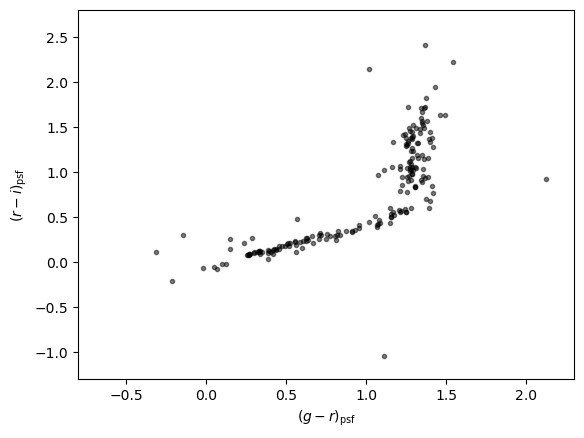
\includegraphics[keepaspectratio]{jira_imgs//zephyr0.png}}\\


}
  % end if not not executed - no steps if not executed
\paragraph{ LVV-T44 - Verify implementation of Documenting Image Characterization }\mbox{}\\

Version \textbf{1.0(d)}.
Status \textbf{Draft}.
Open  \href{https://rubinobs.atlassian.net/projects/LVV?selectedItem=com.atlassian.plugins.atlassian-connect-plugin:com.kanoah.test-manager__main-project-page\#\!/v2/testCase/LVV-T44}{\textit{ LVV-T44 } }
test case in Jira.

Verify that the persisted format for Processed Visit Images and
associated instrument-signature-removal data products is documented.

\textbf{ Preconditions}:\\ None


Execution status: {\bf Not Executed }\\
Final comment:\\None



  % end if not not executed - no steps if not executed
\paragraph{ LVV-T58 - Verify implementation of Matching DIASources to Objects }\mbox{}\\

Version \textbf{1.0(d)}.
Status \textbf{Draft}.
Open  \href{https://rubinobs.atlassian.net/projects/LVV?selectedItem=com.atlassian.plugins.atlassian-connect-plugin:com.kanoah.test-manager__main-project-page\#\!/v2/testCase/LVV-T58}{\textit{ LVV-T58 } }
test case in Jira.

Verify that a cross-match table is available between DIASources and
Objects.

\textbf{ Preconditions}:\\ None


Execution status: {\bf Not Executed }\\
Final comment:\\None



  % end if not not executed - no steps if not executed
\paragraph{ LVV-T94 - Verify implementation of Special Programs Database }\mbox{}\\

Version \textbf{1.0(d)}.
Status \textbf{Draft}.
Open  \href{https://rubinobs.atlassian.net/projects/LVV?selectedItem=com.atlassian.plugins.atlassian-connect-plugin:com.kanoah.test-manager__main-project-page\#\!/v2/testCase/LVV-T94}{\textit{ LVV-T94 } }
test case in Jira.

To confirm that data products from Special Programs are based solely on
images obtained as part of SP via, e.g., metadata queries. To confirm
that the SP data products can be joined to Prompt and DRP products by
attempting to do so via, e.g., coordinate table joins, and attempting to
e.g., find the faint counterparts in a Deep Drilling stack to variables
with no Object detections in the DRP coadds.

\textbf{ Preconditions}:\\ Databases created by reconfigured pipelines for processing Special
Programs data (e.g., DIAObject/DIASource catalogs for a Deep Drilling
Field).


Execution status: {\bf Not Executed }\\
Final comment:\\None



  % end if not not executed - no steps if not executed
\paragraph{ LVV-T56 - Verify implementation of Characterizing Variability }\mbox{}\\

Version \textbf{1.0(d)}.
Status \textbf{Draft}.
Open  \href{https://rubinobs.atlassian.net/projects/LVV?selectedItem=com.atlassian.plugins.atlassian-connect-plugin:com.kanoah.test-manager__main-project-page\#\!/v2/testCase/LVV-T56}{\textit{ LVV-T56 } }
test case in Jira.

Verify that the variability characterization in the DIAObject catalog
includes data collected within previous "diaCharacterizationCutoff"
period of time.

\textbf{ Preconditions}:\\ None


Execution status: {\bf Not Executed }\\
Final comment:\\None



  % end if not not executed - no steps if not executed
\paragraph{ LVV-T180 - Verify implementation of Data Management Unscheduled Downtime }\mbox{}\\

Version \textbf{1.0(d)}.
Status \textbf{Draft}.
Open  \href{https://rubinobs.atlassian.net/projects/LVV?selectedItem=com.atlassian.plugins.atlassian-connect-plugin:com.kanoah.test-manager__main-project-page\#\!/v2/testCase/LVV-T180}{\textit{ LVV-T180 } }
test case in Jira.

This applies only to downtime that would prevent the collection of
survey data. ~Verification means that analysis has occurred to identify
likely hardware failures that would prevent survey operations and that
mitigations that minimize the downtime to less than DMDowntime (1
day/year) are in place. ~Known systems that fall in this category
include: Image and EFD Archiving, Observatory Operations Data, Telemetry
Gateway, Data Backbone, Managed Database, Inter-Site Networks, and
Service Management and Monitoring.~

\textbf{ Preconditions}:\\ None


Execution status: {\bf Not Executed }\\
Final comment:\\None



  % end if not not executed - no steps if not executed
\paragraph{ LVV-T179 - Verify implementation of Compute Platform Heterogeneity }\mbox{}\\

Version \textbf{1.0(d)}.
Status \textbf{Draft}.
Open  \href{https://rubinobs.atlassian.net/projects/LVV?selectedItem=com.atlassian.plugins.atlassian-connect-plugin:com.kanoah.test-manager__main-project-page\#\!/v2/testCase/LVV-T179}{\textit{ LVV-T179 } }
test case in Jira.

Demonstrate that production results are the same (within machine
accuracy) when production occurs on different platforms (OS, kernel,
hardware provisioning).

\textbf{ Preconditions}:\\ None


Execution status: {\bf Not Executed }\\
Final comment:\\None



  % end if not not executed - no steps if not executed
\paragraph{ LVV-T158 - Verify implementation Level 1 and 2 Catalog Access }\mbox{}\\

Version \textbf{1.0(d)}.
Status \textbf{Draft}.
Open  \href{https://rubinobs.atlassian.net/projects/LVV?selectedItem=com.atlassian.plugins.atlassian-connect-plugin:com.kanoah.test-manager__main-project-page\#\!/v2/testCase/LVV-T158}{\textit{ LVV-T158 } }
test case in Jira.

Verify that Data Release Products are accessible by science users.

\textbf{ Preconditions}:\\ None


Execution status: {\bf Not Executed }\\
Final comment:\\None



  % end if not not executed - no steps if not executed
\paragraph{ LVV-T157 - Verify implementation Level 1 Data Product Access }\mbox{}\\

Version \textbf{1.0(d)}.
Status \textbf{Draft}.
Open  \href{https://rubinobs.atlassian.net/projects/LVV?selectedItem=com.atlassian.plugins.atlassian-connect-plugin:com.kanoah.test-manager__main-project-page\#\!/v2/testCase/LVV-T157}{\textit{ LVV-T157 } }
test case in Jira.

Verify that Level 1 Data Products are accessible by science users.

\textbf{ Preconditions}:\\ None


Execution status: {\bf Not Executed }\\
Final comment:\\None



  % end if not not executed - no steps if not executed
\paragraph{ LVV-T156 - Verify implementation of Regenerate Un-archived Data Products }\mbox{}\\

Version \textbf{1.0(d)}.
Status \textbf{Draft}.
Open  \href{https://rubinobs.atlassian.net/projects/LVV?selectedItem=com.atlassian.plugins.atlassian-connect-plugin:com.kanoah.test-manager__main-project-page\#\!/v2/testCase/LVV-T156}{\textit{ LVV-T156 } }
test case in Jira.

Not all of the ancillary data products produced by a data release will
be archived permanently. ~These ancillary products have been promised as
accessible to the community.~ Show that these products can be produced
from an archived data release after the fact.

\textbf{ Preconditions}:\\ None


Execution status: {\bf Not Executed }\\
Final comment:\\None



  % end if not not executed - no steps if not executed
\paragraph{ LVV-T155 - Verify implementation of Un-Archived Data Product Cache }\mbox{}\\

Version \textbf{1.0(d)}.
Status \textbf{Draft}.
Open  \href{https://rubinobs.atlassian.net/projects/LVV?selectedItem=com.atlassian.plugins.atlassian-connect-plugin:com.kanoah.test-manager__main-project-page\#\!/v2/testCase/LVV-T155}{\textit{ LVV-T155 } }
test case in Jira.

Demonstrate that the DMS provides low-latency storage for at least
I1CacheLifetime (30 days) to keep prompt processing pre-covery images on
hand.

\textbf{ Preconditions}:\\ None


Execution status: {\bf Not Executed }\\
Final comment:\\None



  % end if not not executed - no steps if not executed
\paragraph{ LVV-T124 - Verify implementation of Software Architecture to Enable Community
Re-Use }\mbox{}\\

Version \textbf{1.0(d)}.
Status \textbf{Defined}.
Open  \href{https://rubinobs.atlassian.net/projects/LVV?selectedItem=com.atlassian.plugins.atlassian-connect-plugin:com.kanoah.test-manager__main-project-page\#\!/v2/testCase/LVV-T124}{\textit{ LVV-T124 } }
test case in Jira.

Show that the LSST software is capable of being executed in multiple
contexts: single user instance, batch processing, continuous
integration.\\
Also show that the algorithms can be reconfigured and, if desired,
completely replaced at run time.

\textbf{ Preconditions}:\\ None


Execution status: {\bf Not Executed }\\
Final comment:\\None



  % end if not not executed - no steps if not executed
\paragraph{ LVV-T147 - Verify implementation of Control of Level-1 Production }\mbox{}\\

Version \textbf{1.0(d)}.
Status \textbf{Draft}.
Open  \href{https://rubinobs.atlassian.net/projects/LVV?selectedItem=com.atlassian.plugins.atlassian-connect-plugin:com.kanoah.test-manager__main-project-page\#\!/v2/testCase/LVV-T147}{\textit{ LVV-T147 } }
test case in Jira.

Demonstrate that the DMS can control all Prompt Processing across DMS
facilities.

\textbf{ Preconditions}:\\ None


Execution status: {\bf Not Executed }\\
Final comment:\\None



  % end if not not executed - no steps if not executed
\paragraph{ LVV-T138 - Verify provision of Bulk Download Service }\mbox{}\\

Version \textbf{1.0(d)}.
Status \textbf{Approved}.
Open  \href{https://rubinobs.atlassian.net/projects/LVV?selectedItem=com.atlassian.plugins.atlassian-connect-plugin:com.kanoah.test-manager__main-project-page\#\!/v2/testCase/LVV-T138}{\textit{ LVV-T138 } }
test case in Jira.

Verify that DM has provided software to enable bulk download of data
products andraw data, subject to network bandwidth.

\textbf{ Preconditions}:\\ 


Execution status: {\bf Pass }\\
Final comment:\\Transfers to IDACs via Rucio



% Note Steps "Not Executed" and with No Result are not shown in this report if the flag is passed
Detailed steps results LVV-R293-LVV-E3805-1319223072:\\
  {

\begin{tabular}{p{4cm}p{12cm}}
\toprule
Step LVV-E3805-1 & Step Execution Status: \textbf{ Pass } \\ \hline
\end{tabular}
 Description \\
{\footnotesize
Verify that a plan for bulk data transfer exists

}
\hdashrule[0.5ex]{\textwidth}{1pt}{3mm}
  Test Data \\
 {\footnotesize
None

}
\hdashrule[0.5ex]{\textwidth}{1pt}{3mm}
  Expected Result \\
{\footnotesize
A plan exists

}
\hdashrule[0.5ex]{\textwidth}{1pt}{3mm}
  Actual Result \\
{\footnotesize
The plans and policies for bulk data download are described in :
https://rtn-086.lsst.io/ -\/-~


}
  {

\begin{tabular}{p{4cm}p{12cm}}
\toprule
Step LVV-E3805-2 & Step Execution Status: \textbf{ Pass } \\ \hline
\end{tabular}
 Description \\
{\footnotesize
Verify that the software to enable bulk download of data products and
raw data. Exist

}
\hdashrule[0.5ex]{\textwidth}{1pt}{3mm}
  Test Data \\
 {\footnotesize
None

}
\hdashrule[0.5ex]{\textwidth}{1pt}{3mm}
  Expected Result \\
{\footnotesize
Software exists

}
\hdashrule[0.5ex]{\textwidth}{1pt}{3mm}
  Actual Result \\
{\footnotesize
The Rucio software, developed by CERN is the chosen software to enable
Rubin bulk download of data products and raw data.
https://rucio.cern.ch/ and is available in github at :
https://github.com/rucio/rucio\\
\strut \\
DM has provided additional software to add Butler specific information
to Rucio metadata: https://github.com/lsst/rucio\_register


}
  {

\begin{tabular}{p{4cm}p{12cm}}
\toprule
Step LVV-E3805-3 & Step Execution Status: \textbf{ Pass } \\ \hline
\end{tabular}
 Description \\
{\footnotesize
Inspect the logs and metrics and monitoring dashboards that demonstrate
\hspace{0pt} data transfers using the bulk data transfer service

}
\hdashrule[0.5ex]{\textwidth}{1pt}{3mm}
  Test Data \\
 {\footnotesize
None

}
\hdashrule[0.5ex]{\textwidth}{1pt}{3mm}
  Expected Result \\
{\footnotesize
Logs and monitoring of transfers available

}
\hdashrule[0.5ex]{\textwidth}{1pt}{3mm}
  Actual Result \\
{\footnotesize
A
r\href{https://grafana.slac.stanford.edu/d/YVcucApIk/rucio-transfer-monitoring?var-bin=6h&orgId=1&from=now-1Q\%2FfQ&to=now-1Q\%2FfQ&timezone=browser&var-fts=$__all&var-dst_rse=$__all&var-src_rse=$__all&var-group_by=payload.dst-rse&var-protocol=$__all&var-filters=&var-del_rse=$__all&refresh=1m}{ucio
transfer monitoring dashboard} is configured in grafana at the US data
facility and shows the transfers using Rucio. A screen shot is attached
of showing data transfers over the 3 month period from July -\/-
September 2025. The dashboard shows regular bulk data transfers to the
UK and FR data facilities of between 5-30 TB in a 1 day period.\\
\strut \\
\textbf{Image Download Error}


}
  % end if not not executed - no steps if not executed
\paragraph{ LVV-T99 - Verify implementation of Processing of Datasets }\mbox{}\\

Version \textbf{1.0(d)}.
Status \textbf{Approved}.
Open  \href{https://rubinobs.atlassian.net/projects/LVV?selectedItem=com.atlassian.plugins.atlassian-connect-plugin:com.kanoah.test-manager__main-project-page\#\!/v2/testCase/LVV-T99}{\textit{ LVV-T99 } }
test case in Jira.

Execute AP and DRP, simulate failures, observe correct processing

\textbf{ Preconditions}:\\ None


Execution status: {\bf Not Executed }\\
Final comment:\\None



  % end if not not executed - no steps if not executed
\paragraph{ LVV-T96 - Verify implementation of Query Repeatability }\mbox{}\\

Version \textbf{1.0(d)}.
Status \textbf{Draft}.
Open  \href{https://rubinobs.atlassian.net/projects/LVV?selectedItem=com.atlassian.plugins.atlassian-connect-plugin:com.kanoah.test-manager__main-project-page\#\!/v2/testCase/LVV-T96}{\textit{ LVV-T96 } }
test case in Jira.

Verify that prior queries can be rerun with identical results, or with
new additional data for live (Alert Production) databases.

\textbf{ Preconditions}:\\ None


Execution status: {\bf Not Executed }\\
Final comment:\\None



  % end if not not executed - no steps if not executed
\paragraph{ LVV-T110 - Verify implementation of DIASource Precovery }\mbox{}\\

Version \textbf{1.0(d)}.
Status \textbf{Draft}.
Open  \href{https://rubinobs.atlassian.net/projects/LVV?selectedItem=com.atlassian.plugins.atlassian-connect-plugin:com.kanoah.test-manager__main-project-page\#\!/v2/testCase/LVV-T110}{\textit{ LVV-T110 } }
test case in Jira.

Verify that DMS performs forced photometry for new DIAObjects at all
available images within the precoveryWindow.

\textbf{ Preconditions}:\\ None


Execution status: {\bf Not Executed }\\
Final comment:\\None



  % end if not not executed - no steps if not executed
\paragraph{ LVV-T108 - Verify implementation of Level 1 Source Association }\mbox{}\\

Version \textbf{1.0(d)}.
Status \textbf{Draft}.
Open  \href{https://rubinobs.atlassian.net/projects/LVV?selectedItem=com.atlassian.plugins.atlassian-connect-plugin:com.kanoah.test-manager__main-project-page\#\!/v2/testCase/LVV-T108}{\textit{ LVV-T108 } }
test case in Jira.

Verify that the DMS associates DIASources into a DIAObject or SSObject.

\textbf{ Preconditions}:\\ None


Execution status: {\bf Not Executed }\\
Final comment:\\Done for DP1 -\/- use DP1 dataset



  % end if not not executed - no steps if not executed
\paragraph{ LVV-T107 - Verify implementation of Level-1 Production Completeness }\mbox{}\\

Version \textbf{1.0(d)}.
Status \textbf{Draft}.
Open  \href{https://rubinobs.atlassian.net/projects/LVV?selectedItem=com.atlassian.plugins.atlassian-connect-plugin:com.kanoah.test-manager__main-project-page\#\!/v2/testCase/LVV-T107}{\textit{ LVV-T107 } }
test case in Jira.

Verify that the DMS successfully processes all images of sufficiently
quality for processing are eventually processed even after connectivity
failures.

\textbf{ Preconditions}:\\ None


Execution status: {\bf Not Executed }\\
Final comment:\\None



  % end if not not executed - no steps if not executed
\paragraph{ LVV-T91 - Verify implementation of Fringe Correction Frame }\mbox{}\\

Version \textbf{1.0(d)}.
Status \textbf{Approved}.
Open  \href{https://rubinobs.atlassian.net/projects/LVV?selectedItem=com.atlassian.plugins.atlassian-connect-plugin:com.kanoah.test-manager__main-project-page\#\!/v2/testCase/LVV-T91}{\textit{ LVV-T91 } }
test case in Jira.

Verify that the DMS can produce an fringe-correction frame calibration
product.\\
Verify that the DMS can determine the effectiveness of the
fringe-correction frame and determine how often it should be updated.

\textbf{ Preconditions}:\\ None


Execution status: {\bf Not Executed }\\
Final comment:\\None



  % end if not not executed - no steps if not executed
\paragraph{ LVV-T75 - Verify implementation of Multi-band Coadds }\mbox{}\\

Version \textbf{1.0(d)}.
Status \textbf{Draft}.
Open  \href{https://rubinobs.atlassian.net/projects/LVV?selectedItem=com.atlassian.plugins.atlassian-connect-plugin:com.kanoah.test-manager__main-project-page\#\!/v2/testCase/LVV-T75}{\textit{ LVV-T75 } }
test case in Jira.

Verify that the DRP pipelines produce multi-band coadds for detection
purposes.

\textbf{ Preconditions}:\\ None


Execution status: {\bf Not Executed }\\
Final comment:\\None



  % end if not not executed - no steps if not executed
\paragraph{ LVV-T74 - Verify implementation of Template Coadds }\mbox{}\\

Version \textbf{1.0(d)}.
Status \textbf{Approved}.
Open  \href{https://rubinobs.atlassian.net/projects/LVV?selectedItem=com.atlassian.plugins.atlassian-connect-plugin:com.kanoah.test-manager__main-project-page\#\!/v2/testCase/LVV-T74}{\textit{ LVV-T74 } }
test case in Jira.

Verify that the DMS can produce Template Coadds for DIA processing.

\textbf{ Preconditions}:\\ None


Execution status: {\bf Pass }\\
Final comment:\\Test executed on the RSP at USDF using pipelines version w\_2025\_33.
The executed notebook was saved in the repository associated with this
campaign's test report as ``notebooks/test\_LVV-T73.ipynb."



% Note Steps "Not Executed" and with No Result are not shown in this report if the flag is passed
Detailed steps results LVV-R293-LVV-E3813-1319223080:\\
  {

\begin{tabular}{p{4cm}p{12cm}}
\toprule
Step LVV-E3813-1 & Step Execution Status: \textbf{ Pass } \\ \hline
\end{tabular}
 Description \\
{\footnotesize
Perform the steps of Alert Production (including, but not necessarily
limited to, single frame processing, ISR, source detection/measurement,
PSF estimation, photometric and astrometric calibration, difference
imaging, DIASource detection/measurement, source association). During
Operations, it is presumed that these are automated for a given
dataset.~

}
\hdashrule[0.5ex]{\textwidth}{1pt}{3mm}
  Test Data \\
 {\footnotesize
None

}
\hdashrule[0.5ex]{\textwidth}{1pt}{3mm}
  Expected Result \\
{\footnotesize
An output dataset including difference images and DIASource and
DIAObject measurements.

}
\hdashrule[0.5ex]{\textwidth}{1pt}{3mm}
  Actual Result \\
{\footnotesize
For this test, we use the Data Preview 1 dataset as processed through
DRP processing. The butler repository and collection at USDF were
initialized as follows:\\
\strut \\
butler = Butler(\textquotesingle/repo/dp1\textquotesingle,
collections="LSSTComCam/DP1")


}
  {

\begin{tabular}{p{4cm}p{12cm}}
\toprule
Step LVV-E3813-2 & Step Execution Status: \textbf{ Pass } \\ \hline
\end{tabular}
 Description \\
{\footnotesize
Verify that the expected data products have been produced, and that
catalogs contain reasonable values for measured quantities of interest.

}
\hdashrule[0.5ex]{\textwidth}{1pt}{3mm}
  Test Data \\
 {\footnotesize
None

}
\hdashrule[0.5ex]{\textwidth}{1pt}{3mm}
  Expected Result \\
{\footnotesize

}
\hdashrule[0.5ex]{\textwidth}{1pt}{3mm}
  Actual Result \\
{\footnotesize
Catalogs are not the focus of this particular test, so we did not
examine them.


}
  {

\begin{tabular}{p{4cm}p{12cm}}
\toprule
Step LVV-E3813-3 & Step Execution Status: \textbf{ Pass } \\ \hline
\end{tabular}
 Description \\
{\footnotesize
Confirm that the template coadds have been created and are well-formed.

}
\hdashrule[0.5ex]{\textwidth}{1pt}{3mm}
  Test Data \\
 {\footnotesize
None

}
\hdashrule[0.5ex]{\textwidth}{1pt}{3mm}
  Expected Result \\
{\footnotesize

}
\hdashrule[0.5ex]{\textwidth}{1pt}{3mm}
  Actual Result \\
{\footnotesize
In the attached notebook, we displayed and examined template coadds to
confirm that they are well-formed, confirmed that the templates were
created from the 1/3 of images with the best seeing, and compared
template, visit, and difference images in the ugrizy bands.\\
\strut \\
We have confirmed that the pipelines are capable of producing and
applying well-formed template coadds.


}
  % end if not not executed - no steps if not executed
\paragraph{ LVV-T73 - Verify implementation of Deep Detection Coadds }\mbox{}\\

Version \textbf{1.0(d)}.
Status \textbf{Approved}.
Open  \href{https://rubinobs.atlassian.net/projects/LVV?selectedItem=com.atlassian.plugins.atlassian-connect-plugin:com.kanoah.test-manager__main-project-page\#\!/v2/testCase/LVV-T73}{\textit{ LVV-T73 } }
test case in Jira.

Verify that the DRP pipelines produce a suite of per-band coadded images
that are optimized for depth.

\textbf{ Preconditions}:\\ None


Execution status: {\bf Pass }\\
Final comment:\\Test executed on the RSP at USDF using pipelines version w\_2025\_33.
The executed notebook was saved in the repository associated with this
campaign's test report as ``notebooks/test\_LVV-T73.ipynb."



% Note Steps "Not Executed" and with No Result are not shown in this report if the flag is passed
Detailed steps results LVV-R293-LVV-E3814-1319223081:\\
  {

\begin{tabular}{p{4cm}p{12cm}}
\toprule
Step LVV-E3814-1 & Step Execution Status: \textbf{ Pass } \\ \hline
\end{tabular}
 Description \\
{\footnotesize
Identify the path to the data repository, which we will refer to as
\textquotesingle DATA/path\textquotesingle, then execute the following:

}
\hdashrule[0.5ex]{\textwidth}{1pt}{3mm}
  Test Data \\
 {\footnotesize
None

}
\hdashrule[0.5ex]{\textwidth}{1pt}{3mm}
  Expected Result \\
{\footnotesize
Butler repo available for reading.

}
\hdashrule[0.5ex]{\textwidth}{1pt}{3mm}
  Actual Result \\
{\footnotesize
We use data processed with w\_2025\_33, which currently resides in the
Butler repository /repo/embargo:\\
\strut \\
butler = Butler(\textquotesingle/repo/embargo\textquotesingle,
collections="LSSTCam/runs/DRP/20250604\_20250814/w\_2025\_33/DM-52202")


}
  {

\begin{tabular}{p{4cm}p{12cm}}
\toprule
Step LVV-E3814-2 & Step Execution Status: \textbf{ Pass } \\ \hline
\end{tabular}
 Description \\
{\footnotesize
Verify through inspection that per-filter coadds exist for each
tract+patch possible

}
\hdashrule[0.5ex]{\textwidth}{1pt}{3mm}
  Test Data \\
 {\footnotesize
None

}
\hdashrule[0.5ex]{\textwidth}{1pt}{3mm}
  Expected Result \\
{\footnotesize

}
\hdashrule[0.5ex]{\textwidth}{1pt}{3mm}
  Actual Result \\
{\footnotesize
In the attached notebook, we extracted the list of all visit+detector
combinations that exist in the repository. For each of these we queried
the Butler for `deep\_coadd` images overlapping the central coordinate
of the detector. All but 2\% of the visits have corresponding deep
coadds. The small fraction of images that do not have coadds likely
consists of sky areas where only a single overlapping visit was
obtained.


}
  {

\begin{tabular}{p{4cm}p{12cm}}
\toprule
Step LVV-E3814-3 & Step Execution Status: \textbf{ Pass } \\ \hline
\end{tabular}
 Description \\
{\footnotesize
Verify through inspection that the images used to generate those coadds
met specified conditions

}
\hdashrule[0.5ex]{\textwidth}{1pt}{3mm}
  Test Data \\
 {\footnotesize
None

}
\hdashrule[0.5ex]{\textwidth}{1pt}{3mm}
  Expected Result \\
{\footnotesize

}
\hdashrule[0.5ex]{\textwidth}{1pt}{3mm}
  Actual Result \\
{\footnotesize
In the attached notebook, we demonstrate that the visits contributing to
the selected i-band coadd all have seeing (measured PSF FWHM) less than
1.7", as expected. The following figure illustrates this:\\
\textbf{Image Download Error}


}
  {

\begin{tabular}{p{4cm}p{12cm}}
\toprule
Step LVV-E3814-4 & Step Execution Status: \textbf{ Pass } \\ \hline
\end{tabular}
 Description \\
{\footnotesize
Visually inspect a subset of the coadds to verify that they visually
appear reasonable and to be from good quality data.

}
\hdashrule[0.5ex]{\textwidth}{1pt}{3mm}
  Test Data \\
 {\footnotesize
None

}
\hdashrule[0.5ex]{\textwidth}{1pt}{3mm}
  Expected Result \\
{\footnotesize

}
\hdashrule[0.5ex]{\textwidth}{1pt}{3mm}
  Actual Result \\
{\footnotesize
We explored some coadd images and confirmed that they are well-formed
and reasonable. By comparison to visit images at the same position, we
also confirmed that the coadds are indeed deeper than the single-visit
images.


}
  % end if not not executed - no steps if not executed
\paragraph{ LVV-T69 - Verify implementation of Object Characterization }\mbox{}\\

Version \textbf{1.0(d)}.
Status \textbf{Draft}.
Open  \href{https://rubinobs.atlassian.net/projects/LVV?selectedItem=com.atlassian.plugins.atlassian-connect-plugin:com.kanoah.test-manager__main-project-page\#\!/v2/testCase/LVV-T69}{\textit{ LVV-T69 } }
test case in Jira.

Verify that Object catalogs produced by the DRP pipeline include all
measurements listed in DMS-REQ-0276: a point-source model fit, a
bulge-disk model fit, standard colors, a centroid, adap- tive moments,
Petrosian and Kron fluxes, surface brightness at multiple apertures,
proper motion and parallax, and a variability characterization.

\textbf{ Preconditions}:\\ None


Execution status: {\bf Not Executed }\\
Final comment:\\None



  % end if not not executed - no steps if not executed
\paragraph{ LVV-T67 - Verify implementation of Object Catalog }\mbox{}\\

Version \textbf{1.0(d)}.
Status \textbf{Draft}.
Open  \href{https://rubinobs.atlassian.net/projects/LVV?selectedItem=com.atlassian.plugins.atlassian-connect-plugin:com.kanoah.test-manager__main-project-page\#\!/v2/testCase/LVV-T67}{\textit{ LVV-T67 } }
test case in Jira.

Verify that the DRP pipelines produce an Object catalog derived from
detections made on both coadded images and difference images and
measurements performed on coadds and possibly overlapping single-epoch
images.

\textbf{ Preconditions}:\\ Input Data\\
\strut \\
DECam HiTS data (raw science images and master calibrations)\\
HSC "RC2" data (raw science images and master calibrations)


Execution status: {\bf Not Executed }\\
Final comment:\\None



  % end if not not executed - no steps if not executed
\paragraph{ LVV-T54 - Verify implementation of Alert Content }\mbox{}\\

Version \textbf{1.0(d)}.
Status \textbf{Draft}.
Open  \href{https://rubinobs.atlassian.net/projects/LVV?selectedItem=com.atlassian.plugins.atlassian-connect-plugin:com.kanoah.test-manager__main-project-page\#\!/v2/testCase/LVV-T54}{\textit{ LVV-T54 } }
test case in Jira.

Verify that the DMS creates an Alert for each detected DIASource\\
Verify that this Alert is broadcasted using community protocols\\
Verify that the context of the Alert packet match requirements.

\textbf{ Preconditions}:\\ None


Execution status: {\bf Not Executed }\\
Final comment:\\None



  % end if not not executed - no steps if not executed
\paragraph{ LVV-T52 - Verify implementation of DIAObject Attributes }\mbox{}\\

Version \textbf{1.0(d)}.
Status \textbf{Draft}.
Open  \href{https://rubinobs.atlassian.net/projects/LVV?selectedItem=com.atlassian.plugins.atlassian-connect-plugin:com.kanoah.test-manager__main-project-page\#\!/v2/testCase/LVV-T52}{\textit{ LVV-T52 } }
test case in Jira.

Verify that the DMS provides summary attributes for each DIAObject,
including periodicity measures.

\textbf{ Preconditions}:\\ None


Execution status: {\bf Not Executed }\\
Final comment:\\None



  % end if not not executed - no steps if not executed
\paragraph{ LVV-T2305 - Verify radius considered nearby }\mbox{}\\

Version \textbf{1.0(d)}.
Status \textbf{Draft}.
Open  \href{https://rubinobs.atlassian.net/projects/LVV?selectedItem=com.atlassian.plugins.atlassian-connect-plugin:com.kanoah.test-manager__main-project-page\#\!/v2/testCase/LVV-T2305}{\textit{ LVV-T2305 } }
test case in Jira.

Verify that the radius within which an Object is considered to be near,
and possibly coincident with, the DIASource is not greater that the
maximum spcification of diaNearbyObjRadius = 6 arcsec.~

\textbf{ Preconditions}:\\ None


Execution status: {\bf Not Executed }\\
Final comment:\\None



  % end if not not executed - no steps if not executed
\paragraph{ LVV-T2304 - Verify maximum number of stars associated with a DIASource. }\mbox{}\\

Version \textbf{1.0(d)}.
Status \textbf{Draft}.
Open  \href{https://rubinobs.atlassian.net/projects/LVV?selectedItem=com.atlassian.plugins.atlassian-connect-plugin:com.kanoah.test-manager__main-project-page\#\!/v2/testCase/LVV-T2304}{\textit{ LVV-T2304 } }
test case in Jira.

Verify the maximum number of stars associated with a DIASource does not
exceed the maximum of diaNearbyObjMaxStar=3

\textbf{ Preconditions}:\\ None


Execution status: {\bf Not Executed }\\
Final comment:\\None



  % end if not not executed - no steps if not executed
\paragraph{ LVV-T51 - Verify implementation of DIAObject Catalog }\mbox{}\\

Version \textbf{1.0(d)}.
Status \textbf{Draft}.
Open  \href{https://rubinobs.atlassian.net/projects/LVV?selectedItem=com.atlassian.plugins.atlassian-connect-plugin:com.kanoah.test-manager__main-project-page\#\!/v2/testCase/LVV-T51}{\textit{ LVV-T51 } }
test case in Jira.

Verify that the DIAObject includes a unique ID, identifiers for nearest
stars and nearest galaxies, and probability of matching to static
Object.

\textbf{ Preconditions}:\\ None


Execution status: {\bf Not Executed }\\
Final comment:\\None



  % end if not not executed - no steps if not executed
\paragraph{ LVV-T49 - Verify implementation of DIASource Catalog }\mbox{}\\

Version \textbf{1.0(d)}.
Status \textbf{Draft}.
Open  \href{https://rubinobs.atlassian.net/projects/LVV?selectedItem=com.atlassian.plugins.atlassian-connect-plugin:com.kanoah.test-manager__main-project-page\#\!/v2/testCase/LVV-T49}{\textit{ LVV-T49 } }
test case in Jira.

Verify that the DMS produces a Source catalog from Difference Exposures
with the required attributes.

\textbf{ Preconditions}:\\ None


Execution status: {\bf Not Executed }\\
Final comment:\\None



  % end if not not executed - no steps if not executed
\paragraph{ LVV-T65 - Verify implementation of Source Catalog }\mbox{}\\

Version \textbf{1.0(d)}.
Status \textbf{Approved}.
Open  \href{https://rubinobs.atlassian.net/projects/LVV?selectedItem=com.atlassian.plugins.atlassian-connect-plugin:com.kanoah.test-manager__main-project-page\#\!/v2/testCase/LVV-T65}{\textit{ LVV-T65 } }
test case in Jira.

Verify that all Sources produced by the DRP pipelines contain the
entries listed in DMS-REQ-0267.

\textbf{ Preconditions}:\\ None


Execution status: {\bf Pass }\\
Final comment:\\Test executed on the RSP at USDF, using pipelines version w\_2025\_33.
The executed notebook was saved in the repository associated with this
campaign's test report as ``notebooks/test\_LVV-T65.ipynb."



% Note Steps "Not Executed" and with No Result are not shown in this report if the flag is passed
Detailed steps results LVV-R293-LVV-E3823-1319223091:\\
  {

\begin{tabular}{p{4cm}p{12cm}}
\toprule
Step LVV-E3823-1 & Step Execution Status: \textbf{ Pass } \\ \hline
\end{tabular}
 Description \\
{\footnotesize
Identify a suitable small dataset to process through the DRP.

}
\hdashrule[0.5ex]{\textwidth}{1pt}{3mm}
  Test Data \\
 {\footnotesize
None

}
\hdashrule[0.5ex]{\textwidth}{1pt}{3mm}
  Expected Result \\
{\footnotesize

}
\hdashrule[0.5ex]{\textwidth}{1pt}{3mm}
  Actual Result \\
{\footnotesize
For this test, we use LSSTCam on-sky data processed in one of the
"Intermittent Cumulative DRP" campaigns.


}
  {

\begin{tabular}{p{4cm}p{12cm}}
\toprule
Step LVV-E3823-2 & Step Execution Status: \textbf{ Pass } \\ \hline
\end{tabular}
 Description \\
{\footnotesize
Process data with the Data Release Production payload, starting from raw
science images and generating science data products, placing them in the
Data Backbone.

}
\hdashrule[0.5ex]{\textwidth}{1pt}{3mm}
  Test Data \\
 {\footnotesize
None

}
\hdashrule[0.5ex]{\textwidth}{1pt}{3mm}
  Expected Result \\
{\footnotesize

}
\hdashrule[0.5ex]{\textwidth}{1pt}{3mm}
  Actual Result \\
{\footnotesize
The Butler repository and collection containing the results of the
processing was accessed via:\\
\strut \\
butler = Butler(\textquotesingle/repo/main\textquotesingle,
collections="LSSTCam/runs/DRP/20250501\_20250609/w\_2025\_30/DM-51933")


}
  {

\begin{tabular}{p{4cm}p{12cm}}
\toprule
Step LVV-E3823-3 & Step Execution Status: \textbf{ Pass } \\ \hline
\end{tabular}
 Description \\
{\footnotesize
Confirm that source catalogs have been produced for single visits and
coadds, and that it contains the required measurements.

}
\hdashrule[0.5ex]{\textwidth}{1pt}{3mm}
  Test Data \\
 {\footnotesize
None

}
\hdashrule[0.5ex]{\textwidth}{1pt}{3mm}
  Expected Result \\
{\footnotesize
A source catalog containing the measured attributes (and associated
errors), including location on the focal plane; a static point-source
model fit to world coordinates and flux; a centroid and adaptive
moments; and surface brightnesses through elliptical multiple apertures
that are concentric, PSF-homogenized, and logarithmically spaced in
intensity.

}
\hdashrule[0.5ex]{\textwidth}{1pt}{3mm}
  Actual Result \\
{\footnotesize
In the attached notebook, we demonstrate via inspection and various
plots that the required attributes are measured, and their associated
errors are provided for all sources. We note that the concentric fluxes
are measured through circular apertures, and are not PSF-homogenized,
but the scientific usefulness of such quantities is unclear. We thus
consider this a passing test, but will explore the possibility of
including additional concentric-aperture fluxes in future processing.


}
  % end if not not executed - no steps if not executed
\paragraph{ LVV-T211 - Verify implementation of Data Access Center Geographical Distribution }\mbox{}\\

Version \textbf{1.0(d)}.
Status \textbf{Approved}.
Open  \href{https://rubinobs.atlassian.net/projects/LVV?selectedItem=com.atlassian.plugins.atlassian-connect-plugin:com.kanoah.test-manager__main-project-page\#\!/v2/testCase/LVV-T211}{\textit{ LVV-T211 } }
test case in Jira.

Verify that the DACs are geographically distributed to provide
low-latency access to data-rights community.

\textbf{ Preconditions}:\\ None


Execution status: {\bf Pass }\\
Final comment:\\Setting this test case as a Pass as the Data Access Centers have long
since been established and in use since this test case was first
defined. To demonstrate the "success" of this test case, I will attach
relevant verification artifacts.



% Note Steps "Not Executed" and with No Result are not shown in this report if the flag is passed
Detailed steps results LVV-R293-LVV-E3824-1319223092:\\
  {

\begin{tabular}{p{4cm}p{12cm}}
\toprule
Step LVV-E3824-1 & Step Execution Status: \textbf{ Not Executed } \\ \hline
\end{tabular}
 Description \\
{\footnotesize
Analyze design

}
\hdashrule[0.5ex]{\textwidth}{1pt}{3mm}
  Test Data \\
 {\footnotesize
None

}
\hdashrule[0.5ex]{\textwidth}{1pt}{3mm}
  Expected Result \\
{\footnotesize

}
\hdashrule[0.5ex]{\textwidth}{1pt}{3mm}
  Actual Result \\
{\footnotesize


}
  % end if not not executed - no steps if not executed
\paragraph{ LVV-T210 - Verify implementation of Data Access Center Simultaneous Connections }\mbox{}\\

Version \textbf{1.0(d)}.
Status \textbf{Draft}.
Open  \href{https://rubinobs.atlassian.net/projects/LVV?selectedItem=com.atlassian.plugins.atlassian-connect-plugin:com.kanoah.test-manager__main-project-page\#\!/v2/testCase/LVV-T210}{\textit{ LVV-T210 } }
test case in Jira.

Verify that the each DAC can support at least dacMinConnections
simultaneously

\textbf{ Preconditions}:\\ None


Execution status: {\bf Not Executed }\\
Final comment:\\None



  % end if not not executed - no steps if not executed
\paragraph{ LVV-T209 - Verify implementation of Data Access Centers }\mbox{}\\

Version \textbf{1.0(d)}.
Status \textbf{Draft}.
Open  \href{https://rubinobs.atlassian.net/projects/LVV?selectedItem=com.atlassian.plugins.atlassian-connect-plugin:com.kanoah.test-manager__main-project-page\#\!/v2/testCase/LVV-T209}{\textit{ LVV-T209 } }
test case in Jira.

Verify that the Data Access Centers are provisioned with computing
resources necessary to support end-user access to LSST Data Products.

\textbf{ Preconditions}:\\ None


Execution status: {\bf Not Executed }\\
Final comment:\\None



  % end if not not executed - no steps if not executed
\paragraph{ LVV-T203 - Verify implementation of Archive to Data Access Center Network Secondary
Link }\mbox{}\\

Version \textbf{1.0(d)}.
Status \textbf{Draft}.
Open  \href{https://rubinobs.atlassian.net/projects/LVV?selectedItem=com.atlassian.plugins.atlassian-connect-plugin:com.kanoah.test-manager__main-project-page\#\!/v2/testCase/LVV-T203}{\textit{ LVV-T203 } }
test case in Jira.

Verify the Archive to Data Access Center Network via Secondary Link by
simulating a failure on the primary path and capacity on the secondary
path.

\textbf{ Preconditions}:\\ \begin{enumerate}
\tightlist
\item
  Data is staged in LDF and data transfer capabilities to US DAC and
  Chilean DAC are in place, running on end node computers that are the
  production hardware or equivalent to it.
\item
  As-built documentation for all of the above is available.
\end{enumerate}

NOTE: This test will be repeated at increasing data volumes as
additional observatory capabilities (e.g. ComCAM, FullCam) become
available. Final verification will be tested at full operational volume.
After the initial test, the corresponding verification elements will be
flagged as ``Requires Monitoring'' such that those requirements will be
closed out as having been verified but will continue to be monitored
throughout commissioning to ensure they do not drop out of compliance.
This will also be monitored for end to end Summit - Data Facility
transfers during Commissioning.\\
\strut \\


Execution status: {\bf Not Executed }\\
Final comment:\\None



  % end if not not executed - no steps if not executed
\paragraph{ LVV-T202 - Verify implementation of Archive to Data Access Center Network
Reliability }\mbox{}\\

Version \textbf{1.0(d)}.
Status \textbf{Draft}.
Open  \href{https://rubinobs.atlassian.net/projects/LVV?selectedItem=com.atlassian.plugins.atlassian-connect-plugin:com.kanoah.test-manager__main-project-page\#\!/v2/testCase/LVV-T202}{\textit{ LVV-T202 } }
test case in Jira.

Verify the reliability of Archive to Data Access Center Network by
demonstrating successful failover and capacity to the secondary part and
subsequent recovery to primary within or exceeding chToDacNetMTTR =
48{[}hour{]}.

\textbf{ Preconditions}:\\ \begin{enumerate}
\tightlist
\item
  Data is staged in LDF and data transfer capabilities to US DAC and
  Chilean DAC are in place, running on end node computers that are the
  production hardware or equivalent to it.
\item
  As-built documentation for all of the above is available.
\item
  NOTE: This test will be repeated at increasing data volumes as
  additional observatory capabilities (e.g. ComCAM, LSSTCam) become
  available. ~Final verification will be tested at full operational
  volume. ~After the initial test, the corresponding verification
  elements will be flagged as ``Requires Monitoring'' such that those
  requirements will be closed out as having been verified but will
  continue to be monitored throughout commissioning to ensure they do
  not drop out of compliance. This will also be monitored for end to end
  Summit - Data Facility transfers during Commissioning.
\end{enumerate}

\hfill\break


Execution status: {\bf Not Executed }\\
Final comment:\\None



  % end if not not executed - no steps if not executed
\paragraph{ LVV-T201 - Verify implementation of Archive to Data Access Center Network
Availability }\mbox{}\\

Version \textbf{1.0(d)}.
Status \textbf{Draft}.
Open  \href{https://rubinobs.atlassian.net/projects/LVV?selectedItem=com.atlassian.plugins.atlassian-connect-plugin:com.kanoah.test-manager__main-project-page\#\!/v2/testCase/LVV-T201}{\textit{ LVV-T201 } }
test case in Jira.

Verify availability of archiving to Data Access Center Network using
test and historical data of or exceeding archToDacNetMTBF= 180{[}day{]}.

\textbf{ Preconditions}:\\ \begin{enumerate}
\tightlist
\item
  Data is staged in LDF and data transfer capabilities to US DAC and
  Chilean DAC are in place, ~running on end node computers that are the
  production hardware or equivalent to it.
\item
  At least 6 months of historical monitoring data is available on these
  network links, ~running on end node computers that are the production
  hardware or equivalent to it.
\item
  As-built documentation for all of the above is available.
\end{enumerate}

NOTE: This test will be repeated at increasing data volumes as
additional observatory capabilities (e.g. ComCAM, FullCam) become
available. Final verification will be tested at full operational volume.
After the initial test, the corresponding verification elements will be
flagged as ``Requires Monitoring'' such that those requirements will be
closed out as having been verified but will continue to be monitored
throughout commissioning to ensure they do not drop out of compliance.
This will also be monitored for end to end Summit - Data Facility
transfers during Commissioning.\\
\strut \\


Execution status: {\bf Not Executed }\\
Final comment:\\None



  % end if not not executed - no steps if not executed
\paragraph{ LVV-T200 - Verify implementation of Archive to Data Access Center Network }\mbox{}\\

Version \textbf{1.0(d)}.
Status \textbf{Draft}.
Open  \href{https://rubinobs.atlassian.net/projects/LVV?selectedItem=com.atlassian.plugins.atlassian-connect-plugin:com.kanoah.test-manager__main-project-page\#\!/v2/testCase/LVV-T200}{\textit{ LVV-T200 } }
test case in Jira.

Verify archiving of data to Data Access Center Network at or exceeding
rates specified in \citeds{LDM-142}, i.e at archToDacBandwidth = 10000{[}megabit
per second{]}.

\textbf{ Preconditions}:\\ \begin{enumerate}
\tightlist
\item
  Data is staged in LDF and data transfer capabilities to US DAC and
  Chilean DAC are in place, running on end node computers that are the
  production hardware or equivalent to it.
\item
  At least 6 months of historical monitoring data is available on these
  network links.
\item
  As-built documentation for all of the above is available.
\end{enumerate}

NOTE: This test will be repeated at increasing data volumes as
additional observatory capabilities (e.g. ComCAM, LSSTCam) become
available. Final verification will be tested at full operational volume.
After the initial test, the corresponding verification elements will be
flagged as ``Requires Monitoring'' such that those requirements will be
closed out as having been verified but will continue to be monitored
throughout commissioning to ensure they do not drop out of compliance.
This will also be monitored for end to end Summit - Data Facility
transfers during Commissioning.\\
\strut \\


Execution status: {\bf Not Executed }\\
Final comment:\\None



  % end if not not executed - no steps if not executed
\paragraph{ LVV-T196 - Verify implementation of Base to Archive Network Secondary Link }\mbox{}\\

Version \textbf{1.0(d)}.
Status \textbf{Draft}.
Open  \href{https://rubinobs.atlassian.net/projects/LVV?selectedItem=com.atlassian.plugins.atlassian-connect-plugin:com.kanoah.test-manager__main-project-page\#\!/v2/testCase/LVV-T196}{\textit{ LVV-T196 } }
test case in Jira.

Verify Base to Archive Network Secondary Link failover and capacity, and
subsequent recovery primary. Demonstrate the use of the secondary path
in "catch-up" mode.

\textbf{ Preconditions}:\\ \begin{enumerate}
\tightlist
\item
  Archiver/Forwarders are configured at Base, connected to REUNA DWDM,
  loaded with simulated or pre-cursor data, running on end node
  computers that are the production hardware or equivalent to it.
\item
  Archiver/Forwarder receivers or other capability is on configured at
  LDF, connected to Base - Archive Network, running on end node
  computers that are the production hardware or equivalent to it.
\item
  As-built documentation for all of the above is available.
\end{enumerate}

NOTE: This test will be repeated at increasing data volumes as
additional observatory capabilities (e.g. ComCAM, FullCam) become
available. Final verification will be tested at full operational volume.
After the initial test, the corresponding verification elements will be
flagged as ``Requires Monitoring'' such that those requirements will be
closed out as having been verified but will continue to be monitored
throughout commissioning to ensure they do not drop out of compliance.
This will also be monitored for end to end Summit - Data Facility
transfers during Commissioning.\\
\strut \\


Execution status: {\bf Pass }\\
Final comment:\\None



% Note Steps "Not Executed" and with No Result are not shown in this report if the flag is passed
Detailed steps results LVV-R293-LVV-E3831-1319223100:\\
  {

\begin{tabular}{p{4cm}p{12cm}}
\toprule
Step LVV-E3831-1 & Step Execution Status: \textbf{ Pass } \\ \hline
\end{tabular}
 Description \\
{\footnotesize
Transfer data between base and archive on primary links over
uninterrupted 1 day period.

}
\hdashrule[0.5ex]{\textwidth}{1pt}{3mm}
  Test Data \\
 {\footnotesize
LATISS, ComCAM, or FullCAM data.

}
\hdashrule[0.5ex]{\textwidth}{1pt}{3mm}
  Expected Result \\
{\footnotesize
Data is successfully transferred over primary link at or exceeding rates
specified in LDM-142 throughout period.

}
\hdashrule[0.5ex]{\textwidth}{1pt}{3mm}
  Actual Result \\
{\footnotesize
Data is transferred succesfully\\
\strut \\
\textbf{Image Download Error}\\


}
  {

\begin{tabular}{p{4cm}p{12cm}}
\toprule
Step LVV-E3831-2 & Step Execution Status: \textbf{ Pass } \\ \hline
\end{tabular}
 Description \\
{\footnotesize
Simulate outage by disconnecting fiber on primary fiber on Base side of
Base - Archive Network.

}
\hdashrule[0.5ex]{\textwidth}{1pt}{3mm}
  Test Data \\
 {\footnotesize
NA

}
\hdashrule[0.5ex]{\textwidth}{1pt}{3mm}
  Expected Result \\
{\footnotesize
Network fails over to secondary links in \textless=60s

}
\hdashrule[0.5ex]{\textwidth}{1pt}{3mm}
  Actual Result \\
{\footnotesize
There\textquotesingle s an outage in the primary link 10/06
\textasciitilde12:00\\
\strut \\
\textbf{Image Download Error}


}
  {

\begin{tabular}{p{4cm}p{12cm}}
\toprule
Step LVV-E3831-3 & Step Execution Status: \textbf{ Pass } \\ \hline
\end{tabular}
 Description \\
{\footnotesize
Transfer data between base and archive over secondary equipment
uninterrupted 1 day period.

}
\hdashrule[0.5ex]{\textwidth}{1pt}{3mm}
  Test Data \\
 {\footnotesize
LATISS, ComCAM, or FullCAM data.

}
\hdashrule[0.5ex]{\textwidth}{1pt}{3mm}
  Expected Result \\
{\footnotesize
Data is successfully transferred over secondary link ~at or exceeding
rates specified in LDM-142 throughout period.

}
\hdashrule[0.5ex]{\textwidth}{1pt}{3mm}
  Actual Result \\
{\footnotesize
Secondary link is activated and transfers data to USDF.\\
\strut \\
\textbf{Image Download Error}


}
  {

\begin{tabular}{p{4cm}p{12cm}}
\toprule
Step LVV-E3831-4 & Step Execution Status: \textbf{ Pass } \\ \hline
\end{tabular}
 Description \\
{\footnotesize
Restore connection on primary link by reconnecting fiber.\\
\strut \\

}
\hdashrule[0.5ex]{\textwidth}{1pt}{3mm}
  Test Data \\
 {\footnotesize
NA

}
\hdashrule[0.5ex]{\textwidth}{1pt}{3mm}
  Expected Result \\
{\footnotesize
Network recovers to primary.

}
\hdashrule[0.5ex]{\textwidth}{1pt}{3mm}
  Actual Result \\
{\footnotesize
Link is recovered and data shifts to the primary link\\
\textbf{Image Download Error}\\


}
  {

\begin{tabular}{p{4cm}p{12cm}}
\toprule
Step LVV-E3831-5 & Step Execution Status: \textbf{ Pass } \\ \hline
\end{tabular}
 Description \\
{\footnotesize
Demonstrate use of secondary in catch-up mode.

}
\hdashrule[0.5ex]{\textwidth}{1pt}{3mm}
  Test Data \\
 {\footnotesize
DAQ buffer full of images and associated metadata.

}
\hdashrule[0.5ex]{\textwidth}{1pt}{3mm}
  Expected Result \\
{\footnotesize
Images from DAQ buffer and associated metadata are retrievable over
secondary path while current observing data is being transferred over
primary path.

}
\hdashrule[0.5ex]{\textwidth}{1pt}{3mm}
  Actual Result \\
{\footnotesize
Data is sent using the primery link if it\textquotesingle s available\\
\strut \\
\textbf{Image Download Error}\\


}
  % end if not not executed - no steps if not executed
\paragraph{ LVV-T195 - Verify implementation of Base to Archive Network Reliability }\mbox{}\\

Version \textbf{1.0(d)}.
Status \textbf{Draft}.
Open  \href{https://rubinobs.atlassian.net/projects/LVV?selectedItem=com.atlassian.plugins.atlassian-connect-plugin:com.kanoah.test-manager__main-project-page\#\!/v2/testCase/LVV-T195}{\textit{ LVV-T195 } }
test case in Jira.

Verify Base to Archive Network Reliability by demonstrating that the
network can recover from outages within baseToArchNetMTTR =
48{[}hour{]}.

\textbf{ Preconditions}:\\ \begin{enumerate}
\tightlist
\item
  Archiver/Forwarders are configured at Base, connected to REUNA DWDM,
  loaded with simulated or pre-cursor data, running on end node
  computers that are the production hardware or equivalent to it.
\item
  Archiver/Forwarder receivers or other capability is on configured at
  LDF, connected to Base - Archive Network, running on end node
  computers that are the production hardware or equivalent to it.
\item
  At least 6 months of monitoring data for this link is available.
\item
  As-built documentation for all of the above is available.
\end{enumerate}

NOTE: This test will be repeated at increasing data volumes as
additional observatory capabilities (e.g. ComCAM, FullCam) become
available. Final verification will be tested at full operational volume.
After the initial test, the corresponding verification elements will be
flagged as ``Requires Monitoring'' such that those requirements will be
closed out as having been verified but will continue to be monitored
throughout commissioning to ensure they do not drop out of compliance.
This will also be monitored for end to end Summit - Data Facility
transfers during Commissioning.\\
\strut \\


Execution status: {\bf Not Executed }\\
Final comment:\\None



  % end if not not executed - no steps if not executed
\paragraph{ LVV-T194 - Verify implementation of Base to Archive Network Availability }\mbox{}\\

Version \textbf{1.0(d)}.
Status \textbf{Draft}.
Open  \href{https://rubinobs.atlassian.net/projects/LVV?selectedItem=com.atlassian.plugins.atlassian-connect-plugin:com.kanoah.test-manager__main-project-page\#\!/v2/testCase/LVV-T194}{\textit{ LVV-T194 } }
test case in Jira.

Verify the availability of the Base to Archive Network communications by
demonstrating that it meets or exceeds a mean time between failures,
measured over a 1-yr period of MTBF \textgreater{} baseToArchNetMTBF
(180{[}day{]})

\textbf{ Preconditions}:\\ \begin{enumerate}
\tightlist
\item
  Archiver/Forwarders are configured at Base, connected to REUNA DWDM,
  loaded with simulated or pre-cursor data, running on end node
  computers that are the production hardware or equivalent to it.
\item
  Archiver/Forwarder receivers or other capability is on configured at
  LDF, connected to Base - Archive Network, running on end node
  computers that are the production hardware or equivalent to it.
\item
  At least 6 months of historical monitoring data on this link is
  available.
\item
  As-built documentation for all of the above is available.
\end{enumerate}

NOTE: This test will be repeated at increasing data volumes as
additional observatory capabilities (e.g. ComCAM, FullCam) become
available. Final verification will be tested at full operational volume.
After the initial test, the corresponding verification elements will be
flagged as ``Requires Monitoring'' such that those requirements will be
closed out as having been verified but will continue to be monitored
throughout commissioning to ensure they do not drop out of compliance.
This will also be monitored for end to end Summit - Data Facility
transfers during Commissioning.


Execution status: {\bf Pass }\\
Final comment:\\None



% Note Steps "Not Executed" and with No Result are not shown in this report if the flag is passed
Detailed steps results LVV-R293-LVV-E3833-1319223103:\\
  {

\begin{tabular}{p{4cm}p{12cm}}
\toprule
Step LVV-E3833-1 & Step Execution Status: \textbf{ Pass } \\ \hline
\end{tabular}
 Description \\
{\footnotesize
Transfer data between base and archive over uninterrupted 1 week period.

}
\hdashrule[0.5ex]{\textwidth}{1pt}{3mm}
  Test Data \\
 {\footnotesize
LATISS, ComCAM, or FullCAM data.

}
\hdashrule[0.5ex]{\textwidth}{1pt}{3mm}
  Expected Result \\
{\footnotesize
Data is successfully transferred during the entire week.

}
\hdashrule[0.5ex]{\textwidth}{1pt}{3mm}
  Actual Result \\
{\footnotesize
Data has been successfully transfered from Summit to USDF for several
weeks.\\
\textbf{Image Download Error}


}
  {

\begin{tabular}{p{4cm}p{12cm}}
\toprule
Step LVV-E3833-2 & Step Execution Status: \textbf{ Pass } \\ \hline
\end{tabular}
 Description \\
{\footnotesize
Analyze monitoring/performance data, compare to historical data, and
extrapolate to a full year, average and peak throughput and latency.

}
\hdashrule[0.5ex]{\textwidth}{1pt}{3mm}
  Test Data \\
 {\footnotesize
NA

}
\hdashrule[0.5ex]{\textwidth}{1pt}{3mm}
  Expected Result \\
{\footnotesize
Extrapolated network availability meets baseToArchNetMTBF =
180{[}day{]}. ~Note that this is for complete loss of transfer service
(all paths), not a single path failure with successful fail-over.

}
\hdashrule[0.5ex]{\textwidth}{1pt}{3mm}
  Actual Result \\
{\footnotesize
Since the installation of the perfsonar at SLAC (May 2024) and up to
December 2024, there has been no complete loss of transfers.\\
\textbf{Image Download Error}


}
  % end if not not executed - no steps if not executed
\paragraph{ LVV-T193 - Verify implementation of Base to Archive Network }\mbox{}\\

Version \textbf{1.0(d)}.
Status \textbf{Draft}.
Open  \href{https://rubinobs.atlassian.net/projects/LVV?selectedItem=com.atlassian.plugins.atlassian-connect-plugin:com.kanoah.test-manager__main-project-page\#\!/v2/testCase/LVV-T193}{\textit{ LVV-T193 } }
test case in Jira.

Verify that the data acquired by a DAQ can be transferred within the
required time, i.e. verify that link is capable of transferring image
for prompt processing in oArchiveMaxTransferTime = 5{[}second{]}, i.e.
at or exceeding rates specified in \citeds{LDM-142}.

\textbf{ Preconditions}:\\ \begin{enumerate}
\tightlist
\item
  Archiver/Forwarders are configured at Base, connected to REUNA DWDM,
  loaded with simulated or pre-cursor data, running on end node
  computers that are the production hardware or equivalent to it.
\item
  Archiver/Forwarder receivers or other capability is on configured at
  LDF, connected to Base - Archive Network, running on end node
  computers that are the production hardware or equivalent to it.
\item
  As-built documentation for all of the above is available.
\end{enumerate}

NOTE: This test will be repeated at increasing data volumes as
additional observatory capabilities (e.g. ComCAM, FullCam) become
available. ~Final verification will be tested at full operational
volume. After the initial test, the corresponding verification elements
will be flagged as ``Requires Monitoring'' such that those requirements
will be closed out as having been verified but will continue to be
monitored throughout commissioning to ensure they do not drop out of
compliance. This will also be monitored for end to end Summit - Data
Facility transfers during Commissioning.


Execution status: {\bf Pass }\\
Final comment:\\None



% Note Steps "Not Executed" and with No Result are not shown in this report if the flag is passed
Detailed steps results LVV-R293-LVV-E3834-1319223104:\\
  {

\begin{tabular}{p{4cm}p{12cm}}
\toprule
Step LVV-E3834-1 & Step Execution Status: \textbf{ Pass } \\ \hline
\end{tabular}
 Description \\
{\footnotesize
Transfer data between base and archive while monitoring the network over
uninterrupted 1 day period (with repeated transfers on normal observing
cadence).

}
\hdashrule[0.5ex]{\textwidth}{1pt}{3mm}
  Test Data \\
 {\footnotesize
LATISS, ComCAM, or FullCAM data.

}
\hdashrule[0.5ex]{\textwidth}{1pt}{3mm}
  Expected Result \\
{\footnotesize
Data transfers occur without significant delay or frequent latency
spikes.

}
\hdashrule[0.5ex]{\textwidth}{1pt}{3mm}
  Actual Result \\
{\footnotesize
Summit has been regularly sending ComCam data to USDF. The following is
the transfer rate of the LHN link during the first week of November
2024\\
\textbf{Image Download Error}


}
  {

\begin{tabular}{p{4cm}p{12cm}}
\toprule
Step LVV-E3834-2 & Step Execution Status: \textbf{ Pass } \\ \hline
\end{tabular}
 Description \\
{\footnotesize
~Analyze the network logs and monitoring system to determine average and
peak latency and packet loss statistics.

}
\hdashrule[0.5ex]{\textwidth}{1pt}{3mm}
  Test Data \\
 {\footnotesize
None

}
\hdashrule[0.5ex]{\textwidth}{1pt}{3mm}
  Expected Result \\
{\footnotesize
Data can be transferred within the required time, i.e. verify that link
is capable of transferring image for prompt processing in
oArchiveMaxTransferTime = 5{[}second{]}. Verify transfer of data at or
exceeding rates specified in LDM-142 at least 98\% of the time.

}
\hdashrule[0.5ex]{\textwidth}{1pt}{3mm}
  Actual Result \\
{\footnotesize
Link is capable of sending data below the 5 seconds mark. The following
is a benchmark of 10 nodes sending 25 files each of 20MB.\\
\textbf{Image Download Error}


}
  % end if not not executed - no steps if not executed
\paragraph{ LVV-T188 - Verify implementation of Summit to Base Network Ownership and Operation }\mbox{}\\

Version \textbf{1.0(d)}.
Status \textbf{Approved}.
Open  \href{https://rubinobs.atlassian.net/projects/LVV?selectedItem=com.atlassian.plugins.atlassian-connect-plugin:com.kanoah.test-manager__main-project-page\#\!/v2/testCase/LVV-T188}{\textit{ LVV-T188 } }
test case in Jira.

Verify Summit to Base Network Ownership and Operation by LSST and/or the
operations entity by inspection of construction and operations contracts
and Indefeasible Rights.

\textbf{ Preconditions}:\\ \begin{enumerate}
\tightlist
\item
  As-built documentation for all of the above contracts and IRUs is
  available.
\end{enumerate}


Execution status: {\bf Pass }\\
Final comment:\\None



% Note Steps "Not Executed" and with No Result are not shown in this report if the flag is passed
Detailed steps results LVV-R293-LVV-E3835-1319223105:\\
  {

\begin{tabular}{p{4cm}p{12cm}}
\toprule
Step LVV-E3835-1 & Step Execution Status: \textbf{ Pass } \\ \hline
\end{tabular}
 Description \\
{\footnotesize
Examine contracts with REUNA and telefonica for fiber ownership and
maintenance terms.

}
\hdashrule[0.5ex]{\textwidth}{1pt}{3mm}
  Test Data \\
 {\footnotesize
None

}
\hdashrule[0.5ex]{\textwidth}{1pt}{3mm}
  Expected Result \\
{\footnotesize
Rubin Observatory is owner of fibers on AURA property and Summit - Base
DWDM ~and has 15-year IRU for use of fibers on all segments. ~REUNA is
owner of LS - SCL DWDM on AURA property and in Santiago, and is operator
on all fibers and DWDM. ~Telefonica is contracted to maintain fibers not
on AURA property.

}
\hdashrule[0.5ex]{\textwidth}{1pt}{3mm}
  Actual Result \\
{\footnotesize
Contract CH2015-314 named "Contrato por servicio Redes de fibra óptica"
, Annex 1 specifies the following : ~"Un IRU de un enlace con ruta
diversa al canal de fibra optica de por lo menos 40Gbps por un periodo
de 15 años desde 30 de Nov. de 2019 al 30 de Sept. ~de 2034......"\\
\strut \\
In the point "Octavo" , Reuna is defined as the single responsible for
the operation and maintenance of the link.~


}
  % end if not not executed - no steps if not executed
\paragraph{ LVV-T187 - Verify implementation of Summit to Base Network Secondary Link }\mbox{}\\

Version \textbf{1.0(d)}.
Status \textbf{Draft}.
Open  \href{https://rubinobs.atlassian.net/projects/LVV?selectedItem=com.atlassian.plugins.atlassian-connect-plugin:com.kanoah.test-manager__main-project-page\#\!/v2/testCase/LVV-T187}{\textit{ LVV-T187 } }
test case in Jira.

Verify automated fail-over from primary to secondary equipment in Rubin
Observatory DWDM on simulated failure of primary. ~Verify bandwidth
sufficiency on secondary. ~Verify automated recovery to primary
equipment on simulated restoration of primary. ~Repeat for failure of
Rubin Observatory fiber and fail-over to AURA fiber and DWDM.
~Demonstrate use of secondary in "catch-up" mode.

\textbf{ Preconditions}:\\ \begin{enumerate}
\tightlist
\item
  PMCS DMTC-7400-2400 complete.
\item
  As-built documentation for Summit - Base Network is available.
\end{enumerate}

NOTE: After the initial test, the corresponding verification elements
will be flagged as ``Requires Monitoring'' such that those requirements
will be closed out as having been verified but will continue to be
monitored throughout commissioning to ensure they do not drop out of
compliance. This will also be monitored for end to end Summit - Data
Facility transfers during Commissioning.


Execution status: {\bf Not Executed }\\
Final comment:\\None



  % end if not not executed - no steps if not executed
\paragraph{ LVV-T186 - Verify implementation of Summit to Base Network Reliability }\mbox{}\\

Version \textbf{1.0(d)}.
Status \textbf{Draft}.
Open  \href{https://rubinobs.atlassian.net/projects/LVV?selectedItem=com.atlassian.plugins.atlassian-connect-plugin:com.kanoah.test-manager__main-project-page\#\!/v2/testCase/LVV-T186}{\textit{ LVV-T186 } }
test case in Jira.

Verify the reliability of the summit to base network by demonstrating
reconnection and recovery to transfer of data at or exceeding rates
specified in \citeds{LDM-142} following a cut in network connection, within MTTR
specification. The network operator will provide MTTR data on links
during commissioning and operations.\\
\strut \\

\textbf{ Preconditions}:\\ \begin{enumerate}
\tightlist
\item
  PMCS DMTC-7400-2400 Complete
\item
  As-built documentation for Summit - Base Network is available.
\end{enumerate}

NOTE: After the initial test, the corresponding verification elements
will be flagged as ``Requires Monitoring'' such that those requirements
will be closed out as having been verified but will continue to be
monitored throughout commissioning to ensure they do not drop out of
compliance. This will also be monitored for end to end Summit - Data
Facility transfers during Commissioning.


Execution status: {\bf Pass }\\
Final comment:\\None



% Note Steps "Not Executed" and with No Result are not shown in this report if the flag is passed
Detailed steps results LVV-R293-LVV-E3837-1319223109:\\
  {

\begin{tabular}{p{4cm}p{12cm}}
\toprule
Step LVV-E3837-1 & Step Execution Status: \textbf{ Pass } \\ \hline
\end{tabular}
 Description \\
{\footnotesize
Disconnect fiber cable at an endpoint location on the base side of the
Summit - Base fiber.

}
\hdashrule[0.5ex]{\textwidth}{1pt}{3mm}
  Test Data \\
 {\footnotesize
\begin{itemize}
\tightlist
\item
  LATISS, ComCAM, or LSSTCam data
\end{itemize}

}
\hdashrule[0.5ex]{\textwidth}{1pt}{3mm}
  Expected Result \\
{\footnotesize
Fiber is disconnected and the fault is detected by the network
monitoring system.

}
\hdashrule[0.5ex]{\textwidth}{1pt}{3mm}
  Actual Result \\
{\footnotesize
Fiber cut was detected and reported\\
"• Fecha y Hora de inicio: 09:04 (GMT-3), Viernes 16 de Febrero de 2024.
(Fecha del mensaje Viernes 16 de febrero de 2024, 10:06 AM)\\
• Mensaje N°: 01\\
• Descripción del problema: Informamos que detectamos
una\textbf{~falla~}en el Enlace Principal Santiago - La Serena, en el
tramo~\textbf{La Serena - Vicuña}. Ya hemos tomado contacto con
proveedor para generar un caso, saber las causas del evento y obtener
una pronta solución a este inconveniente"


}
  {

\begin{tabular}{p{4cm}p{12cm}}
\toprule
Step LVV-E3837-2 & Step Execution Status: \textbf{ Pass } \\ \hline
\end{tabular}
 Description \\
{\footnotesize
Measure the cable with the OTDR to locate the distance from the end
point. Diagnose that it is a break.

}
\hdashrule[0.5ex]{\textwidth}{1pt}{3mm}
  Test Data \\
 {\footnotesize
NA

}
\hdashrule[0.5ex]{\textwidth}{1pt}{3mm}
  Expected Result \\
{\footnotesize
OTDR shows the fiber is disconnected (break).

}
\hdashrule[0.5ex]{\textwidth}{1pt}{3mm}
  Actual Result \\
{\footnotesize
Location of the fiber cut was identified\\
"• Fecha y Hora de inicio: 09:04 (GMT-3), Viernes 16 de Febrero de 2024.
(Fecha del mensaje Viernes 16 de febrero de 2024, 12:25 PM)\\
• Mensaje N°: 04\\
• Descripción del problema: Informamos que el proveedor nos indica que
hay un corte de fibra aproximadamente 20kms de La Serena , se deben
reemplazar 400 mts de fibra un ETR de 18 hrs."


}
  {

\begin{tabular}{p{4cm}p{12cm}}
\toprule
Step LVV-E3837-3 & Step Execution Status: \textbf{ Pass } \\ \hline
\end{tabular}
 Description \\
{\footnotesize
Elapse time to simulate the following:

\begin{itemize}
\tightlist
\item
  Go to the most inaccessible place which would mean carrying all the
  tools/splicer/generator/tent equipment some ~metres.
\item
  Erect a tent to make the splice
\item
  Start the generator
\item
  Do a splice on some random piece of cable
\item
  At an end point measure the cable again to ensure it is break free.
\item
  Take down and reinstall an isolated pole (not in the actual fiber
  path)
\item
  Put the cable on the pole.
\end{itemize}

}
\hdashrule[0.5ex]{\textwidth}{1pt}{3mm}
  Test Data \\
 {\footnotesize
NA

}
\hdashrule[0.5ex]{\textwidth}{1pt}{3mm}
  Expected Result \\
{\footnotesize
Wall clock advances by 24 hours.

}
\hdashrule[0.5ex]{\textwidth}{1pt}{3mm}
  Actual Result \\
{\footnotesize
Fiber cut was detected in this location, hence a temporary tent was
built to fusion the fiber.\\
\strut \\
\textbf{Image Download Error}


}
  {

\begin{tabular}{p{4cm}p{12cm}}
\toprule
Step LVV-E3837-4 & Step Execution Status: \textbf{ Pass } \\ \hline
\end{tabular}
 Description \\
{\footnotesize
Clean fiber connections. ~Restore connection (e.g. reconnect cable).
~Cycle equipment as necessary to confirm fiber is connected.

}
\hdashrule[0.5ex]{\textwidth}{1pt}{3mm}
  Test Data \\
 {\footnotesize
NA

}
\hdashrule[0.5ex]{\textwidth}{1pt}{3mm}
  Expected Result \\
{\footnotesize
Network recovers and resumes sending data.

}
\hdashrule[0.5ex]{\textwidth}{1pt}{3mm}
  Actual Result \\
{\footnotesize
Network was recovered\\
"• Fecha y Hora de inicio: 09:04 (GMT-3), Viernes 16 de Febrero de 2024.
(Fecha del correo de finalizacion, sabado 17 de Febrero 2024, 10:43
PM)\\
• Fecha y Hora de término: 17:23 (GMT-3), Viernes 16 de Febrero de
2024\\
• Tiempo estimado de solución: Pendiente\\
• Motivo: Pendiente\\
• Mensaje N°: 08\\
• Descripción del problema: Proveedor informa que trabajos de reparación
finalizaron, por lo tanto, no se esperan nuevas interrupciones en el
servicio.\\
Saludos cordiales desde REUNA."


}
  {

\begin{tabular}{p{4cm}p{12cm}}
\toprule
Step LVV-E3837-5 & Step Execution Status: \textbf{ Pass } \\ \hline
\end{tabular}
 Description \\
{\footnotesize
Measure with OTDR to ensure back to normal state.

}
\hdashrule[0.5ex]{\textwidth}{1pt}{3mm}
  Test Data \\
 {\footnotesize
NA

}
\hdashrule[0.5ex]{\textwidth}{1pt}{3mm}
  Expected Result \\
{\footnotesize
OTDR indicates normal state.

}
\hdashrule[0.5ex]{\textwidth}{1pt}{3mm}
  Actual Result \\
{\footnotesize
Service was restored\\
"• Fecha y Hora de inicio: 09:04 (GMT-3), Viernes 16 de Febrero de 2024.
(Fecha del correo de finalizacion, sabado 17 de Febrero 2024, 10:43
PM)\\
• Fecha y Hora de término: 17:23 (GMT-3), Viernes 16 de Febrero de
2024\\
• Tiempo estimado de solución: Pendiente\\
• Motivo: Pendiente\\
• Mensaje N°: 08\\
• Descripción del problema: Proveedor informa que trabajos de reparación
finalizaron, por lo tanto, no se esperan nuevas interrupciones en el
servicio.\\
Saludos cordiales desde REUNA."


}
  % end if not not executed - no steps if not executed
\paragraph{ LVV-T185 - Verify implementation of Summit to Base Network Availability }\mbox{}\\

Version \textbf{1.0(d)}.
Status \textbf{Draft}.
Open  \href{https://rubinobs.atlassian.net/projects/LVV?selectedItem=com.atlassian.plugins.atlassian-connect-plugin:com.kanoah.test-manager__main-project-page\#\!/v2/testCase/LVV-T185}{\textit{ LVV-T185 } }
test case in Jira.

Verify the availability of Summit to Base Network by demonstrating that
the mean time between failures is less than summToBaseNetMTBF (90 days)
over 1 year.

\textbf{ Preconditions}:\\ \begin{enumerate}
\tightlist
\item
  PMCS DMTC-7400-2400 Complete.
\item
  6 months of historical availability data for this link is available.
\item
  perSonar installed in Summit and publishing statistics to MadDash.
\item
  As-built documentation for all of the above is available.
\end{enumerate}

NOTE: After the initial test, the corresponding verification elements
will be flagged as ``Requires Monitoring'' such that those requirements
will be closed out as having been verified but will continue to be
monitored throughout commissioning to ensure they do not drop out of
compliance. This will also be monitored for end to end Summit - Data
Facility transfers during Commissioning.


Execution status: {\bf Pass }\\
Final comment:\\None



% Note Steps "Not Executed" and with No Result are not shown in this report if the flag is passed
Detailed steps results LVV-R293-LVV-E3838-1319223110:\\
  {

\begin{tabular}{p{4cm}p{12cm}}
\toprule
Step LVV-E3838-1 & Step Execution Status: \textbf{ Pass } \\ \hline
\end{tabular}
 Description \\
{\footnotesize
Monitor summit to base networking for at least 1 week

}
\hdashrule[0.5ex]{\textwidth}{1pt}{3mm}
  Test Data \\
 {\footnotesize
LATISS, ComCAM, and/or Full Camera data.

}
\hdashrule[0.5ex]{\textwidth}{1pt}{3mm}
  Expected Result \\
{\footnotesize
Summit - base network is operational for 1 week and monitoring data is
collected.

}
\hdashrule[0.5ex]{\textwidth}{1pt}{3mm}
  Actual Result \\
{\footnotesize
Link meets the condition\\
\textbf{Image Download Error}\\


}
  {

\begin{tabular}{p{4cm}p{12cm}}
\toprule
Step LVV-E3838-2 & Step Execution Status: \textbf{ Pass } \\ \hline
\end{tabular}
 Description \\
{\footnotesize
Extrapolate annual availability, compare with at least 6 months of
historical data on the link.

}
\hdashrule[0.5ex]{\textwidth}{1pt}{3mm}
  Test Data \\
 {\footnotesize
Historical and current logs

}
\hdashrule[0.5ex]{\textwidth}{1pt}{3mm}
  Expected Result \\
{\footnotesize
The mean time between failures (MTBF) is projected to be less than
summToBaseNetMTBF (90 days) over 1 year.

}
\hdashrule[0.5ex]{\textwidth}{1pt}{3mm}
  Actual Result \\
{\footnotesize
Link meets the condition, during the last 6 months, there was only 1
outage. The rest are temperature related, and not the link\\
\strut \\
\textbf{Image Download Error}


}
  % end if not not executed - no steps if not executed
\paragraph{ LVV-T182 - Verify implementation of Prefer Computing and Storage Down }\mbox{}\\

Version \textbf{1.0(d)}.
Status \textbf{Draft}.
Open  \href{https://rubinobs.atlassian.net/projects/LVV?selectedItem=com.atlassian.plugins.atlassian-connect-plugin:com.kanoah.test-manager__main-project-page\#\!/v2/testCase/LVV-T182}{\textit{ LVV-T182 } }
test case in Jira.

Only build compute or storage facilities at the summit that are
justified by operational need or to prevent loss of data during
networking downtimes.

\textbf{ Preconditions}:\\ None


Execution status: {\bf Not Executed }\\
Final comment:\\None



  % end if not not executed - no steps if not executed
\paragraph{ LVV-T177 - Verify implementation of Incorporate Fault-Tolerance }\mbox{}\\

Version \textbf{1.0(d)}.
Status \textbf{Draft}.
Open  \href{https://rubinobs.atlassian.net/projects/LVV?selectedItem=com.atlassian.plugins.atlassian-connect-plugin:com.kanoah.test-manager__main-project-page\#\!/v2/testCase/LVV-T177}{\textit{ LVV-T177 } }
test case in Jira.

Demonstrate that Data Management Systems have features that prevent data
loss. ~Includes: MD5SUM/checksum verification for data transfer; RAID to
eliminate single-point disk failures; multi-site and tape for disaster
recovery of raw data; multiple site (and tape?) for backup/recovery of
Data Release products; DB transaction logging and backup to maintain DB
integrity. ~ (Note: storage to prevent loss in case of networking
failures is covered in
\href{https://jira.lsstcorp.org/secure/Tests.jspa\#/testCase/LVV-T175}{LVV-T175}
). ~~

\textbf{ Preconditions}:\\ None


Execution status: {\bf Not Executed }\\
Final comment:\\None



  % end if not not executed - no steps if not executed
\paragraph{ LVV-T176 - Verify implementation of Infrastructure Sizing for "catching up" }\mbox{}\\

Version \textbf{1.0(d)}.
Status \textbf{Draft}.
Open  \href{https://rubinobs.atlassian.net/projects/LVV?selectedItem=com.atlassian.plugins.atlassian-connect-plugin:com.kanoah.test-manager__main-project-page\#\!/v2/testCase/LVV-T176}{\textit{ LVV-T176 } }
test case in Jira.

Demonstrate Data Management System has sufficient excess capacity
(compute infrastructure) to process one night\textquotesingle s data
(2800 exposures) within 24 hours while also maintaining nightly Alert
Production (note this is very similar to
\href{https://jira.lsstcorp.org/secure/Tests.jspa\#/testCase/LVV-T173}{LVV-T173}).~

\textbf{ Preconditions}:\\ None


Execution status: {\bf Not Executed }\\
Final comment:\\None



  % end if not not executed - no steps if not executed
\paragraph{ LVV-T175 - Verify implementation of Temporary Storage for Communications Links }\mbox{}\\

Version \textbf{1.0(d)}.
Status \textbf{Draft}.
Open  \href{https://rubinobs.atlassian.net/projects/LVV?selectedItem=com.atlassian.plugins.atlassian-connect-plugin:com.kanoah.test-manager__main-project-page\#\!/v2/testCase/LVV-T175}{\textit{ LVV-T175 } }
test case in Jira.

Demonstrate that storage capacity is present and usable to prevent data
loss if networking is interrupted between summit and base, base and
archive, or archive and DAC. ~The requirement is to have storage
necessary to hold tempStorageReIMTTR (200\%) of the expected raw data
that would arrive during the Mean Time to Repair (summToBaseNetMTTR = 24
hours, baseToArchNetMTTR = 48 hours, ~archToDacNetMTTR = 48 hours).
~This scale is further set by nCalibExpDay + nRawExpNightMax = 450 +
2800 = ~3250 exposures/day.

\textbf{ Preconditions}:\\ None


Execution status: {\bf Not Executed }\\
Final comment:\\None



  % end if not not executed - no steps if not executed
\paragraph{ LVV-T174 - Verify implementation of Re-processing Capacity }\mbox{}\\

Version \textbf{1.0(d)}.
Status \textbf{Approved}.
Open  \href{https://rubinobs.atlassian.net/projects/LVV?selectedItem=com.atlassian.plugins.atlassian-connect-plugin:com.kanoah.test-manager__main-project-page\#\!/v2/testCase/LVV-T174}{\textit{ LVV-T174 } }
test case in Jira.

Verify that the DMS has sufficient processing, storage, and network to
reprocess all data within "drProcessingPeriod" (1 year) while
maintaining full Prompt Processing capability.

\textbf{ Preconditions}:\\ None


Execution status: {\bf Not Executed }\\
Final comment:\\None



  % end if not not executed - no steps if not executed
\paragraph{ LVV-T173 - Verify implementation of Pipeline Throughput }\mbox{}\\

Version \textbf{1.0(d)}.
Status \textbf{Approved}.
Open  \href{https://rubinobs.atlassian.net/projects/LVV?selectedItem=com.atlassian.plugins.atlassian-connect-plugin:com.kanoah.test-manager__main-project-page\#\!/v2/testCase/LVV-T173}{\textit{ LVV-T173 } }
test case in Jira.

Specification: The infrastructure will be sized such that the net
throughput of the data processing pipelines will permit a complete
processing of a night's observing data prior to the start of the next
observing night, assuming no system outages.\\
\strut \\
Demonstrate that the Alert Production Pipeline is capable of processing
nRawExpNightMax (2800) science exposures within a (24-nightDurationMax)
12 hour period and issue alerts in offline batch mode.~

\textbf{ Preconditions}:\\ None


Execution status: {\bf Not Executed }\\
Final comment:\\None



  % end if not not executed - no steps if not executed
\paragraph{ LVV-T172 - Verify implementation of Optimization of Cost, Reliability and
Availability }\mbox{}\\

Version \textbf{1.0(d)}.
Status \textbf{Draft}.
Open  \href{https://rubinobs.atlassian.net/projects/LVV?selectedItem=com.atlassian.plugins.atlassian-connect-plugin:com.kanoah.test-manager__main-project-page\#\!/v2/testCase/LVV-T172}{\textit{ LVV-T172 } }
test case in Jira.

In matters of cost, system reliability (functioning properly at a given
time) has precedence over system availability (ability to use the system
at a given time). ~ The optimization may be outside the realm of direct
testing as it is more of a system provisioning guideline but on its face
it demands that the Data Management System include failure reporting,
regimented change control, acceptance testing, maintenance and
monitoring.

\textbf{ Preconditions}:\\ None


Execution status: {\bf Not Executed }\\
Final comment:\\None



  % end if not not executed - no steps if not executed
\paragraph{ LVV-T131 - Verify implementation of Provide User Interface Services }\mbox{}\\

Version \textbf{1.0(d)}.
Status \textbf{Defined}.
Open  \href{https://rubinobs.atlassian.net/projects/LVV?selectedItem=com.atlassian.plugins.atlassian-connect-plugin:com.kanoah.test-manager__main-project-page\#\!/v2/testCase/LVV-T131}{\textit{ LVV-T131 } }
test case in Jira.

Verify the availability and functionality of the broad range of user
interface services called for in the requirement, as applied to both
Nightly and DRP data. ~This will primarily be done by verifications
performed at the LSST Science Platform level, based on the requirements
in \citeds{LDM-554}; however, a high-level set of tests corresponding to the
DMS-REQ-0160 requirement are defined below.

\textbf{ Preconditions}:\\ \begin{enumerate}
\tightlist
\item
  Testing this requirement relies on a set of data products meeting the
  data model implied by the DPDD existing in a deployment of the Science
  Platform and its underlying database and file services.

  \begin{enumerate}
  \tightlist
  \item
    In particular, both image and catalog data products are required.
  \item
    From the specific language of the underlying requirement, it appears
    clear that coadded data products are required, but in practice
    single-epoch data products should be included in the test as well.
  \end{enumerate}
\item
  Depending on when this requirement is tested, the tests may involve
  either or both of precursor data and LSST commissioning data. ~The use
  of the latter is ultimately essential to ensure that the tests are
  performed with as LSST-like a dataset as possible.
\end{enumerate}


Execution status: {\bf Not Executed }\\
Final comment:\\None



  % end if not not executed - no steps if not executed
\paragraph{ LVV-T64 - Verify implementation of Coadded Image Provenance }\mbox{}\\

Version \textbf{1.0(d)}.
Status \textbf{Draft}.
Open  \href{https://rubinobs.atlassian.net/projects/LVV?selectedItem=com.atlassian.plugins.atlassian-connect-plugin:com.kanoah.test-manager__main-project-page\#\!/v2/testCase/LVV-T64}{\textit{ LVV-T64 } }
test case in Jira.

Verify that all coadd data products produced by the DRP pipelines are
associated with provenance information that includes the set of input
epochs contributing to that coadd as well as any additional information
needed to exactly produce that coadd.

\textbf{ Preconditions}:\\ None


Execution status: {\bf Not Executed }\\
Final comment:\\None



  % end if not not executed - no steps if not executed
\paragraph{ LVV-T63 - Verify implementation of Produce Images for EPO }\mbox{}\\

Version \textbf{1.0(d)}.
Status \textbf{Draft}.
Open  \href{https://rubinobs.atlassian.net/projects/LVV?selectedItem=com.atlassian.plugins.atlassian-connect-plugin:com.kanoah.test-manager__main-project-page\#\!/v2/testCase/LVV-T63}{\textit{ LVV-T63 } }
test case in Jira.

This test will verify that the DRP pipelines produce the image data
products called out in \citeds{LSE-131}. ~Currently this is limited to a color
all-sky HiPS map. ~This will be verified (1) by inspection of pipeline
configurations and (2) in operations rehearsals on precursor data. ~The
production of a usable HiPS map will be verified by browsing it with
community tools.

\textbf{ Preconditions}:\\ In order for an operational test to be successful, as a precondition the
inputs to that production must exist. ~For the only currently mandated
image data production in \citeds{LSE-131}, a color all-sky HiPS map down to 1
arcsecond resolution, the prerequisite inputs to that are the
single-filter coadds in the bands required by the yet-to-be-specified
color prescription.


Execution status: {\bf Not Executed }\\
Final comment:\\None



  % end if not not executed - no steps if not executed
\paragraph{ LVV-T105 - Verify implementation of Generate Calibration Report Within Specified
Time }\mbox{}\\

Version \textbf{1.0(d)}.
Status \textbf{Draft}.
Open  \href{https://rubinobs.atlassian.net/projects/LVV?selectedItem=com.atlassian.plugins.atlassian-connect-plugin:com.kanoah.test-manager__main-project-page\#\!/v2/testCase/LVV-T105}{\textit{ LVV-T105 } }
test case in Jira.

Verify that the DMS can generate a night Calibration Report ~in both
human-readable and machine-parseable forms.

\textbf{ Preconditions}:\\ None


Execution status: {\bf Not Executed }\\
Final comment:\\None



  % end if not not executed - no steps if not executed
\paragraph{ LVV-T46 - Verify implementation of Prompt Processing Performance Report Definition }\mbox{}\\

Version \textbf{1.0(d)}.
Status \textbf{Draft}.
Open  \href{https://rubinobs.atlassian.net/projects/LVV?selectedItem=com.atlassian.plugins.atlassian-connect-plugin:com.kanoah.test-manager__main-project-page\#\!/v2/testCase/LVV-T46}{\textit{ LVV-T46 } }
test case in Jira.

Verify that the DMS produces a Prompt Processing Performance Report.
~Specifically check that the number of observations that describe each
of the following:\\
1. Successfully processed, recoverable failures, unrecoverable
failures.\\
2. Archived\\
3. Result in science.\\
\strut \\
This is testing more the processing rather than the observatory system.

\textbf{ Preconditions}:\\ None


Execution status: {\bf Not Executed }\\
Final comment:\\None



  % end if not not executed - no steps if not executed
\paragraph{ LVV-T104 - Verify implementation of Generate DMS Performance Report Within
Specified Time }\mbox{}\\

Version \textbf{1.0(d)}.
Status \textbf{Draft}.
Open  \href{https://rubinobs.atlassian.net/projects/LVV?selectedItem=com.atlassian.plugins.atlassian-connect-plugin:com.kanoah.test-manager__main-project-page\#\!/v2/testCase/LVV-T104}{\textit{ LVV-T104 } }
test case in Jira.

Verify that the DMS can generate a nightly Perfomance Report within
perfReportComplTime

\textbf{ Preconditions}:\\ None


Execution status: {\bf Not Executed }\\
Final comment:\\None



  % end if not not executed - no steps if not executed
\paragraph{ LVV-T152 - Verify implementation of Keep Historical Alert Archive }\mbox{}\\

Version \textbf{1.0(d)}.
Status \textbf{Draft}.
Open  \href{https://rubinobs.atlassian.net/projects/LVV?selectedItem=com.atlassian.plugins.atlassian-connect-plugin:com.kanoah.test-manager__main-project-page\#\!/v2/testCase/LVV-T152}{\textit{ LVV-T152 } }
test case in Jira.

Verify that the DMS preserves and makes accessible an Alert Archive for
reference and for false alert analyses

\textbf{ Preconditions}:\\ None


Execution status: {\bf Not Executed }\\
Final comment:\\None



  % end if not not executed - no steps if not executed
\paragraph{ LVV-T150 - Verify implementation of Maintain Archive Publicly Accessible }\mbox{}\\

Version \textbf{1.0(d)}.
Status \textbf{Defined}.
Open  \href{https://rubinobs.atlassian.net/projects/LVV?selectedItem=com.atlassian.plugins.atlassian-connect-plugin:com.kanoah.test-manager__main-project-page\#\!/v2/testCase/LVV-T150}{\textit{ LVV-T150 } }
test case in Jira.

Verify that prior data releases remain accessible.

\textbf{ Preconditions}:\\ Availability of at least three (3) data releases, of which at least one
of them must be archived outside the QSERV database. These can be
precursor datasets, if needed.


Execution status: {\bf Not Executed }\\
Final comment:\\None



  % end if not not executed - no steps if not executed
\paragraph{ LVV-T37 - Verify implementation of Difference Exposure Attributes }\mbox{}\\

Version \textbf{1.0(d)}.
Status \textbf{Approved}.
Open  \href{https://rubinobs.atlassian.net/projects/LVV?selectedItem=com.atlassian.plugins.atlassian-connect-plugin:com.kanoah.test-manager__main-project-page\#\!/v2/testCase/LVV-T37}{\textit{ LVV-T37 } }
test case in Jira.

Verify that for each Difference Exposure the DMS stores\\
1. The identify of the input exposures and related provenance
information\\
2. Metadata attributes of the subtraction, including the PSF-matching
kernel used.

\textbf{ Preconditions}:\\ None


Execution status: {\bf Pass }\\
Final comment:\\Test executed with pipelines version w\_2025\_41, examining data
products from w\_2025\_30 processing of LSSTCam on-sky data. The related
notebook demonstrating the detailed verification is attached to this
report\textquotesingle s github repository as test\_LVV-T37.ipynb.



% Note Steps "Not Executed" and with No Result are not shown in this report if the flag is passed
Detailed steps results LVV-R293-LVV-E3855-1319223130:\\
  {

\begin{tabular}{p{4cm}p{12cm}}
\toprule
Step LVV-E3855-1 & Step Execution Status: \textbf{ Pass } \\ \hline
\end{tabular}
 Description \\
{\footnotesize
Identify the path to the data repository, which we will refer to as
\textquotesingle DATA/path\textquotesingle, then execute the following:

}
\hdashrule[0.5ex]{\textwidth}{1pt}{3mm}
  Test Data \\
 {\footnotesize
None

}
\hdashrule[0.5ex]{\textwidth}{1pt}{3mm}
  Expected Result \\
{\footnotesize
Butler repo available for reading.

}
\hdashrule[0.5ex]{\textwidth}{1pt}{3mm}
  Actual Result \\
{\footnotesize
For this test, we use processing of LSSTCam on-sky data that included
difference imaging. The command executed to instantiate the Butler is:\\
\strut \\
```butler = Butler(\textquotesingle/repo/main\textquotesingle,
collections="LSSTCam/runs/DRP/20250501\_20250609/w\_2025\_30/DM-51933")```


}
  {

\begin{tabular}{p{4cm}p{12cm}}
\toprule
Step LVV-E3855-2 & Step Execution Status: \textbf{ Pass } \\ \hline
\end{tabular}
 Description \\
{\footnotesize
Retrieve and examine a difference image. Verify that we can recover the
provenance information about which template was used for each
subtraction, which input images were used for that template, and that we
can successfully extract the PSF matching kernel.

}
\hdashrule[0.5ex]{\textwidth}{1pt}{3mm}
  Test Data \\
 {\footnotesize
None

}
\hdashrule[0.5ex]{\textwidth}{1pt}{3mm}
  Expected Result \\
{\footnotesize

}
\hdashrule[0.5ex]{\textwidth}{1pt}{3mm}
  Actual Result \\
{\footnotesize
In the attached notebook, we demonstrate that difference images can be
retrieved for each of the ugrizy bands. An image is displayed, and it is
confirmed to be mostly blank, as expected of a difference image.\\
\strut \\
We examined the metadata, including the WCS and visitInfo, and the full
processing history.\\
\strut \\
By retrieving the `template\_detector` dataset associated with a
`difference\_image`, we confirm that the inputs that were used to create
the template can be retrieved.~\\
\strut \\
Finally, we retrieve and examine the difference kernel, an image of
which looks like the following:\\
\textbf{Image Download Error}\\
We have thus demonstrated that all of the required properties are
available with the `difference\_image` data products produced by the
LSST Science Pipelines.


}
  % end if not not executed - no steps if not executed
\paragraph{ LVV-T134 - Verify implementation of Provide Image Access Services }\mbox{}\\

Version \textbf{1.0(d)}.
Status \textbf{Draft}.
Open  \href{https://rubinobs.atlassian.net/projects/LVV?selectedItem=com.atlassian.plugins.atlassian-connect-plugin:com.kanoah.test-manager__main-project-page\#\!/v2/testCase/LVV-T134}{\textit{ LVV-T134 } }
test case in Jira.

Verify that images can be identified and that images and image cut-outs
can be retrieved using the network interfaces - primarily IVOA
standards-based - and Python APIs provided for image access by science
users.

\textbf{ Preconditions}:\\ Testing requires the establishment of running services such as SIAv2 and
SODA to which the tests can be applied.


Execution status: {\bf Not Executed }\\
Final comment:\\None



  % end if not not executed - no steps if not executed
\paragraph{ LVV-T87 - Verify implementation of Monochromatic Flatfield Data Cube }\mbox{}\\

Version \textbf{1.0(d)}.
Status \textbf{Approved}.
Open  \href{https://rubinobs.atlassian.net/projects/LVV?selectedItem=com.atlassian.plugins.atlassian-connect-plugin:com.kanoah.test-manager__main-project-page\#\!/v2/testCase/LVV-T87}{\textit{ LVV-T87 } }
test case in Jira.

Verify that the DMS can generate a calibration image/cube that corrects
for pixel-to-pixel wavelength-dependent detector response.\\
Verify that the DMS can measure the effectiveness of this monochromatic
flatfield data cube.

\textbf{ Preconditions}:\\ None


Execution status: {\bf Not Executed }\\
Final comment:\\None



  % end if not not executed - no steps if not executed
\paragraph{ LVV-T86 - Verify implementation of Illumination Correction Frame }\mbox{}\\

Version \textbf{1.0(d)}.
Status \textbf{Approved}.
Open  \href{https://rubinobs.atlassian.net/projects/LVV?selectedItem=com.atlassian.plugins.atlassian-connect-plugin:com.kanoah.test-manager__main-project-page\#\!/v2/testCase/LVV-T86}{\textit{ LVV-T86 } }
test case in Jira.

Verify that the DMS can produce an illumination correction frame
calibration product.\\
Verify that the DMS can determine the effectiveness of an illumination
correction and determine how often it should be updated.

\textbf{ Preconditions}:\\ None


Execution status: {\bf Not Executed }\\
Final comment:\\None



  % end if not not executed - no steps if not executed
\paragraph{ LVV-T130 - Verify implementation of Enable a Range of Shape Measurement Approaches }\mbox{}\\

Version \textbf{1.0(d)}.
Status \textbf{Draft}.
Open  \href{https://rubinobs.atlassian.net/projects/LVV?selectedItem=com.atlassian.plugins.atlassian-connect-plugin:com.kanoah.test-manager__main-project-page\#\!/v2/testCase/LVV-T130}{\textit{ LVV-T130 } }
test case in Jira.

Verify that multiple shape measurement algorithms can be used.

\textbf{ Preconditions}:\\ None


Execution status: {\bf Not Executed }\\
Final comment:\\None



  % end if not not executed - no steps if not executed
\paragraph{ LVV-T128 - Verify implementation Provide Astrometric Model }\mbox{}\\

Version \textbf{1.0(d)}.
Status \textbf{Draft}.
Open  \href{https://rubinobs.atlassian.net/projects/LVV?selectedItem=com.atlassian.plugins.atlassian-connect-plugin:com.kanoah.test-manager__main-project-page\#\!/v2/testCase/LVV-T128}{\textit{ LVV-T128 } }
test case in Jira.

Verify that an astrometric model is available for Objects and
DIAObjects.

\textbf{ Preconditions}:\\ None


Execution status: {\bf Not Executed }\\
Final comment:\\None



  % end if not not executed - no steps if not executed
\paragraph{ LVV-T61 - Verify implementation of Associate Sources to Objects }\mbox{}\\

Version \textbf{1.0(d)}.
Status \textbf{Defined}.
Open  \href{https://rubinobs.atlassian.net/projects/LVV?selectedItem=com.atlassian.plugins.atlassian-connect-plugin:com.kanoah.test-manager__main-project-page\#\!/v2/testCase/LVV-T61}{\textit{ LVV-T61 } }
test case in Jira.

Verify that each Source record contains an ID that associates it with a
best guess at the Object it corresponds to.

\textbf{ Preconditions}:\\ None


Execution status: {\bf Not Executed }\\
Final comment:\\None



  % end if not not executed - no steps if not executed
\paragraph{ LVV-T126 - Verify implementation of Image Differencing with coadd templates }\mbox{}\\

Version \textbf{1.0(d)}.
Status \textbf{Approved}.
Open  \href{https://rubinobs.atlassian.net/projects/LVV?selectedItem=com.atlassian.plugins.atlassian-connect-plugin:com.kanoah.test-manager__main-project-page\#\!/v2/testCase/LVV-T126}{\textit{ LVV-T126 } }
test case in Jira.

Verify that the DMS can perform image differencing from coadds.

\textbf{ Preconditions}:\\ None


Execution status: {\bf Not Executed }\\
Final comment:\\None



  % end if not not executed - no steps if not executed
\paragraph{ LVV-T171 - Verify Pipeline Availability }\mbox{}\\

Version \textbf{1.0(d)}.
Status \textbf{Defined}.
Open  \href{https://rubinobs.atlassian.net/projects/LVV?selectedItem=com.atlassian.plugins.atlassian-connect-plugin:com.kanoah.test-manager__main-project-page\#\!/v2/testCase/LVV-T171}{\textit{ LVV-T171 } }
test case in Jira.

Demonstrate that Data Management System pipelines are available for use
without disruptions of greater than productionMaxDowntime (24 hours). ~
This requires a regimented change control process and testing
infrastructure for all pipelines and their underlying software services,
and regimented management and monitoring of compute and networking
resources. ~The list of services covered by this test include: Image and
EFD Archiving, Prompt Processing, OCS Driven Batch, Telemetry Gateway,
Alert Distribution, Alert Filtering, Batch Production, Data Backbone,
Compute/Storage/LAN, Inter-Site Networks, and Service Management and
Monitoring.

\textbf{ Preconditions}:\\ None


Execution status: {\bf Not Executed }\\
Final comment:\\None



  % end if not not executed - no steps if not executed
\paragraph{ LVV-T102 - Verify implementation of Solar System Objects Available Within Specified
Time }\mbox{}\\

Version \textbf{1.0(d)}.
Status \textbf{Draft}.
Open  \href{https://rubinobs.atlassian.net/projects/LVV?selectedItem=com.atlassian.plugins.atlassian-connect-plugin:com.kanoah.test-manager__main-project-page\#\!/v2/testCase/LVV-T102}{\textit{ LVV-T102 } }
test case in Jira.

Execute single-day operations rehearsal, observe that data products for
Solar System Objects are generated in time

\textbf{ Preconditions}:\\ None


Execution status: {\bf Not Executed }\\
Final comment:\\None



  % end if not not executed - no steps if not executed
\paragraph{ LVV-T1276 - Verify implementation of latency of reporting optical transients }\mbox{}\\

Version \textbf{1.0(d)}.
Status \textbf{Draft}.
Open  \href{https://rubinobs.atlassian.net/projects/LVV?selectedItem=com.atlassian.plugins.atlassian-connect-plugin:com.kanoah.test-manager__main-project-page\#\!/v2/testCase/LVV-T1276}{\textit{ LVV-T1276 } }
test case in Jira.

Verify that alerts are generated for optical transients
within~\textbf{OTT1 = 1 minute~}of the completion of the readout of the
last image.

\textbf{ Preconditions}:\\ None


Execution status: {\bf Not Executed }\\
Final comment:\\None



  % end if not not executed - no steps if not executed
\paragraph{ LVV-T35 - Verify implementation of Nightly Data Accessible Within 24 hrs }\mbox{}\\

Version \textbf{1.0(d)}.
Status \textbf{Draft}.
Open  \href{https://rubinobs.atlassian.net/projects/LVV?selectedItem=com.atlassian.plugins.atlassian-connect-plugin:com.kanoah.test-manager__main-project-page\#\!/v2/testCase/LVV-T35}{\textit{ LVV-T35 } }
test case in Jira.

\textbf{Test Items}\\
\strut \\
Verify that\\
1. Alerts are available within OTT1\\
2. Level 1 Data Products are available within L1PublicT\\
3. Solar System Object orbits are available within L1PublicT of the
updated calculations completion on the following night.

\textbf{ Preconditions}:\\ None


Execution status: {\bf Not Executed }\\
Final comment:\\None



  % end if not not executed - no steps if not executed
\paragraph{ LVV-T95 - Verify implementation of Constraints on Level 1 Special Program Products
Generation }\mbox{}\\

Version \textbf{1.0(d)}.
Status \textbf{Draft}.
Open  \href{https://rubinobs.atlassian.net/projects/LVV?selectedItem=com.atlassian.plugins.atlassian-connect-plugin:com.kanoah.test-manager__main-project-page\#\!/v2/testCase/LVV-T95}{\textit{ LVV-T95 } }
test case in Jira.

Execute single-day operations rehearsal. Observe Prompt Processing data
products generated in time. Confirm that data from Special Programs is
processed with the same latency as required for main survey data:
release of public data within L1publicT and Alerts within OTT1.

\textbf{ Preconditions}:\\ Data from a Special Program that is appropriate for the Prompt pipeline
(i.e., a Deep Drilling type series of standard visits from a non-crowded
field).


Execution status: {\bf Not Executed }\\
Final comment:\\None



  % end if not not executed - no steps if not executed
\paragraph{ LVV-T101 - Verify implementation of Transient Alert Distribution }\mbox{}\\

Version \textbf{1.0(d)}.
Status \textbf{Approved}.
Open  \href{https://rubinobs.atlassian.net/projects/LVV?selectedItem=com.atlassian.plugins.atlassian-connect-plugin:com.kanoah.test-manager__main-project-page\#\!/v2/testCase/LVV-T101}{\textit{ LVV-T101 } }
test case in Jira.

Precursor or simulated data, execute AP, observe distribution to
simulated clients using standard protocols

\textbf{ Preconditions}:\\ 


Execution status: {\bf Pass }\\
Final comment:\\None



% Note Steps "Not Executed" and with No Result are not shown in this report if the flag is passed
Detailed steps results LVV-R293-LVV-E3868-1319223144:\\
  {

\begin{tabular}{p{4cm}p{12cm}}
\toprule
Step LVV-E3868-1 & Step Execution Status: \textbf{ Pass } \\ \hline
\end{tabular}
 Description \\
{\footnotesize
Execute AP

}
\hdashrule[0.5ex]{\textwidth}{1pt}{3mm}
  Test Data \\
 {\footnotesize
None

}
\hdashrule[0.5ex]{\textwidth}{1pt}{3mm}
  Expected Result \\
{\footnotesize

}
\hdashrule[0.5ex]{\textwidth}{1pt}{3mm}
  Actual Result \\
{\footnotesize
As of Sept. 2025 the AP pipelines are being executed during LSSTCam
on-sky observing. AP is run on images where sufficient template coverage
exists from the Science Verification survey data.


}
  {

\begin{tabular}{p{4cm}p{12cm}}
\toprule
Step LVV-E3868-2 & Step Execution Status: \textbf{ Pass } \\ \hline
\end{tabular}
 Description \\
{\footnotesize
Observe distribution to simulated clients using standard protocols

}
\hdashrule[0.5ex]{\textwidth}{1pt}{3mm}
  Test Data \\
 {\footnotesize
None

}
\hdashrule[0.5ex]{\textwidth}{1pt}{3mm}
  Expected Result \\
{\footnotesize

}
\hdashrule[0.5ex]{\textwidth}{1pt}{3mm}
  Actual Result \\
{\footnotesize
Alert distribution of LSSTCam on-sky alerts began in Sept 2025 on a
trial basis, with alerts distributed to brokers but not made publicly
visible.\\
\strut \\
The attached screenshot shows the view of an LSST alert in the Babamul
broker, demonstrating that alerts are successfully being issued by Rubin
and retrieved by brokers.\\
\strut \\
\textbf{Image Download Error}\\
Details of the Alert Distribution System can be found in
\href{https://dmtn-210.lsst.io/\#implementation-of-the-lsst-alert-distribution-system}{DMTN-210:
Implementation of the LSST Alert Distribution System}. As can be seen in
that document, the Alert Distribution System consists of a Kafka cluster
managed by Strimzi operators, a Confluent schema registry, and an alert
database that archives all alerts. These services are accessible via the
public internet by clients, who can then use the Avro schemas to decode
the alert packets that they receive.\\
\strut \\
The successful testing of alert distribution and the successful receipt
of alerts by brokers demonstrates that the Alert Distribution System is
using community standard tools that enable brokers to readily access and
ingest LSST alert packets.


}
  % end if not not executed - no steps if not executed
\paragraph{ LVV-T3103 - Verify Level 1 data product availability for transient alerts }\mbox{}\\

Version \textbf{1.0(d)}.
Status \textbf{Draft}.
Open  \href{https://rubinobs.atlassian.net/projects/LVV?selectedItem=com.atlassian.plugins.atlassian-connect-plugin:com.kanoah.test-manager__main-project-page\#\!/v2/testCase/LVV-T3103}{\textit{ LVV-T3103 } }
test case in Jira.

Verify that at least \textbf{OTR1 = 98{[}percent{]}~}of alerts are
distributed via the LSST alert distribution system within time
\textbf{OTT1 = 1{[}minute{]}~}from the conclusion of the
camera\textquotesingle s readout of the raw exposures used to generate
each alert.

\textbf{ Preconditions}:\\ None


Execution status: {\bf Not Executed }\\
Final comment:\\None



  % end if not not executed - no steps if not executed
\paragraph{ LVV-T3102 - Verify Level 1 solar system objects data product availability }\mbox{}\\

Version \textbf{1.0(d)}.
Status \textbf{Draft}.
Open  \href{https://rubinobs.atlassian.net/projects/LVV?selectedItem=com.atlassian.plugins.atlassian-connect-plugin:com.kanoah.test-manager__main-project-page\#\!/v2/testCase/LVV-T3102}{\textit{ LVV-T3102 } }
test case in Jira.

Verify that Solar System Objects are made publicly available within
\textbf{L1PublicT = 24{[}hour{]}~}of successful moving source linkage
and orbit computation.

\textbf{ Preconditions}:\\ None


Execution status: {\bf Not Executed }\\
Final comment:\\None



  % end if not not executed - no steps if not executed
\paragraph{ LVV-T3101 - Verify Level 1 data product pixel data embargo in operations }\mbox{}\\

Version \textbf{1.0(d)}.
Status \textbf{Defined}.
Open  \href{https://rubinobs.atlassian.net/projects/LVV?selectedItem=com.atlassian.plugins.atlassian-connect-plugin:com.kanoah.test-manager__main-project-page\#\!/v2/testCase/LVV-T3101}{\textit{ LVV-T3101 } }
test case in Jira.

Verify that Rubin Observatory pixel data is held in a secure location
and not released to the consortium prior to \textbf{L1EmbargoTMin =
80{[}hour{]}~}and no later than \textbf{L1EmbargoT = 81{[}hour{]}~}after
data acquisition during the Operations phase.

\textbf{ Preconditions}:\\ None


Execution status: {\bf Not Executed }\\
Final comment:\\None



  % end if not not executed - no steps if not executed
\paragraph{ LVV-T3100 - Verify secure data transfer from summit to archive }\mbox{}\\

Version \textbf{1.0(d)}.
Status \textbf{Draft}.
Open  \href{https://rubinobs.atlassian.net/projects/LVV?selectedItem=com.atlassian.plugins.atlassian-connect-plugin:com.kanoah.test-manager__main-project-page\#\!/v2/testCase/LVV-T3100}{\textit{ LVV-T3100 } }
test case in Jira.

Verify that the data transfer from the summit to the USDF complies with
funding agency requirements for cyber security.

\textbf{ Preconditions}:\\ None


Execution status: {\bf Not Executed }\\
Final comment:\\None



  % end if not not executed - no steps if not executed
\paragraph{ LVV-T3099 - Verify implementation of secure data storage }\mbox{}\\

Version \textbf{1.0(d)}.
Status \textbf{Draft}.
Open  \href{https://rubinobs.atlassian.net/projects/LVV?selectedItem=com.atlassian.plugins.atlassian-connect-plugin:com.kanoah.test-manager__main-project-page\#\!/v2/testCase/LVV-T3099}{\textit{ LVV-T3099 } }
test case in Jira.

Verify that the DMS stores image data in encrypted storage under secure
conditions with limited access to authorized staff during the period of
\textbf{L1EmbargoTmin=80{[}hour{]}}.

\textbf{ Preconditions}:\\ None


Execution status: {\bf Not Executed }\\
Final comment:\\None



  % end if not not executed - no steps if not executed
\paragraph{ LVV-T3098 - Verify uncached L1 data product lifetime for focal plane PVIs }\mbox{}\\

Version \textbf{1.0(d)}.
Status \textbf{Draft}.
Open  \href{https://rubinobs.atlassian.net/projects/LVV?selectedItem=com.atlassian.plugins.atlassian-connect-plugin:com.kanoah.test-manager__main-project-page\#\!/v2/testCase/LVV-T3098}{\textit{ LVV-T3098 } }
test case in Jira.

Verify that unarchived, Level 1 full focal-plane PVIs are available on
the file system and retrievable for \textbf{l1CacheLifetime =
30{[}day{]}.}

\textbf{ Preconditions}:\\ None


Execution status: {\bf Not Executed }\\
Final comment:\\None



  % end if not not executed - no steps if not executed
\paragraph{ LVV-T3097 - Verify the minimum number of simultaneous full-visit PVI users }\mbox{}\\

Version \textbf{1.0(d)}.
Status \textbf{Draft}.
Open  \href{https://rubinobs.atlassian.net/projects/LVV?selectedItem=com.atlassian.plugins.atlassian-connect-plugin:com.kanoah.test-manager__main-project-page\#\!/v2/testCase/LVV-T3097}{\textit{ LVV-T3097 } }
test case in Jira.

Verify that at least \textbf{allPviRetrievalUsers = 10} simultaneous
users are able to retrieve distinct focal-plane PVI datasets.\\
\strut \\
\strut \\

\textbf{ Preconditions}:\\ None


Execution status: {\bf Not Executed }\\
Final comment:\\None



  % end if not not executed - no steps if not executed
\paragraph{ LVV-T3096 - Verify uncached L1 data product lifetime for single CCDs }\mbox{}\\

Version \textbf{1.0(d)}.
Status \textbf{Draft}.
Open  \href{https://rubinobs.atlassian.net/projects/LVV?selectedItem=com.atlassian.plugins.atlassian-connect-plugin:com.kanoah.test-manager__main-project-page\#\!/v2/testCase/LVV-T3096}{\textit{ LVV-T3096 } }
test case in Jira.

Verify that unarchived, Level 1 single-CCD PVIs are available on the
file system and retrievable for \textbf{l1CacheLifetime = 30{[}day{]}.}

\textbf{ Preconditions}:\\ None


Execution status: {\bf Not Executed }\\
Final comment:\\None



  % end if not not executed - no steps if not executed
\paragraph{ LVV-T3095 - Verify the minimum number of simultaneous single-CCD PVI users }\mbox{}\\

Version \textbf{1.0(d)}.
Status \textbf{Draft}.
Open  \href{https://rubinobs.atlassian.net/projects/LVV?selectedItem=com.atlassian.plugins.atlassian-connect-plugin:com.kanoah.test-manager__main-project-page\#\!/v2/testCase/LVV-T3095}{\textit{ LVV-T3095 } }
test case in Jira.

Verify that at least \textbf{pviRetrievalUsers = 20~}simultaneous users
are able to retrieve single, distinct PVI images.

\textbf{ Preconditions}:\\ None


Execution status: {\bf Not Executed }\\
Final comment:\\None



  % end if not not executed - no steps if not executed
\paragraph{ LVV-T3094 - Verify maximum size of low-volume query results }\mbox{}\\

Version \textbf{1.0(d)}.
Status \textbf{Draft}.
Open  \href{https://rubinobs.atlassian.net/projects/LVV?selectedItem=com.atlassian.plugins.atlassian-connect-plugin:com.kanoah.test-manager__main-project-page\#\!/v2/testCase/LVV-T3094}{\textit{ LVV-T3094 } }
test case in Jira.

~Verify that low-volume queries return less than lvMaxReturnedResults =
0.5{[}gigabyte{]}~

\textbf{ Preconditions}:\\ None


Execution status: {\bf Not Executed }\\
Final comment:\\None



  % end if not not executed - no steps if not executed
\paragraph{ LVV-T60 - Publishing the Predicted Visit Schedule }\mbox{}\\

Version \textbf{1.0(d)}.
Status \textbf{Approved}.
Open  \href{https://rubinobs.atlassian.net/projects/LVV?selectedItem=com.atlassian.plugins.atlassian-connect-plugin:com.kanoah.test-manager__main-project-page\#\!/v2/testCase/LVV-T60}{\textit{ LVV-T60 } }
test case in Jira.

Verify that a predict-visit schedule can be published by the OCS.

\textbf{ Preconditions}:\\ None


Execution status: {\bf In Progress }\\
Final comment:\\None



% Note Steps "Not Executed" and with No Result are not shown in this report if the flag is passed
Detailed steps results LVV-R293-LVV-E3994-1573727255:\\
  {

\begin{tabular}{p{4cm}p{12cm}}
\toprule
Step LVV-E3994-1 & Step Execution Status: \textbf{ Pass } \\ \hline
\end{tabular}
 Description \\
{\footnotesize
Verify that a service description document exists

}
\hdashrule[0.5ex]{\textwidth}{1pt}{3mm}
  Test Data \\
 {\footnotesize
None

}
\hdashrule[0.5ex]{\textwidth}{1pt}{3mm}
  Expected Result \\
{\footnotesize
A technote describing the service exosts

}
\hdashrule[0.5ex]{\textwidth}{1pt}{3mm}
  Actual Result \\
{\footnotesize
A service description tech note exists: https://dmtn-263.lsst.io/


}
  {

\begin{tabular}{p{4cm}p{12cm}}
\toprule
Step LVV-E3994-2 & Step Execution Status: \textbf{ Pass } \\ \hline
\end{tabular}
 Description \\
{\footnotesize
Without logging on to the RSP, go to the following URL:\\
https://usdf-rsp-dev.slac.stanford.edu/obsloctap/schedule\\
\strut \\
Verify by inspection that the service is available

}
\hdashrule[0.5ex]{\textwidth}{1pt}{3mm}
  Test Data \\
 {\footnotesize
None

}
\hdashrule[0.5ex]{\textwidth}{1pt}{3mm}
  Expected Result \\
{\footnotesize
A valid webpage that shows the service~

}
\hdashrule[0.5ex]{\textwidth}{1pt}{3mm}
  Actual Result \\
{\footnotesize
The service is available as a web page~ and returns observation data
from the scheduler.~\textbf{Image Download Error}


}
  {

\begin{tabular}{p{4cm}p{12cm}}
\toprule
Step LVV-E3994-3 & Step Execution Status: \textbf{ In Progress } \\ \hline
\end{tabular}
 Description \\
{\footnotesize
Run the jupyter notebook in~\\
\strut \\
https://github.com/lsst-dm/DMTR-441/notebooks/test\_LVV-T60.ipynb

}
\hdashrule[0.5ex]{\textwidth}{1pt}{3mm}
  Test Data \\
 {\footnotesize
None

}
\hdashrule[0.5ex]{\textwidth}{1pt}{3mm}
  Expected Result \\
{\footnotesize
The notebook runs successfully. The notebook contains assertions that
check all aspects of the requirement.

}
\hdashrule[0.5ex]{\textwidth}{1pt}{3mm}
  Actual Result \\
{\footnotesize


}
  {

\begin{tabular}{p{4cm}p{12cm}}
\toprule
Step LVV-E3994-4 & Step Execution Status: \textbf{ Pass } \\ \hline
\end{tabular}
 Description \\
{\footnotesize
Verify that a user friendly UX is provided.~

}
\hdashrule[0.5ex]{\textwidth}{1pt}{3mm}
  Test Data \\
 {\footnotesize
None

}
\hdashrule[0.5ex]{\textwidth}{1pt}{3mm}
  Expected Result \\
{\footnotesize
A user-friendly user interface exists

}
\hdashrule[0.5ex]{\textwidth}{1pt}{3mm}
  Actual Result \\
{\footnotesize
A static user-friendly interface is available at:
https://usdf-rsp.slac.stanford.edu/obsloctap/static/viewer.html~ and can
be easily queries


}
  % end if not not executed - no steps if not executed
\paragraph{ LVV-T3170 - Verify max time to retrieve low-volume query results }\mbox{}\\

Version \textbf{1.0(d)}.
Status \textbf{Draft}.
Open  \href{https://rubinobs.atlassian.net/projects/LVV?selectedItem=com.atlassian.plugins.atlassian-connect-plugin:com.kanoah.test-manager__main-project-page\#\!/v2/testCase/LVV-T3170}{\textit{ LVV-T3170 } }
test case in Jira.

Verify that low volume query results are retrievable in a maximum time
of \textbf{lvQueryTime = 10 seconds.}

\textbf{ Preconditions}:\\ None


Execution status: {\bf Not Executed }\\
Final comment:\\None



  % end if not not executed - no steps if not executed
\paragraph{ LVV-T3171 - Verify min number of simultaneous low-volume query users }\mbox{}\\

Version \textbf{1.0(d)}.
Status \textbf{Draft}.
Open  \href{https://rubinobs.atlassian.net/projects/LVV?selectedItem=com.atlassian.plugins.atlassian-connect-plugin:com.kanoah.test-manager__main-project-page\#\!/v2/testCase/LVV-T3171}{\textit{ LVV-T3171 } }
test case in Jira.

Verify that a minimum of~\textbf{lvQueryUsers = 100} users can
simultaneously execute low volume queries.

\textbf{ Preconditions}:\\ None


Execution status: {\bf Not Executed }\\
Final comment:\\None



  % end if not not executed - no steps if not executed
\paragraph{ LVV-T3074 - Verify implementation of Level 1 Data Product embargo time }\mbox{}\\

Version \textbf{1.0(d)}.
Status \textbf{Draft}.
Open  \href{https://rubinobs.atlassian.net/projects/LVV?selectedItem=com.atlassian.plugins.atlassian-connect-plugin:com.kanoah.test-manager__main-project-page\#\!/v2/testCase/LVV-T3074}{\textit{ LVV-T3074 } }
test case in Jira.

Verify that Rubin Observatory visit image data is not released in any
form other than the contents of the public alert stream prior to
\textbf{L1EmbargoTMin = 80{[}hour{]}} after acquisition of the raw
image.

\textbf{ Preconditions}:\\ None


Execution status: {\bf Not Executed }\\
Final comment:\\None



  % end if not not executed - no steps if not executed
\paragraph{ LVV-T103 - Verify implementation of Generate Data Quality Report Within Specified
Time }\mbox{}\\

Version \textbf{1.0(d)}.
Status \textbf{Defined}.
Open  \href{https://rubinobs.atlassian.net/projects/LVV?selectedItem=com.atlassian.plugins.atlassian-connect-plugin:com.kanoah.test-manager__main-project-page\#\!/v2/testCase/LVV-T103}{\textit{ LVV-T103 } }
test case in Jira.

Verify that the DMS can generate a nightly L1 Data Quality Report within
\textbf{dqReportComplTime = 4{[}hour{]}}, in both human- and
machine-readable formats.

\textbf{ Preconditions}:\\ None


Execution status: {\bf Not Executed }\\
Final comment:\\None



  % end if not not executed - no steps if not executed
\paragraph{ LVV-T47 - Verify implementation of Prompt Processing Calibration Report Definition }\mbox{}\\

Version \textbf{1.0(d)}.
Status \textbf{Defined}.
Open  \href{https://rubinobs.atlassian.net/projects/LVV?selectedItem=com.atlassian.plugins.atlassian-connect-plugin:com.kanoah.test-manager__main-project-page\#\!/v2/testCase/LVV-T47}{\textit{ LVV-T47 } }
test case in Jira.

Verify that the DMS produces a Prompt Processing Calibration Report.
~Specifically check that this report is capable of identifying when
aspects of the telescope or camera are changing with time.

\textbf{ Preconditions}:\\ None


Execution status: {\bf Not Executed }\\
Final comment:\\None



  % end if not not executed - no steps if not executed
\paragraph{ LVV-T198 - Verify implementation of Archive Center Disaster Recovery }\mbox{}\\

Version \textbf{1.0(d)}.
Status \textbf{Approved}.
Open  \href{https://rubinobs.atlassian.net/projects/LVV?selectedItem=com.atlassian.plugins.atlassian-connect-plugin:com.kanoah.test-manager__main-project-page\#\!/v2/testCase/LVV-T198}{\textit{ LVV-T198 } }
test case in Jira.

Verify disaster recovery plan for Archive Center.

\textbf{ Preconditions}:\\ None


Execution status: {\bf Pass }\\
Final comment:\\None



% Note Steps "Not Executed" and with No Result are not shown in this report if the flag is passed
Detailed steps results LVV-R293-LVV-E4052-1832165345:\\
  {

\begin{tabular}{p{4cm}p{12cm}}
\toprule
Step LVV-E4052-1 & Step Execution Status: \textbf{ Pass } \\ \hline
\end{tabular}
 Description \\
{\footnotesize
Verify the existence of a disaster recovery plan for the archive center
and that it covers back up and recovery of data in teh event of a
disaster.~

}
\hdashrule[0.5ex]{\textwidth}{1pt}{3mm}
  Test Data \\
 {\footnotesize
None

}
\hdashrule[0.5ex]{\textwidth}{1pt}{3mm}
  Expected Result \\
{\footnotesize
A disaster recovery plan for the data archive exists

}
\hdashrule[0.5ex]{\textwidth}{1pt}{3mm}
  Actual Result \\
{\footnotesize
\href{http://rtn-078.lsst.io}{RTN-078}: USDF Disaster Recovery Plan,
provides the disaster recovery plan for the USDF -\/- the main
Rubin/LSST archive. ~The plan covers data recovery in the event of a
disaster for both the USDF and the cloud-based US DAC.~\\
\strut \\
It presents a risk analysis and assessment, recovery strategies for
hardware, services and data, and backup procedures.~\\

~


}
  % end if not not executed - no steps if not executed
\paragraph{ LVV-T154 - Verify implementation of Raw Data Archiving Reliability }\mbox{}\\

Version \textbf{1.0(d)}.
Status \textbf{Draft}.
Open  \href{https://rubinobs.atlassian.net/projects/LVV?selectedItem=com.atlassian.plugins.atlassian-connect-plugin:com.kanoah.test-manager__main-project-page\#\!/v2/testCase/LVV-T154}{\textit{ LVV-T154 } }
test case in Jira.

Verify that raw images are reliably archived.

\textbf{ Preconditions}:\\ None


Execution status: {\bf Not Executed }\\
Final comment:\\None



  % end if not not executed - no steps if not executed
\paragraph{ LVV-T1250 - Verify implementation of minimum number of simultaneous DM EFD query
users }\mbox{}\\

Version \textbf{1.0(d)}.
Status \textbf{Draft}.
Open  \href{https://rubinobs.atlassian.net/projects/LVV?selectedItem=com.atlassian.plugins.atlassian-connect-plugin:com.kanoah.test-manager__main-project-page\#\!/v2/testCase/LVV-T1250}{\textit{ LVV-T1250 } }
test case in Jira.

Verify that the DM EFD can support \textbf{dmEfdQueryUsers~= 5}
simultaneous queries. The additional requirement that each query must
last no more than \textbf{dmEfdQueryTime = 10 seconds~}will be verified
separately in
\href{https://jira.lsstcorp.org/secure/Tests.jspa\#/testCase/LVV-T1251}{LVV-T1251},
but these must be satisfied together.

\textbf{ Preconditions}:\\ None


Execution status: {\bf Not Executed }\\
Final comment:\\None



  % end if not not executed - no steps if not executed
\paragraph{ LVV-T1251 - Verify implementation of maximum time to retrieve DM EFD query results }\mbox{}\\

Version \textbf{1.0(d)}.
Status \textbf{Draft}.
Open  \href{https://rubinobs.atlassian.net/projects/LVV?selectedItem=com.atlassian.plugins.atlassian-connect-plugin:com.kanoah.test-manager__main-project-page\#\!/v2/testCase/LVV-T1251}{\textit{ LVV-T1251 } }
test case in Jira.

Verify that the DM EFD can support \textbf{dmEfdQueryUsers~= 5}
simultaneous queries, with each query must executing in no more than
\textbf{dmEfdQueryTime = 10 seconds.~}The requirement on at least 5
simultaneous queries will be verified separately in
\href{https://jira.lsstcorp.org/secure/Tests.jspa\#/testCase/LVV-T1250}{LVV-T1250},\href{https://jira.lsstcorp.org/secure/Tests.jspa\#/testCase/LVV-T1251}{}
but these must be satisfied together.

\textbf{ Preconditions}:\\ None


Execution status: {\bf Not Executed }\\
Final comment:\\None



  % end if not not executed - no steps if not executed
\paragraph{ LVV-T1846 - Verify calculation of band-to-band color zero-point accuracy including
u-band }\mbox{}\\

Version \textbf{1.0(d)}.
Status \textbf{Approved}.
Open  \href{https://rubinobs.atlassian.net/projects/LVV?selectedItem=com.atlassian.plugins.atlassian-connect-plugin:com.kanoah.test-manager__main-project-page\#\!/v2/testCase/LVV-T1846}{\textit{ LVV-T1846 } }
test case in Jira.

Verify that the DM system provides software to assess whether the
accuracy of absolute band-to-band color zero-points for all colors
constructed from any filter pair, including the u-band, is less than
\textbf{PA5u = 10 millimagnitudes}.

\textbf{ Preconditions}:\\ None


Execution status: {\bf Pass }\\
Final comment:\\Test performed using DRP processing of LSSTComCam data from Data Preview
1. This was necessary because there are not yet any LSSTCam observations
containing absolute flux standards in all passbands. The notebook where
calculations were performed is attached to this Report\textquotesingle s
git repository as test\_LVV-T1846.ipynb.



% Note Steps "Not Executed" and with No Result are not shown in this report if the flag is passed
Detailed steps results LVV-R293-LVV-E4057-1832165354:\\
  {

\begin{tabular}{p{4cm}p{12cm}}
\toprule
Step LVV-E4057-1 & Step Execution Status: \textbf{ Pass } \\ \hline
\end{tabular}
 Description \\
{\footnotesize
Identify spectrophotometric standard stars that have been observed as
part of a processed dataset.

}
\hdashrule[0.5ex]{\textwidth}{1pt}{3mm}
  Test Data \\
 {\footnotesize
None

}
\hdashrule[0.5ex]{\textwidth}{1pt}{3mm}
  Expected Result \\
{\footnotesize
One or more standards with well-calibrated absolute fluxes to which
measured photometry can be compared.

}
\hdashrule[0.5ex]{\textwidth}{1pt}{3mm}
  Actual Result \\
{\footnotesize
The Calspec standard C26202 was observed with LSSTComCam and was part of
Data Preview 1.


}
  {

\begin{tabular}{p{4cm}p{12cm}}
\toprule
Step LVV-E4057-2 & Step Execution Status: \textbf{ Pass } \\ \hline
\end{tabular}
 Description \\
{\footnotesize
Calculate synthetic AB magnitudes for the standard stars, using the
standard Rubin bandpasses and published Calspec (or other) SEDs.

}
\hdashrule[0.5ex]{\textwidth}{1pt}{3mm}
  Test Data \\
 {\footnotesize
None

}
\hdashrule[0.5ex]{\textwidth}{1pt}{3mm}
  Expected Result \\
{\footnotesize

}
\hdashrule[0.5ex]{\textwidth}{1pt}{3mm}
  Actual Result \\
{\footnotesize
The attached notebook demonstrates the use of the system characteristics
and throughputs from `syseng\_throughputs` to integrate the SED of
C26202 and derive magnitudes in LSSTComCam passbands.


}
  {

\begin{tabular}{p{4cm}p{12cm}}
\toprule
Step LVV-E4057-3 & Step Execution Status: \textbf{ Pass } \\ \hline
\end{tabular}
 Description \\
{\footnotesize
Extract `object` table measurements of the standards, and calculate the
median offset between the measured colors and the synthetic (predicted)
colors in the AB magnitude system. (Include only colors that contain the
u-band.) Confirm that the offsets are less than PA5u=10 mmag.

}
\hdashrule[0.5ex]{\textwidth}{1pt}{3mm}
  Test Data \\
 {\footnotesize
None

}
\hdashrule[0.5ex]{\textwidth}{1pt}{3mm}
  Expected Result \\
{\footnotesize
Median color offsets in all LSST passbands for each standard star.

}
\hdashrule[0.5ex]{\textwidth}{1pt}{3mm}
  Actual Result \\
{\footnotesize
The attached notebook compiles all measurements in each color, then
compares them to synthetic colors for C26202. Comparisons are made to
both an empirical (HST-derived) SED and a model SED from fitting to the
empirical spectrum. The offsets are as follows:\\

\begin{verbatim}

\end{verbatim}

We see that for all colors including u-band the offsets exceed the
required threshold of 10 mmag.\\
\strut \\
We have demonstrated the capability of calculating the accuracy of color
zeropoints exists. However, given that the present test was executed on
LSSTComCam data, and that the thresholds were not met, we will assess
the result as a Pass, but revisit the test when sufficient LSSTCam data
are available.


}
  % end if not not executed - no steps if not executed
\paragraph{ LVV-T1842 - Verify calculation of zeropoint error fraction exceeding the outlier
limit }\mbox{}\\

Version \textbf{1.0(d)}.
Status \textbf{Approved}.
Open  \href{https://rubinobs.atlassian.net/projects/LVV?selectedItem=com.atlassian.plugins.atlassian-connect-plugin:com.kanoah.test-manager__main-project-page\#\!/v2/testCase/LVV-T1842}{\textit{ LVV-T1842 } }
test case in Jira.

Verify that the DM system provides software to calculate the fraction of
zeropoint errors that exceed the zero point error outlier limit, and
confirm that it is less than \textbf{PF2 = 10 percent.}

\textbf{ Preconditions}:\\ None


Execution status: {\bf Pass }\\
Final comment:\\Test performed using pipelines version w\_2025\_38 and the DRP
processing of Science Validation data with pipelines version
w\_2025\_37. The notebook where calculations were performed is attached
to this Report\textquotesingle s git repository as
test\_LVV-T1842\_T2202.ipynb.



% Note Steps "Not Executed" and with No Result are not shown in this report if the flag is passed
Detailed steps results LVV-R293-LVV-E4058-1832165356:\\
  {

\begin{tabular}{p{4cm}p{12cm}}
\toprule
Step LVV-E4058-1 & Step Execution Status: \textbf{ Pass } \\ \hline
\end{tabular}
 Description \\
{\footnotesize
Identify a dataset containing at least one field in each of the u, g, r,
i, z, and y filters with multiple overlapping visits.

}
\hdashrule[0.5ex]{\textwidth}{1pt}{3mm}
  Test Data \\
 {\footnotesize
None

}
\hdashrule[0.5ex]{\textwidth}{1pt}{3mm}
  Expected Result \\
{\footnotesize
A dataset that has been ingested into a Butler repository.

}
\hdashrule[0.5ex]{\textwidth}{1pt}{3mm}
  Actual Result \\
{\footnotesize
This test used the DRP processing in Butler collection
LSSTCam/runs/DRP/20250604\_20250906/w\_2025\_37/DM-52496 of /repo/main.


}
  {

\begin{tabular}{p{4cm}p{12cm}}
\toprule
Step LVV-E4058-2 & Step Execution Status: \textbf{ Pass } \\ \hline
\end{tabular}
 Description \\
{\footnotesize
Execute `analysis\_tools` on a repository containing processed data.
Identify the path to the data, which we will call
\textquotesingle DATA/path\textquotesingle, then execute something
similar to the following (with paths, datasets, and flags replaced or
additionally specified as needed):

}
\hdashrule[0.5ex]{\textwidth}{1pt}{3mm}
  Test Data \\
 {\footnotesize
None

}
\hdashrule[0.5ex]{\textwidth}{1pt}{3mm}
  Expected Result \\
{\footnotesize
The output collection (in this case, "u/username/atools\_metrics")
containing metric measurements and any associated extras and metadata is
available via the butler.

}
\hdashrule[0.5ex]{\textwidth}{1pt}{3mm}
  Actual Result \\
{\footnotesize
While `analysis\_tools` is executed as part of DRP processing, it is not
configured to run the TargetRefcatDeltaPhotomMetrics task that
calculates the zeropoint offsets by comparing the `source` table to the
reference catalog. We thus executed the relevant tasks manually as
follows:\\
\strut \\
```\\
setup -t d\_latest lsst\_distrib\\
\strut \\
pipetask run -b /repo/main -i
LSSTCam/runs/DRP/20250604\_20250906/w\_2025\_37/DM-52496 -p
\$DRP\_PIPE\_DIR/pipelines/\_ingredients/analysis-visit-source.yaml\#makeAnalysisSourcePhotometricRefMatch,analyzeSourcePhotometricRefMatch
-o u/jcarlin/src\_refmatch\_atools\_w37 -d
"instrument=\textquotesingle LSSTCam\textquotesingle{} AND
skymap=\textquotesingle lsst\_cells\_v1\textquotesingle"
-\/-register-dataset-types -\/-instrument lsst.obs.lsst.LsstCam -j 16
2\textgreater\&1 \textbar{} tee src\_refmatch\_atools\_w37.log\\
```


}
  {

\begin{tabular}{p{4cm}p{12cm}}
\toprule
Step LVV-E4058-3 & Step Execution Status: \textbf{ Pass } \\ \hline
\end{tabular}
 Description \\
{\footnotesize
Load the relevant zeropoint metrics from the Butler repository, and
perform any calculations necessary to extract PF2.

}
\hdashrule[0.5ex]{\textwidth}{1pt}{3mm}
  Test Data \\
 {\footnotesize
None

}
\hdashrule[0.5ex]{\textwidth}{1pt}{3mm}
  Expected Result \\
{\footnotesize

}
\hdashrule[0.5ex]{\textwidth}{1pt}{3mm}
  Actual Result \\
{\footnotesize
In the attached notebook, we first queried the Butler for the relevant
datasets:\\
\strut \\
```\\
testcoll =
\textquotesingle u/jcarlin/src\_refmatch\_atools\_w37\textquotesingle{}\\
butler = Butler(\textquotesingle/repo/main\textquotesingle,
collections={[}testcoll{]})\\
srcref\_refs =
butler.query\_datasets(\textquotesingle source\_ref\_match\_photom\_metrics\textquotesingle,
collections=testcoll)\\
```\\
\strut \\
After extracting the median offsets between the source table and refcat
magnitudes, we separated them per band to make this figure:\\
\textbf{Image Download Error}


}
  {

\begin{tabular}{p{4cm}p{12cm}}
\toprule
Step LVV-E4058-4 & Step Execution Status: \textbf{ Pass } \\ \hline
\end{tabular}
 Description \\
{\footnotesize
Confirm that the PF2 value is less than 10\% for all of the ugrizy
bands.

}
\hdashrule[0.5ex]{\textwidth}{1pt}{3mm}
  Test Data \\
 {\footnotesize
None

}
\hdashrule[0.5ex]{\textwidth}{1pt}{3mm}
  Expected Result \\
{\footnotesize

}
\hdashrule[0.5ex]{\textwidth}{1pt}{3mm}
  Actual Result \\
{\footnotesize
We calculated statistics on each of the distributions from the figure
above, and found the following:\\
\strut \\

\begin{verbatim}
u band:
PF2 (outlier percentage):    0.00 %

g band:
PF2 (outlier percentage):    0.26 %

r band:
PF2 (outlier percentage):    0.21 %

i band:
PF2 (outlier percentage):    0.19 %

z band:
PF2 (outlier percentage):    0.00 %

y band:
PF2 (outlier percentage):    0.00 %
\end{verbatim}

\hfill\break
We see that the percentage of zeropoint outliers exceeding PA4=15 mmag
is less than 10\% for all of the ugrizy bands.


}
  % end if not not executed - no steps if not executed
\paragraph{ LVV-T1839 - Verify calculation of RMS width of photometric zeropoint }\mbox{}\\

Version \textbf{1.0(d)}.
Status \textbf{Approved}.
Open  \href{https://rubinobs.atlassian.net/projects/LVV?selectedItem=com.atlassian.plugins.atlassian-connect-plugin:com.kanoah.test-manager__main-project-page\#\!/v2/testCase/LVV-T1839}{\textit{ LVV-T1839 } }
test case in Jira.

Verify that the DM system provides code to assess whether the RMS width
of the internal photometric zero-point (precision of system uniformity
across the sky) for all bands except u-band is less than \textbf{PA3 =
10 millimagnitudes}.

\textbf{ Preconditions}:\\ None


Execution status: {\bf Pass }\\
Final comment:\\Test performed using pipelines version w\_2025\_38 and the DRP
processing of Science Validation data with pipelines version
w\_2025\_37. The notebook where calculations were performed is attached
to this Report\textquotesingle s git repository as
test\_LVV-T1839.ipynb.



% Note Steps "Not Executed" and with No Result are not shown in this report if the flag is passed
Detailed steps results LVV-R293-LVV-E4059-1832165358:\\
  {

\begin{tabular}{p{4cm}p{12cm}}
\toprule
Step LVV-E4059-1 & Step Execution Status: \textbf{ Pass } \\ \hline
\end{tabular}
 Description \\
{\footnotesize
Identify a dataset containing at least one field in each of the g, r, i,
z, and y filters with multiple overlapping visits.

}
\hdashrule[0.5ex]{\textwidth}{1pt}{3mm}
  Test Data \\
 {\footnotesize
None

}
\hdashrule[0.5ex]{\textwidth}{1pt}{3mm}
  Expected Result \\
{\footnotesize
A dataset that has been ingested into a Butler repository.

}
\hdashrule[0.5ex]{\textwidth}{1pt}{3mm}
  Actual Result \\
{\footnotesize
This test used the DRP processing in Butler collection
LSSTCam/runs/DRP/20250604\_20250906/w\_2025\_37/DM-52496 of /repo/main.


}
  {

\begin{tabular}{p{4cm}p{12cm}}
\toprule
Step LVV-E4059-2 & Step Execution Status: \textbf{ Pass } \\ \hline
\end{tabular}
 Description \\
{\footnotesize
Execute `analysis\_tools` on a repository containing processed data.
Identify the path to the data, which we will call
\textquotesingle DATA/path\textquotesingle, then execute something
similar to the following (with paths, datasets, and flags replaced or
additionally specified as needed):

}
\hdashrule[0.5ex]{\textwidth}{1pt}{3mm}
  Test Data \\
 {\footnotesize
None

}
\hdashrule[0.5ex]{\textwidth}{1pt}{3mm}
  Expected Result \\
{\footnotesize
The output collection (in this case, "u/username/atools\_metrics")
containing metric measurements and any associated extras and metadata is
available via the butler.

}
\hdashrule[0.5ex]{\textwidth}{1pt}{3mm}
  Actual Result \\
{\footnotesize
While `analysis\_tools` is executed as part of DRP processing, it is not
configured to run the TargetRefcatDeltaPhotomMetrics task that
calculates the zeropoint offsets by comparing the `source` table to the
reference catalog. We thus executed the relevant tasks manually as
follows:\\
\strut \\
```\\
setup -t d\_latest lsst\_distrib\\
\strut \\
pipetask run -b /repo/main -i
LSSTCam/runs/DRP/20250604\_20250906/w\_2025\_37/DM-52496 -p
\$DRP\_PIPE\_DIR/pipelines/\_ingredients/analysis-visit-source.yaml\#makeAnalysisSourcePhotometricRefMatch,analyzeSourcePhotometricRefMatch
-o u/jcarlin/src\_refmatch\_atools\_w37 -d
"instrument=\textquotesingle LSSTCam\textquotesingle{} AND
skymap=\textquotesingle lsst\_cells\_v1\textquotesingle"
-\/-register-dataset-types -\/-instrument lsst.obs.lsst.LsstCam -j 16
2\textgreater\&1 \textbar{} tee src\_refmatch\_atools\_w37.log\\
```


}
  {

\begin{tabular}{p{4cm}p{12cm}}
\toprule
Step LVV-E4059-3 & Step Execution Status: \textbf{ Pass } \\ \hline
\end{tabular}
 Description \\
{\footnotesize
Load the relevant zeropoint metrics from the Butler repository, and
perform any calculations necessary to extract PA3.

}
\hdashrule[0.5ex]{\textwidth}{1pt}{3mm}
  Test Data \\
 {\footnotesize
None

}
\hdashrule[0.5ex]{\textwidth}{1pt}{3mm}
  Expected Result \\
{\footnotesize

}
\hdashrule[0.5ex]{\textwidth}{1pt}{3mm}
  Actual Result \\
{\footnotesize
In the attached notebook, we first queried the Butler for the relevant
datasets:\\
\strut \\
```\\
testcoll =
\textquotesingle u/jcarlin/src\_refmatch\_atools\_w37\textquotesingle{}\\
butler = Butler(\textquotesingle/repo/main\textquotesingle,
collections={[}testcoll{]})\\
srcref\_refs =
butler.query\_datasets(\textquotesingle source\_ref\_match\_photom\_metrics\textquotesingle,
collections=testcoll)\\
```\\
\strut \\
After extracting the median offsets between the source table and refcat
magnitudes, we separated them per band to make this figure:\\
\textbf{Image Download Error}


}
  {

\begin{tabular}{p{4cm}p{12cm}}
\toprule
Step LVV-E4059-4 & Step Execution Status: \textbf{ Pass } \\ \hline
\end{tabular}
 Description \\
{\footnotesize
Confirm that the PA3 value is less than 10 mmag for all of the grizy
bands.

}
\hdashrule[0.5ex]{\textwidth}{1pt}{3mm}
  Test Data \\
 {\footnotesize
None

}
\hdashrule[0.5ex]{\textwidth}{1pt}{3mm}
  Expected Result \\
{\footnotesize

}
\hdashrule[0.5ex]{\textwidth}{1pt}{3mm}
  Actual Result \\
{\footnotesize
We calculated statistics on each of the distributions from the figure
above, and found the following:\\
\strut \\
\textbf{Image Download Error}\\
We see that the rms zeropoint offsets are less than 10 mmag for all five
of the grizy bands.


}
  % end if not not executed - no steps if not executed
\paragraph{ LVV-T1837 - Verify calculation of band-to-band color zero-point accuracy }\mbox{}\\

Version \textbf{1.0(d)}.
Status \textbf{Approved}.
Open  \href{https://rubinobs.atlassian.net/projects/LVV?selectedItem=com.atlassian.plugins.atlassian-connect-plugin:com.kanoah.test-manager__main-project-page\#\!/v2/testCase/LVV-T1837}{\textit{ LVV-T1837 } }
test case in Jira.

Verify that the DM system provides code to assess whether the accuracy
of absolute band-to-band color zero-points for all colors constructed
from any filter pair, excluding the u-band, is less than \textbf{PA5 = 5
millimagnitudes}.

\textbf{ Preconditions}:\\ None


Execution status: {\bf Pass }\\
Final comment:\\Test performed using DRP processing of LSSTComCam data from Data Preview
1. This was necessary because there are not yet any LSSTCam observations
containing absolute flux standards in all passbands. The notebook where
calculations were performed is attached to this Report\textquotesingle s
git repository as test\_LVV-T1837.ipynb.



% Note Steps "Not Executed" and with No Result are not shown in this report if the flag is passed
Detailed steps results LVV-R293-LVV-E4060-1832165359:\\
  {

\begin{tabular}{p{4cm}p{12cm}}
\toprule
Step LVV-E4060-1 & Step Execution Status: \textbf{ Pass } \\ \hline
\end{tabular}
 Description \\
{\footnotesize
Identify spectrophotometric standard stars that have been observed as
part of a processed dataset.

}
\hdashrule[0.5ex]{\textwidth}{1pt}{3mm}
  Test Data \\
 {\footnotesize
None

}
\hdashrule[0.5ex]{\textwidth}{1pt}{3mm}
  Expected Result \\
{\footnotesize
One or more standards with well-calibrated absolute fluxes to which
measured photometry can be compared.

}
\hdashrule[0.5ex]{\textwidth}{1pt}{3mm}
  Actual Result \\
{\footnotesize
The Calspec standard C26202 was observed with LSSTComCam and was part of
Data Preview 1.


}
  {

\begin{tabular}{p{4cm}p{12cm}}
\toprule
Step LVV-E4060-2 & Step Execution Status: \textbf{ Pass } \\ \hline
\end{tabular}
 Description \\
{\footnotesize
Calculate synthetic AB magnitudes for the standard stars, using the
standard Rubin bandpasses and published Calspec (or other) SEDs.

}
\hdashrule[0.5ex]{\textwidth}{1pt}{3mm}
  Test Data \\
 {\footnotesize
None

}
\hdashrule[0.5ex]{\textwidth}{1pt}{3mm}
  Expected Result \\
{\footnotesize

}
\hdashrule[0.5ex]{\textwidth}{1pt}{3mm}
  Actual Result \\
{\footnotesize
The attached notebook demonstrates the use of the system characteristics
and throughputs from `syseng\_throughputs` to integrate the SED of
C26202 and derive magnitudes in LSSTComCam passbands.


}
  {

\begin{tabular}{p{4cm}p{12cm}}
\toprule
Step LVV-E4060-3 & Step Execution Status: \textbf{ Pass } \\ \hline
\end{tabular}
 Description \\
{\footnotesize
Extract `object` table measurements of the standards, and calculate the
median offset between the measured colors and the synthetic (predicted)
colors in the AB magnitude system. (Include only colors without the
u-band.) Confirm that the offsets are less than PA5=5 mmag.

}
\hdashrule[0.5ex]{\textwidth}{1pt}{3mm}
  Test Data \\
 {\footnotesize
None

}
\hdashrule[0.5ex]{\textwidth}{1pt}{3mm}
  Expected Result \\
{\footnotesize
Median color offsets in all LSST passbands for each standard star.

}
\hdashrule[0.5ex]{\textwidth}{1pt}{3mm}
  Actual Result \\
{\footnotesize
The attached notebook compiles all measurements in each color, then
compares them to synthetic colors for C26202. Comparisons are made to
both an empirical (HST-derived) SED and a model SED from fitting to the
empirical spectrum. The offsets are as follows:\\

\begin{verbatim}
Image Download Error
\end{verbatim}

We see that for all colors the offsets are less than the required
threshold of 5 mmag.\\
\strut \\
We have demonstrated the capability of calculating the accuracy of color
zeropoints exists. However, given that the present test was executed on
LSSTComCam data, we will assess the result as a Pass, but revisit this
test when sufficient LSSTCam data are available.


}
  % end if not not executed - no steps if not executed
\paragraph{ LVV-T2202 - Verify that the of zero-point error outlier limit threshold (PA4) can be
applied. }\mbox{}\\

Version \textbf{1.0(d)}.
Status \textbf{Approved}.
Open  \href{https://rubinobs.atlassian.net/projects/LVV?selectedItem=com.atlassian.plugins.atlassian-connect-plugin:com.kanoah.test-manager__main-project-page\#\!/v2/testCase/LVV-T2202}{\textit{ LVV-T2202 } }
test case in Jira.

Verify that the DMS has provided the code to apply the zero-point error
outlier limit threshold (PA4) to computed values of metrics.~

\textbf{ Preconditions}:\\ None


Execution status: {\bf Pass }\\
Final comment:\\Test performed using pipelines version w\_2025\_38 and the DRP
processing of Science Validation data with pipelines version
w\_2025\_37. The notebook where calculations were performed is attached
to this Report\textquotesingle s git repository as
test\_LVV-T1842\_T2202.ipynb.



% Note Steps "Not Executed" and with No Result are not shown in this report if the flag is passed
Detailed steps results LVV-R293-LVV-E4061-1832165360:\\
  {

\begin{tabular}{p{4cm}p{12cm}}
\toprule
Step LVV-E4061-1 & Step Execution Status: \textbf{ Pass } \\ \hline
\end{tabular}
 Description \\
{\footnotesize
Identify a dataset containing at least one field in each of the u, g, r,
i, z, and y filters with multiple overlapping visits.

}
\hdashrule[0.5ex]{\textwidth}{1pt}{3mm}
  Test Data \\
 {\footnotesize
None

}
\hdashrule[0.5ex]{\textwidth}{1pt}{3mm}
  Expected Result \\
{\footnotesize
A dataset that has been ingested into a Butler repository.

}
\hdashrule[0.5ex]{\textwidth}{1pt}{3mm}
  Actual Result \\
{\footnotesize
This test used the DRP processing in Butler collection
LSSTCam/runs/DRP/20250604\_20250906/w\_2025\_37/DM-52496 of /repo/main.


}
  {

\begin{tabular}{p{4cm}p{12cm}}
\toprule
Step LVV-E4061-2 & Step Execution Status: \textbf{ Pass } \\ \hline
\end{tabular}
 Description \\
{\footnotesize
Execute `analysis\_tools` on a repository containing processed data.
Identify the path to the data, which we will call
\textquotesingle DATA/path\textquotesingle, then execute something
similar to the following (with paths, datasets, and flags replaced or
additionally specified as needed):

}
\hdashrule[0.5ex]{\textwidth}{1pt}{3mm}
  Test Data \\
 {\footnotesize
None

}
\hdashrule[0.5ex]{\textwidth}{1pt}{3mm}
  Expected Result \\
{\footnotesize
The output collection (in this case, "u/username/atools\_metrics")
containing metric measurements and any associated extras and metadata is
available via the butler.

}
\hdashrule[0.5ex]{\textwidth}{1pt}{3mm}
  Actual Result \\
{\footnotesize
While `analysis\_tools` is executed as part of DRP processing, it is not
configured to run the TargetRefcatDeltaPhotomMetrics task that
calculates the zeropoint offsets by comparing the `source` table to the
reference catalog. We thus executed the relevant tasks manually as
follows:\\
\strut \\
```\\
setup -t d\_latest lsst\_distrib\\
\strut \\
pipetask run -b /repo/main -i
LSSTCam/runs/DRP/20250604\_20250906/w\_2025\_37/DM-52496 -p
\$DRP\_PIPE\_DIR/pipelines/\_ingredients/analysis-visit-source.yaml\#makeAnalysisSourcePhotometricRefMatch,analyzeSourcePhotometricRefMatch
-o u/jcarlin/src\_refmatch\_atools\_w37 -d
"instrument=\textquotesingle LSSTCam\textquotesingle{} AND
skymap=\textquotesingle lsst\_cells\_v1\textquotesingle"
-\/-register-dataset-types -\/-instrument lsst.obs.lsst.LsstCam -j 16
2\textgreater\&1 \textbar{} tee src\_refmatch\_atools\_w37.log\\
```


}
  {

\begin{tabular}{p{4cm}p{12cm}}
\toprule
Step LVV-E4061-3 & Step Execution Status: \textbf{ Pass } \\ \hline
\end{tabular}
 Description \\
{\footnotesize
Load the relevant zeropoint metrics from the Butler repository, and
perform any calculations necessary to extract PF2 via application of the
PA4 threshold.

}
\hdashrule[0.5ex]{\textwidth}{1pt}{3mm}
  Test Data \\
 {\footnotesize
None

}
\hdashrule[0.5ex]{\textwidth}{1pt}{3mm}
  Expected Result \\
{\footnotesize

}
\hdashrule[0.5ex]{\textwidth}{1pt}{3mm}
  Actual Result \\
{\footnotesize
In the attached notebook, we first queried the Butler for the relevant
datasets:\\
\strut \\
```\\
testcoll =
\textquotesingle u/jcarlin/src\_refmatch\_atools\_w37\textquotesingle{}\\
butler = Butler(\textquotesingle/repo/main\textquotesingle,
collections={[}testcoll{]})\\
srcref\_refs =
butler.query\_datasets(\textquotesingle source\_ref\_match\_photom\_metrics\textquotesingle,
collections=testcoll)\\
```\\
\strut \\
After extracting the median offsets between the source table and refcat
magnitudes, we separated them per band to make this figure:\\
\textbf{Image Download Error}\\
\strut \\
Note that the threshold value for PA4 is overplotted on the figure.


}
  {

\begin{tabular}{p{4cm}p{12cm}}
\toprule
Step LVV-E4061-4 & Step Execution Status: \textbf{ Pass } \\ \hline
\end{tabular}
 Description \\
{\footnotesize
Confirm that the PA4 = 15 mmag threshold has been applied to enable
calculation of PF2.

}
\hdashrule[0.5ex]{\textwidth}{1pt}{3mm}
  Test Data \\
 {\footnotesize
None

}
\hdashrule[0.5ex]{\textwidth}{1pt}{3mm}
  Expected Result \\
{\footnotesize

}
\hdashrule[0.5ex]{\textwidth}{1pt}{3mm}
  Actual Result \\
{\footnotesize
The following lines of the attached notebook show the application of PA4
in calculating the outlier fraction:\\
\strut \\
```\\
pa4\_thresh = 15.0\\
\strut \\
for band in bands\_list:\\
\strut ~ ~ offsets =
tab{[}\textquotesingle offset\textquotesingle{]}{[}band\_sel\_dict{[}band{]}{]}\\
\strut ~ ~ outliers = np.where(offsets \textgreater{} pa4\_thresh)\\
\strut ~ ~ outlier\_pct = 100.0 * len(outliers{[}0{]})/len(offsets)\\
```\\
\strut \\
We note that while these calculations are currently happening in a
notebook, we plan to implement them in `analysis\_tools` in the near
future.


}
  % end if not not executed - no steps if not executed
\paragraph{ LVV-T1831 - Verify Implementation of Data Management Nightly Reporting }\mbox{}\\

Version \textbf{1.0(d)}.
Status \textbf{Approved}.
Open  \href{https://rubinobs.atlassian.net/projects/LVV?selectedItem=com.atlassian.plugins.atlassian-connect-plugin:com.kanoah.test-manager__main-project-page\#\!/v2/testCase/LVV-T1831}{\textit{ LVV-T1831 } }
test case in Jira.

Verify that the LSST Data Management subsystem produces a searchable -
interactive nightly report(s), from information published in the EFD by
each subsystem, summarizing performance and behavior over a user defined
period of time (e.g. the previous 24 hours).

\textbf{ Preconditions}:\\ None


Execution status: {\bf Pass }\\
Final comment:\\Verified via inspection of the "Nightly Digest", using a recent night of
LSSTCam on-sky observing taken during the Science Validation surveys in
commissioning.\\
\strut \\
Note that the Nightly Digest is in active development, and will thus
improve and evolve over the near future.



% Note Steps "Not Executed" and with No Result are not shown in this report if the flag is passed
Detailed steps results LVV-R293-LVV-E4062-1832165361:\\
  {

\begin{tabular}{p{4cm}p{12cm}}
\toprule
Step LVV-E4062-1 & Step Execution Status: \textbf{ Pass } \\ \hline
\end{tabular}
 Description \\
{\footnotesize
Examine the nightly reporting tool. Confirm that the date and timespan
are configurable, and that plots are interactive.

}
\hdashrule[0.5ex]{\textwidth}{1pt}{3mm}
  Test Data \\
 {\footnotesize
None

}
\hdashrule[0.5ex]{\textwidth}{1pt}{3mm}
  Expected Result \\
{\footnotesize
Demonstration that a tool exists to summarize performance and statistics
from the images of data gathered on a (configurable) night or timespan.

}
\hdashrule[0.5ex]{\textwidth}{1pt}{3mm}
  Actual Result \\
{\footnotesize
The Nightly Digest tool was accessed
at~\href{https://usdf-rsp-dev.slac.stanford.edu/nightlydigest/?startDayobs=20250915&endDayobs=20250915&telescope=Simonyi}{this
link} (accessible to Project affiliates only) for the observing date of
15 Sept 2025. The digest summarizes the observing efficiency, PSF FWHM,
zero points, Jira issues that arose during the night (if any), and
number of exposures dedicated to each observing program, among other
information. The screenshot below shows the Nightly Digest for this
night. Note that some panels are configurable, and that the capability
to download the data is included in each panel.\\
\textbf{Image Download Error}By clicking the "Plots" link at the lower
left of the above page, more detailed plots of sky conditions and data
characterization are available.\\
\textbf{Image Download Error}Furthermore, a log of the observations,
including information about environmental conditions, telescope state
and telemetry, measured characterization of each image, and a link to
the quicklook calexp image are available on the "Data Log" page:\\
\textbf{Image Download Error}\\
We have thus demonstrated that a searchable, interactive nightly report
is available via the Rubin Nightly Digest, and that it meets this
requirement.


}
  % end if not not executed - no steps if not executed
\paragraph{ LVV-T1844 - Verify calculation of u-band photometric zero-point RMS }\mbox{}\\

Version \textbf{1.0(d)}.
Status \textbf{Approved}.
Open  \href{https://rubinobs.atlassian.net/projects/LVV?selectedItem=com.atlassian.plugins.atlassian-connect-plugin:com.kanoah.test-manager__main-project-page\#\!/v2/testCase/LVV-T1844}{\textit{ LVV-T1844 } }
test case in Jira.

Verify that the DM system provides software to assess whether the RMS
width of internal photometric zero-point (precision of system uniformity
across the sky) in the u-band is less than \textbf{PA3u = 20
millimagnitudes}.

\textbf{ Preconditions}:\\ None


Execution status: {\bf Pass }\\
Final comment:\\Test performed using pipelines version w\_2025\_38 and the DRP
processing of Science Validation data with pipelines version
w\_2025\_37. The notebook where calculations were performed is attached
to this Report\textquotesingle s git repository as
test\_LVV-T1844.ipynb.



% Note Steps "Not Executed" and with No Result are not shown in this report if the flag is passed
Detailed steps results LVV-R293-LVV-E4068-1891366026:\\
  {

\begin{tabular}{p{4cm}p{12cm}}
\toprule
Step LVV-E4068-1 & Step Execution Status: \textbf{ Pass } \\ \hline
\end{tabular}
 Description \\
{\footnotesize
Identify a dataset containing at least one field observed in the u
filter with multiple overlapping visits.

}
\hdashrule[0.5ex]{\textwidth}{1pt}{3mm}
  Test Data \\
 {\footnotesize
None

}
\hdashrule[0.5ex]{\textwidth}{1pt}{3mm}
  Expected Result \\
{\footnotesize
A dataset that has been ingested into a Butler repository.

}
\hdashrule[0.5ex]{\textwidth}{1pt}{3mm}
  Actual Result \\
{\footnotesize
This test used the DRP processing in Butler collection
LSSTCam/runs/DRP/20250604\_20250906/w\_2025\_37/DM-52496 of /repo/main.


}
  {

\begin{tabular}{p{4cm}p{12cm}}
\toprule
Step LVV-E4068-2 & Step Execution Status: \textbf{ Pass } \\ \hline
\end{tabular}
 Description \\
{\footnotesize
Execute `analysis\_tools` on a repository containing processed data.
Identify the path to the data, which we will call
\textquotesingle DATA/path\textquotesingle, then execute something
similar to the following (with paths, datasets, and flags replaced or
additionally specified as needed):

}
\hdashrule[0.5ex]{\textwidth}{1pt}{3mm}
  Test Data \\
 {\footnotesize
None

}
\hdashrule[0.5ex]{\textwidth}{1pt}{3mm}
  Expected Result \\
{\footnotesize
The output collection (in this case, "u/username/atools\_metrics")
containing metric measurements and any associated extras and metadata is
available via the butler.

}
\hdashrule[0.5ex]{\textwidth}{1pt}{3mm}
  Actual Result \\
{\footnotesize
While `analysis\_tools` is executed as part of DRP processing, it is not
configured to run the TargetRefcatDeltaPhotomMetrics task that
calculates the zeropoint offsets by comparing the `source` table to the
reference catalog. We thus executed the relevant tasks manually as
follows:\\
\strut \\
```\\
setup -t d\_latest lsst\_distrib\\
\strut \\
pipetask run -b /repo/main -i
LSSTCam/runs/DRP/20250604\_20250906/w\_2025\_37/DM-52496 -p
\$DRP\_PIPE\_DIR/pipelines/\_ingredients/analysis-visit-source.yaml\#makeAnalysisSourcePhotometricRefMatch,analyzeSourcePhotometricRefMatch
-o u/jcarlin/src\_refmatch\_atools\_w37 -d
"instrument=\textquotesingle LSSTCam\textquotesingle{} AND
skymap=\textquotesingle lsst\_cells\_v1\textquotesingle"
-\/-register-dataset-types -\/-instrument lsst.obs.lsst.LsstCam -j 16
2\textgreater\&1 \textbar{} tee src\_refmatch\_atools\_w37.log\\
```


}
  {

\begin{tabular}{p{4cm}p{12cm}}
\toprule
Step LVV-E4068-3 & Step Execution Status: \textbf{ Pass } \\ \hline
\end{tabular}
 Description \\
{\footnotesize
Load the relevant zeropoint metrics from the Butler repository, and
perform any calculations necessary to extract PA3u.

}
\hdashrule[0.5ex]{\textwidth}{1pt}{3mm}
  Test Data \\
 {\footnotesize
None

}
\hdashrule[0.5ex]{\textwidth}{1pt}{3mm}
  Expected Result \\
{\footnotesize

}
\hdashrule[0.5ex]{\textwidth}{1pt}{3mm}
  Actual Result \\
{\footnotesize
In the attached notebook, we first queried the Butler for the relevant
datasets:\\
\strut \\
```\\
testcoll =
\textquotesingle u/jcarlin/src\_refmatch\_atools\_w37\textquotesingle{}\\
butler = Butler(\textquotesingle/repo/main\textquotesingle,
collections={[}testcoll{]})\\
srcref\_refs =
butler.query\_datasets(\textquotesingle source\_ref\_match\_photom\_metrics\textquotesingle,
collections=testcoll)\\
```\\
\strut \\
After extracting the median offsets between the source table and refcat
magnitudes, we extracted only the u-band results to make this figure:\\
\pandocbounded{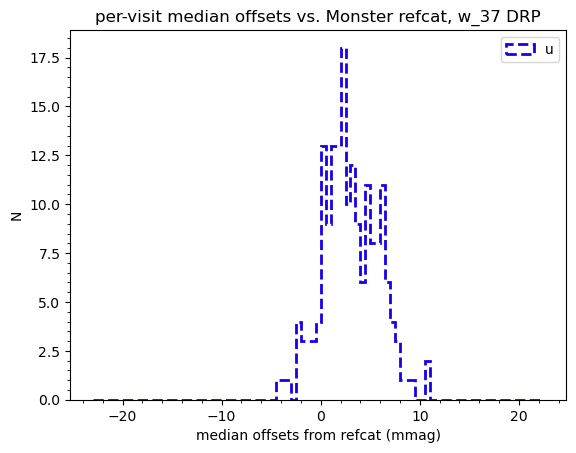
\includegraphics[keepaspectratio]{jira_imgs//zephyr2.png}}\\


}
  {

\begin{tabular}{p{4cm}p{12cm}}
\toprule
Step LVV-E4068-4 & Step Execution Status: \textbf{ Pass } \\ \hline
\end{tabular}
 Description \\
{\footnotesize
Confirm that the PA3u value is less than 20 mmag for the u-band data.

}
\hdashrule[0.5ex]{\textwidth}{1pt}{3mm}
  Test Data \\
 {\footnotesize
None

}
\hdashrule[0.5ex]{\textwidth}{1pt}{3mm}
  Expected Result \\
{\footnotesize

}
\hdashrule[0.5ex]{\textwidth}{1pt}{3mm}
  Actual Result \\
{\footnotesize
We calculated statistics on each of the distributions from the figure
above, and found the following:\\
\strut \\


}
  % end if not not executed - no steps if not executed
\paragraph{ LVV-T1845 - Verify accuracy of photometric transformation to physical scale }\mbox{}\\

Version \textbf{1.0(d)}.
Status \textbf{Approved}.
Open  \href{https://rubinobs.atlassian.net/projects/LVV?selectedItem=com.atlassian.plugins.atlassian-connect-plugin:com.kanoah.test-manager__main-project-page\#\!/v2/testCase/LVV-T1845}{\textit{ LVV-T1845 } }
test case in Jira.

Verify that the DM system provides software to assess whether the
accuracy of the transformation of internal LSST photometry to a physical
scale (e.g. AB magnitudes) is less than \textbf{PA6 = 10
millimagnitudes}.

\textbf{ Preconditions}:\\ None


Execution status: {\bf Pass }\\
Final comment:\\Test performed using DRP processing of LSSTComCam data from Data Preview
1. This was necessary because there are not yet any LSSTCam observations
containing absolute flux standards in all passbands. The notebook where
calculations were performed is attached to this Report\textquotesingle s
git repository as test\_LVV-T1845.ipynb.



% Note Steps "Not Executed" and with No Result are not shown in this report if the flag is passed
Detailed steps results LVV-R293-LVV-E4069-1895464723:\\
  {

\begin{tabular}{p{4cm}p{12cm}}
\toprule
Step LVV-E4069-1 & Step Execution Status: \textbf{ Pass } \\ \hline
\end{tabular}
 Description \\
{\footnotesize
Identify spectrophotometric standard stars that have been observed as
part of a processed dataset.

}
\hdashrule[0.5ex]{\textwidth}{1pt}{3mm}
  Test Data \\
 {\footnotesize
None

}
\hdashrule[0.5ex]{\textwidth}{1pt}{3mm}
  Expected Result \\
{\footnotesize
One or more standards with well-calibrated absolute fluxes to which
measured photometry can be compared.

}
\hdashrule[0.5ex]{\textwidth}{1pt}{3mm}
  Actual Result \\
{\footnotesize
The Calspec standard C26202 was observed with LSSTComCam and was part of
Data Preview 1.


}
  {

\begin{tabular}{p{4cm}p{12cm}}
\toprule
Step LVV-E4069-2 & Step Execution Status: \textbf{ Pass } \\ \hline
\end{tabular}
 Description \\
{\footnotesize
Find all visits in which the standards appear.

}
\hdashrule[0.5ex]{\textwidth}{1pt}{3mm}
  Test Data \\
 {\footnotesize
None

}
\hdashrule[0.5ex]{\textwidth}{1pt}{3mm}
  Expected Result \\
{\footnotesize

}
\hdashrule[0.5ex]{\textwidth}{1pt}{3mm}
  Actual Result \\
{\footnotesize
In the attached notebook, one can see that we identified 710
`visit\_image` datasets containing C26202, of which 668 of the `source`
catalog entries pass the data quality flag cuts.


}
  {

\begin{tabular}{p{4cm}p{12cm}}
\toprule
Step LVV-E4069-3 & Step Execution Status: \textbf{ Pass } \\ \hline
\end{tabular}
 Description \\
{\footnotesize
Calculate synthetic AB magnitudes for the standard stars, using the
standard Rubin bandpasses and published Calspec (or other) SEDs.

}
\hdashrule[0.5ex]{\textwidth}{1pt}{3mm}
  Test Data \\
 {\footnotesize
None

}
\hdashrule[0.5ex]{\textwidth}{1pt}{3mm}
  Expected Result \\
{\footnotesize
Predicted magnitudes in all LSST passbands.

}
\hdashrule[0.5ex]{\textwidth}{1pt}{3mm}
  Actual Result \\
{\footnotesize
The attached notebook demonstrates the use of the system characteristics
and throughputs from `syseng\_throughputs` to integrate the SED of
C26202 and derive magnitudes in LSSTComCam passbands.


}
  {

\begin{tabular}{p{4cm}p{12cm}}
\toprule
Step LVV-E4069-4 & Step Execution Status: \textbf{ Pass } \\ \hline
\end{tabular}
 Description \\
{\footnotesize
Extract `source` table measurements of the standards, and calculate the
median offset between the measured values and the synthetic (predicted)
AB magnitudes. Confirm that the offsets are less than PA6=10 mmag.

}
\hdashrule[0.5ex]{\textwidth}{1pt}{3mm}
  Test Data \\
 {\footnotesize
None

}
\hdashrule[0.5ex]{\textwidth}{1pt}{3mm}
  Expected Result \\
{\footnotesize
Median offsets in all LSST passbands for each standard star.

}
\hdashrule[0.5ex]{\textwidth}{1pt}{3mm}
  Actual Result \\
{\footnotesize
The attached notebook compiles all measurements in each band, then
compares them to synthetic magnitudes from C26202. Comparisons are made
to both an empirical (HST-derived) SED and a model SED from fitting to
the empirical spectrum. The offsets are as follows:\\

\begin{verbatim}
u-band; empirical SED offset: 50.46 mmag; model SED offset: 36.30 mmag
g-band; empirical SED offset: 7.03 mmag; model SED offset: 6.27 mmag
r-band; empirical SED offset: 5.05 mmag; model SED offset: 5.41 mmag
i-band; empirical SED offset: 0.59 mmag; model SED offset: 1.24 mmag
z-band; empirical SED offset: 3.78 mmag; model SED offset: 3.77 mmag
y-band; empirical SED offset: 3.26 mmag; model SED offset: 3.22 mmag
\end{verbatim}

\hfill\break
We see that in all bands except u, the offsets are less than the
required threshold of 10 mmag.\\
\strut \\
We have demonstrated the capability of calculating the accuracy of
transformation to a physical scale (i.e., AB magnitudes) exists.
However, the required accuracy is not met for u-band. Given that the
present test was executed on LSSTComCam data, we will assess the result
as a Pass, but revisit this test when sufficient LSSTCam data are
available.


}
  % end if not not executed - no steps if not executed
  %end of the if with theo test_items in testcycles_map[cyclie.id]



% This appendix is put in as part of the template. You may edit and add to it.
% It is not overwritten by Docsteady.

\newpage
\appendix
\section{Documentation}
The verification process is defined in \citeds{LSE-160}.
The use of Docsteady to format Jira information in various test and planing documents is
described in \citeds{DMTN-140} and practical commands are given in \citeds{DMTN-178}.

\section{Acronyms used in this document}\label{sec:acronyms}
\input{acronyms.tex}

\newpage

% Uncomment this if Docsteady makes you additional appendix
%\input{DMTR-441.appendix.tex}

\end{document}
